\documentclass[]{report}
\usepackage{longtable}
\usepackage{graphicx}
\usepackage{subcaption}
\usepackage{wrapfig}
\usepackage{rotating}
\usepackage[section]{placeins}
\usepackage[margin=1in]{geometry}


% Title Page
\title{Pre-Launch Report}
\author{GWC CanSat}


\begin{document}
\maketitle

\tableofcontents
\listoffigures
\chapter{Introduction}
\section{Team Organization and Roles}

\begin{center}
	\begin{longtable}{rp{13cm}}		
		Team Member&Anna Lee \\
		Role&Teacher \\
		Background&Teacher of physics at George Watson's College \\
		Responsibilities&In charge of competing administrative paperwork for the team, and organizing travel\\
		\hline
		Team Member&Kaveh Pezeshki \\
		Role&Team Leader, Electronics Design and Assembly, Mechanical Design, Software Development \\
		Background&Key interests in physics, computer science, electrical and mechanical engineering, maths \\
		Responsibilities&Founded the team, communicated with sponsors and school administration and registered the team for the UK and EU competitions. Continued as a sponsor liaison and contact point for the team, as well as handling administrative tasks. Designed the overall system architecture, selected components, designed electrical layouts, and built the prototype cansat electronics board by hand. Assisted in component choice for the second revision, drew rough schematics, and prepared the completed PCBs. Brainstormed design ideas, drew CAD models of the CanSat design, and communicated with sponsors to build the prototype internal frame. Chose internal frame materials, and communicated with sponsors to create a complete physical 3D printed model of the internal frame. Used python to design and write the prototype CanSat and base station software, including packetization, independent data logging, multithreading, sensor control, and an interactive GUI.
		\\
		Time Committed&Approximately 500 hours out of school\\
		\hline
		Team Member&Calder Maclean \\
		Role&Software Development \\
		Background&Key interests in software and computer science \\
		Responsibilities&Programmed the CanSat module and onboard modules to read ambient humidity and temperature, GPS positioning, thermal imaging, etc. The CanSat stores raw data on board and transmits live data to the base station via a radio module\\
		Time Committed&Approximately 150 hours out of school\\
		\hline
		Team Member&Charles Cameron \\
		Role&Electronics design, mechanical assembly and outreach \\
		Background&Interested in physics, computer science, electrical and mechanical engineering, maths \\
		Responsibilities&CAD designed the PCB layout of electronic sub-systems using EAGLE for the second revision, as well as producing a bill of materials for the PCB assembly house. Liaison with sponsors and PCB manufacturers for assembly/implementation of a custom printed PCB. In charge of ordering team supplies and CanSat equipment, as well as keeping track of team expenses. Designed the GWC CanSat website and contributed to general outreach. Collaborated in constructing the CanSat outer shell.
		Prepared the prototype and final CanSat internal frames for implementation into the assembly \\
		Time Committed&Approximately 500 hours out of school\\
		\hline
		Team Member&Jack Hargreaves \\
		Role&Software Development \\
		Background&Key interests in software and computer science \\
		Responsibilities&Developed base station software to interpret incoming data from the CanSat which is then displayed in multiple graphs in real-time, as well as being stored onboard. In addition, the status of all sensors is displayed in a visual representation of the CanSat.\\
		Time Committed&Approximately 200 hours out of school\\
		\hline
		Team Member&Pedro Guimaraes \\
		Role&Mechanical Design \\
		Background&Key interests in computer science, maths, and chemistry \\
		Responsibilities&Designed and constructed prototypes for the CanSat outer shell. Brainstormed and constructed prototypes for test fixture release mechanisms for the CanSat.\\
		Time Committed&Approximately 100 hours out of school\\
		\hline
		Team Member&Morven Pennie \\
		Role&Outreach Representative, Mechanical Design, Graphical Designer \\
		Background&Key interests in computer science, graphic design, mechanical engineering and art \\
		Responsibilities&Brainstormed and designed team graphics for the team website, social media and public events, such as the Edinburgh Mini Maker Faire. Designed and coordinated team apparel and CanSat external graphics. Collaborated in constructing the CanSat outer shell. Lead social media representative for the team, including taking/gathering promotional photos. Animated the CanSat logo for promotional videos in addition to editing the team videos.\\
		Time Committed&Approximately 400 hours out of school\\
	\end{longtable}
\end{center}

\section{Mission Objectives}
\subsection{Secondary Mission}
GWC CanSat's secondary mission covers two main targets:

Initially, the CanSat is intended to monitor several variables in the general atmosphere, this covers ambient temperature, humidity, and barometric pressure. This aims to support existing hypotheses about trends associated with these variables.

We also aim to create heat maps of the surface below the CanSat. This requires the capability to accurately and precisely monitor the orientation and position of the CanSat, in addition to using precise thermal imaging.
\subsection{Launch Objectives}
In order for a successful flight of our CanSat, we require all the onboard sensors to perform accurately, precisely and reliably. This involves factors such as adequate vibration control, secure electrical connections to the modules, sufficient cooling throughout the CanSat and internal levels around the electronics.

To produce an accurate and precise heat map, it is necessary for us to accurately track CanSat position: this is done through the use of pressure-based altitude calculations, IMU integration, and a GPS.

In addition, we require a stable radio connection between our base station and our CanSat. To achieve this, we have purchased a Yagi-Uda antenna and tested (to the best of our ability) the transmit/receive range between the base station and radio module.
\subsection{Expected Results}
We expect to establish clear trends in the ambient temperature, humidity, and pressure. These trends should hopefully support existing hypotheses about the relationships between altitude and the previously stated variables.

We also expect to construct a heat map of the surface below the CanSat, which will allow us to determine any major thermal activity happening in the target area.
\subsection{Experimental and Data Logging Aims}
Our CanSat is equipped with a range of sensor modules, capable of recording data on the ambient temperature, humidity, barometric pressure, altitude, GPS longitude, GPS latitude and 3-axis rotation, as well as being equipped with a thermal sensor for surface thermal imaging.

This will allow us to determine several general atmospheric trends which we intend to compare with existing hypotheses. We expect no discrepancies, so these experiments will contribute as supporting evidence.

We will also use the thermal imaging feed, GPS positioning, and rotation data to construct a precise heat map of the surroundings, this will allow us to investigate any significant and/or unexpected thermal activity in the area around the CanSat launch zone. This can be applied for environmental and emission surveys and allow us to further investigate outdoor heat gains, heat vents, and cool zones.

\chapter{CanSat Description}
\section{Mission Overview}
In general terms, our team has divided our CanSat goals into two categories. First of all, we've designed our CanSat to monitor general atmospheric trends, via temperature, barometric pressure, and humidity sensors.

Secondly, our CanSat is also capable of constructing a heat map of the below surface. In order to accomplish this goal, our CanSat needs to be able to precisely track its orientation and position, as well as measure temperature of the ground surface below the CanSat.

We've included a high-precision IMU (Inertial Measurement Unit) incorporating a three-axis gyroscope, three-axis magnetometer, and three-axis compass to provide accurate orientation data via a digital prediction filter, as well as a GPS to compensate for drift in the calculated CanSat position. We've also included a low-resolution thermal camera facing from the bottom of our CanSat. Through these sensors, the CanSat is able to map incoming thermal camera data to the region of the ground surface from which it originates, allowing construction of a large-scale temperature map as the CanSat drifts over the ground surface.

A Linux single board computer and Arduino Pro Mini allow for redundant data logging and provide enough speed for all necessary calculations to be done on-CanSat, at 10 Hz for environmental sensors and 100-1000Hz for positional tracking sensors.
Data transmission to the base station is accomplished through an XBEE 868LP and GSM radio. The XBEE 868LP serves as our primary method of communication, dynamically updating the base station data store with an update rate depending on packet loss: typically between 2-5Hz.

If communication is lost with the base station due to hardware, software, or packet loss issues, the CanSat will shift to an emergency location tracking mode, reporting hardware or sensor failures as well as GPS position via texts to a team member's cell phone.

A rough visualization of our CanSat electronics system is shown in figure \ref{bdiagram}.

\begin{figure}[h]
	\hfill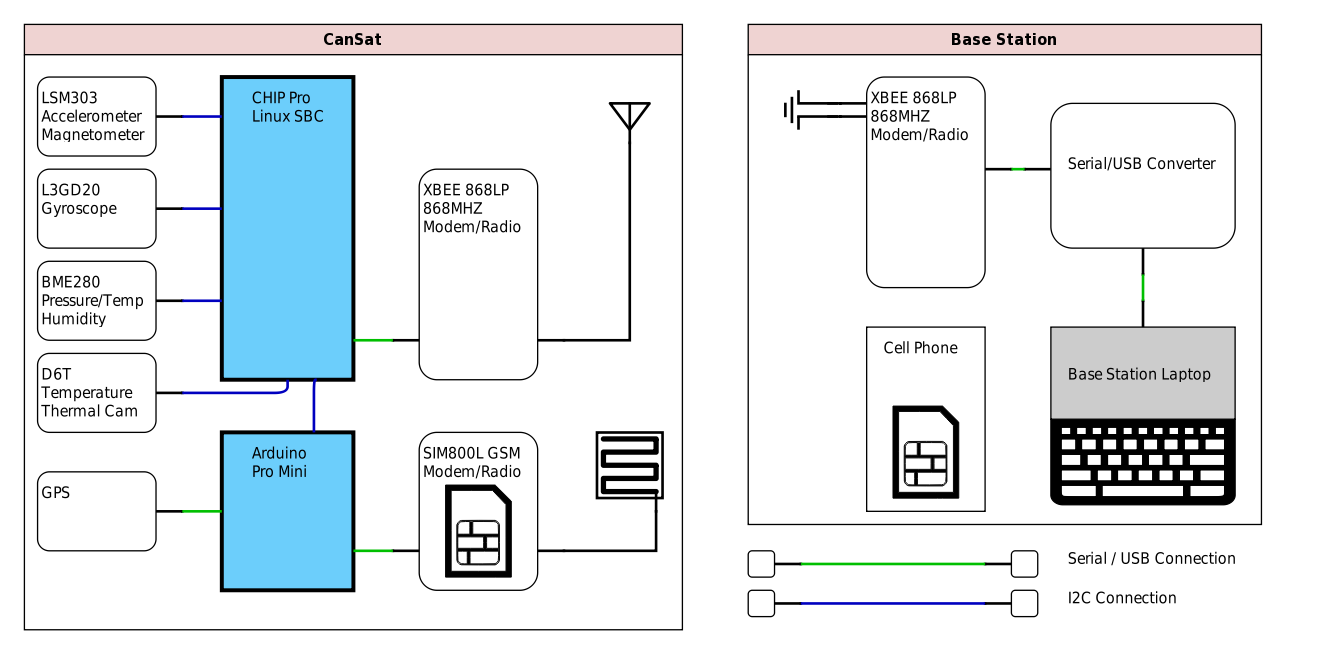
\includegraphics[scale=0.4]{Block_Diagram.png}\hspace*{\fill}
	\caption{CanSat block diagram}
	\label{bdiagram}
\end{figure}


It is also necessary for our CanSat mechanical design to create an environment in which our sensors can operate at peak accuracy. Our CanSat requirements included a durable and shock-resistant design and an unguided descent at 10.5ms-1. We accomplished this via a steel-nylon internal frame, a shock absorbing fiberglass outer shell, and a ripstop nylon parachute.
\section{Mechanical and Structural Design}
\subsection{Overview}
Our team has made use of a variety of materials and assembly techniques in our CanSat structure to optimize CanSat durability, modularity, and weight. In accomplishing this goal, we split CanSat mechanical design into three discrete sections: internal frame, outer shell, and electronics. Our current CanSat design is available in browser on SketchFab \footnote{https://sketchfab.com/cansatgwc}. We've also published the current mechanical design to a GitHub repository \footnote{https://github.com/Arcturus314/cansat2017\_design}.

The development of our final CanSat design has been a long process. To further clarify our design decisions this report will also describe the prototyping process.

To provide context to each section of our CanSat design, CAD-rendered and real-life images of the assembled final and prototype CanSats are shown in figures \ref{oldcansat} and \ref{newcansat} (real life photos do not include the outer shell).

\begin{figure}
	\centering
	\begin{subfigure}{.5\textwidth}
		\centering
		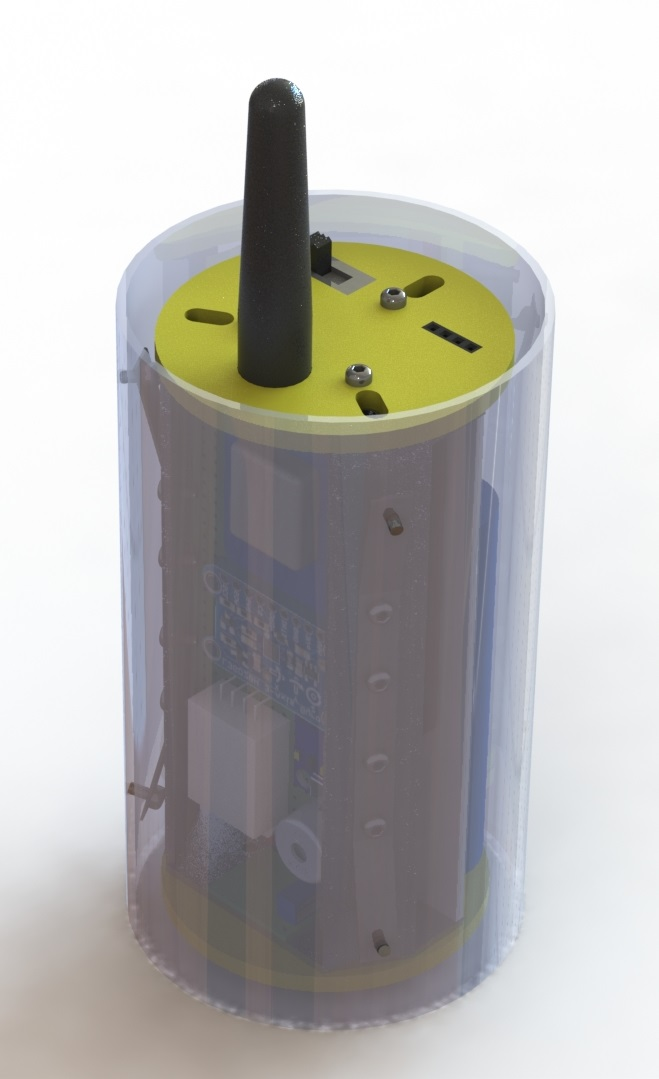
\includegraphics[width=.8\linewidth]{Old_CanSat_render.jpg}
	\end{subfigure}%
	\begin{subfigure}{.5\textwidth}
		\centering
		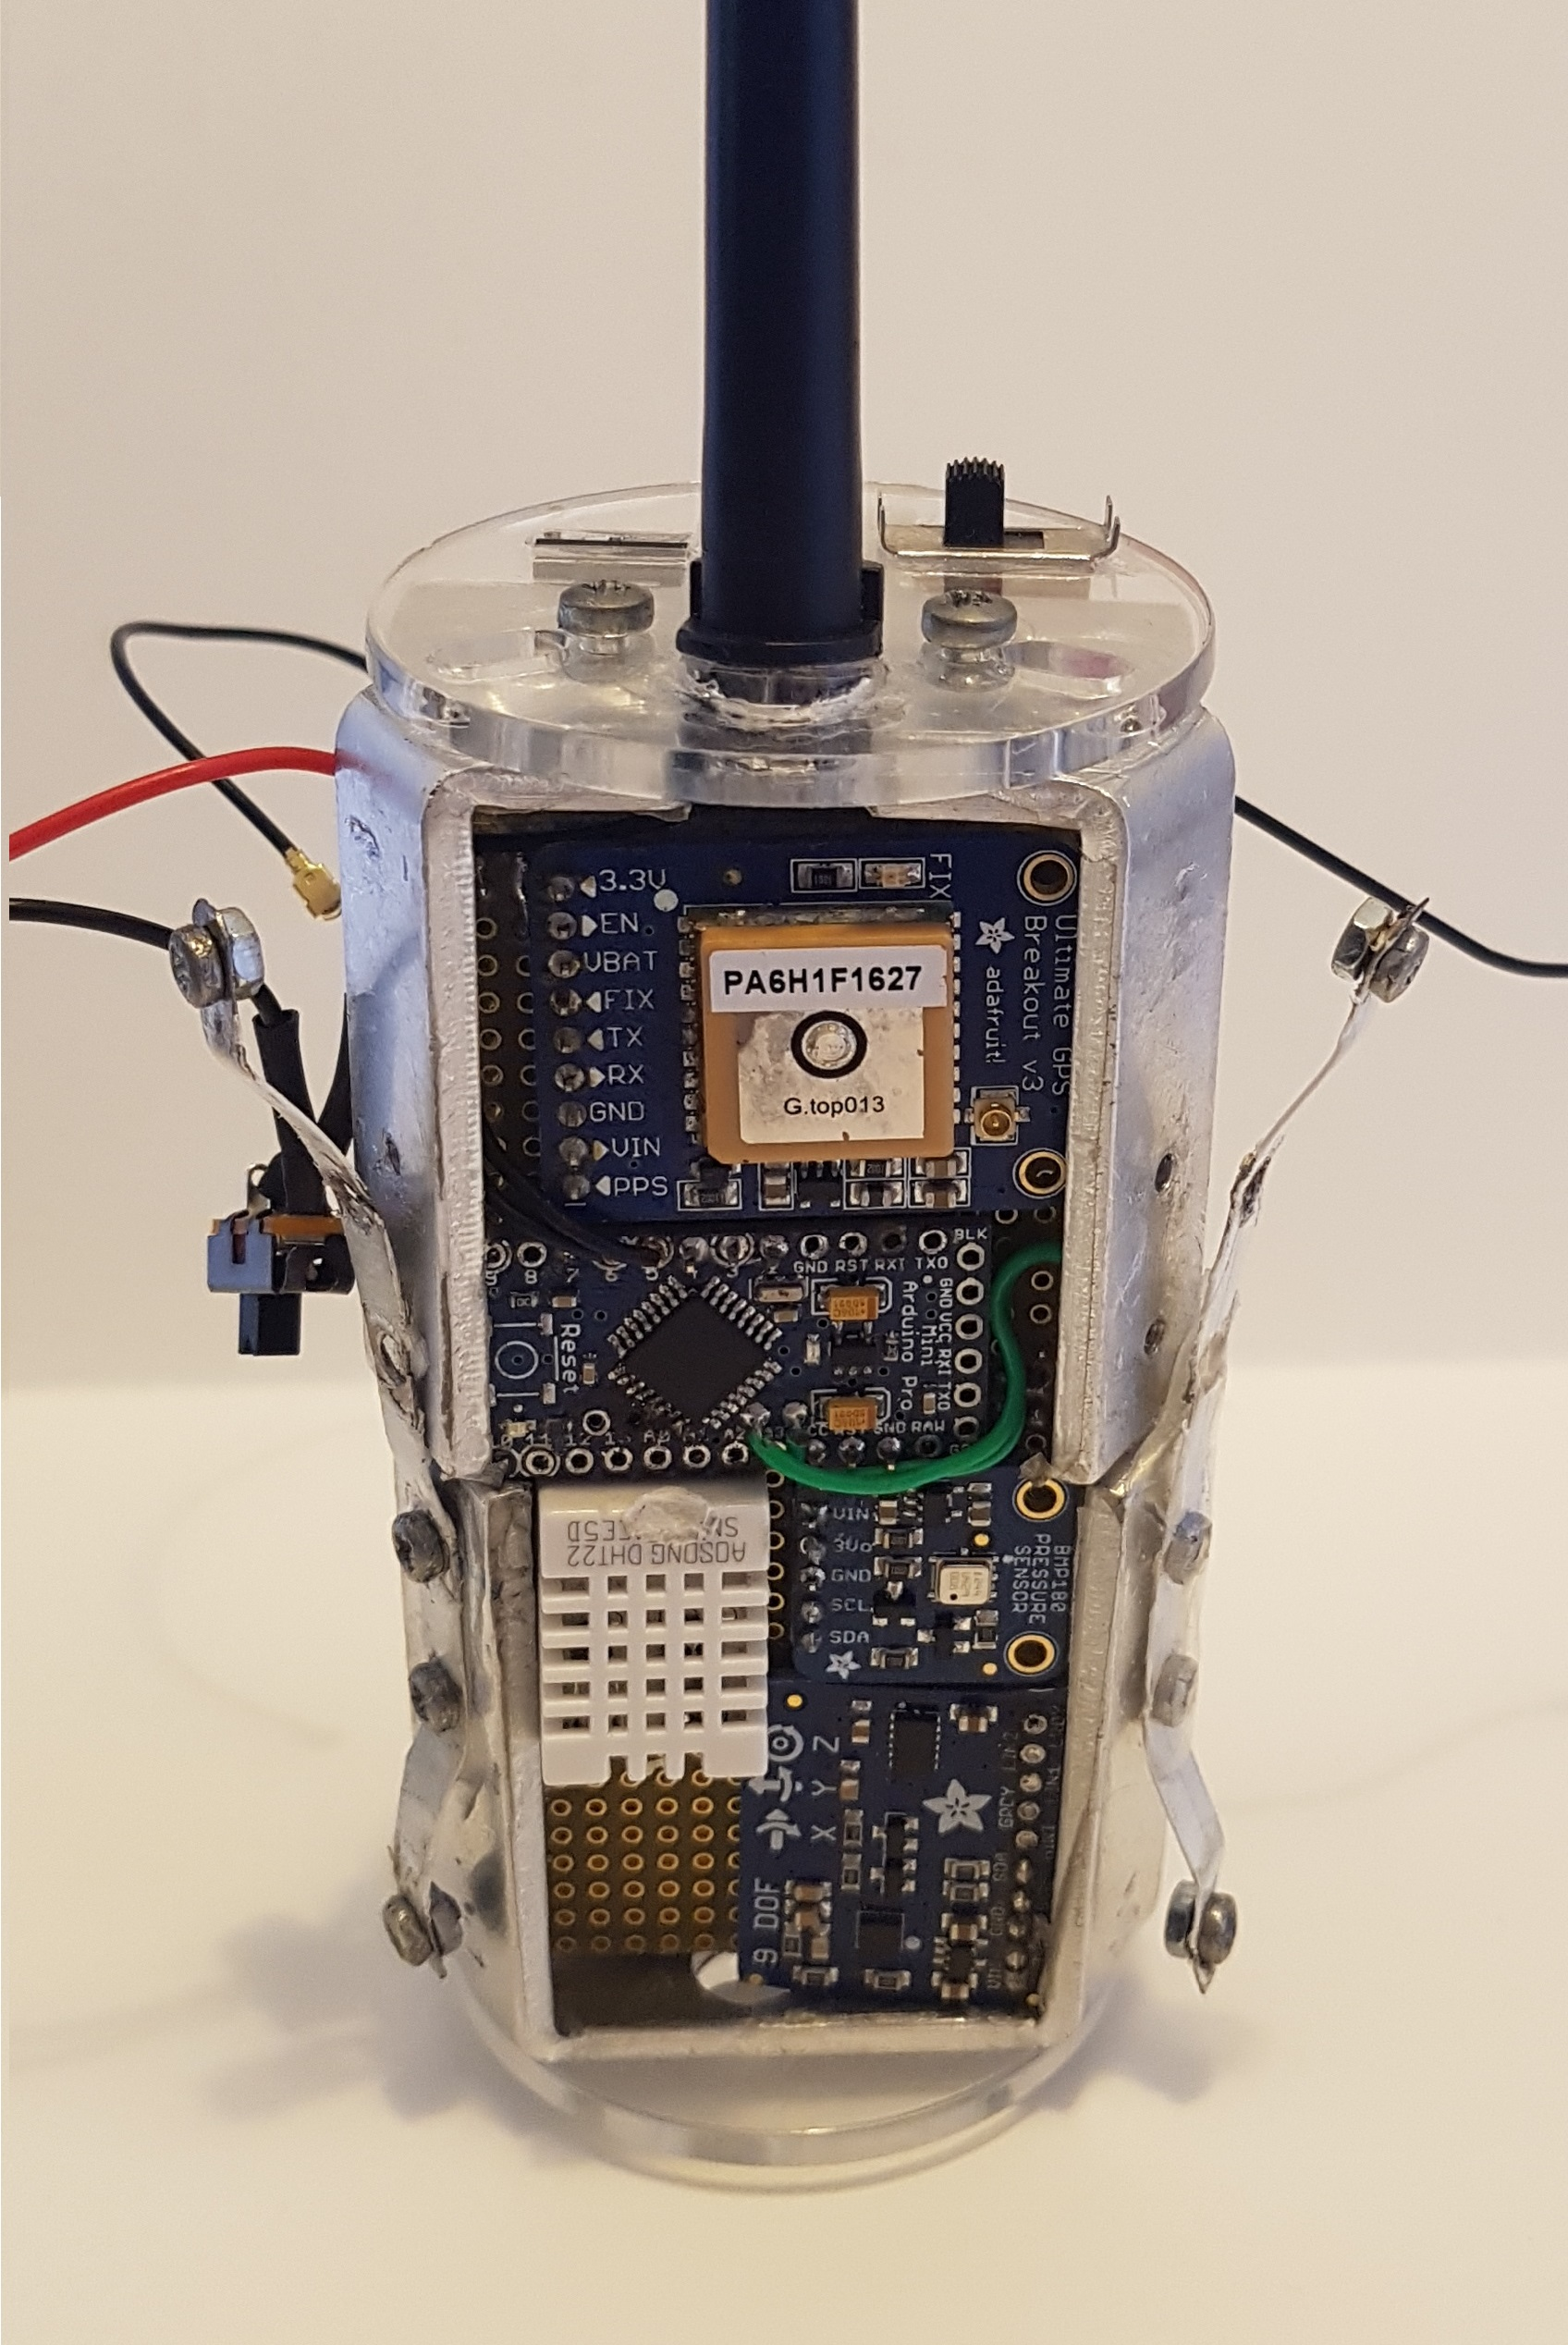
\includegraphics[width=0.8\linewidth, angle=0]{old_cansat.jpg}
	\end{subfigure}
	\caption{Prototype CanSat design}
	\label{oldcansat}
\end{figure}

\begin{figure}
	\centering
	\begin{subfigure}{.5\textwidth}
		\centering
		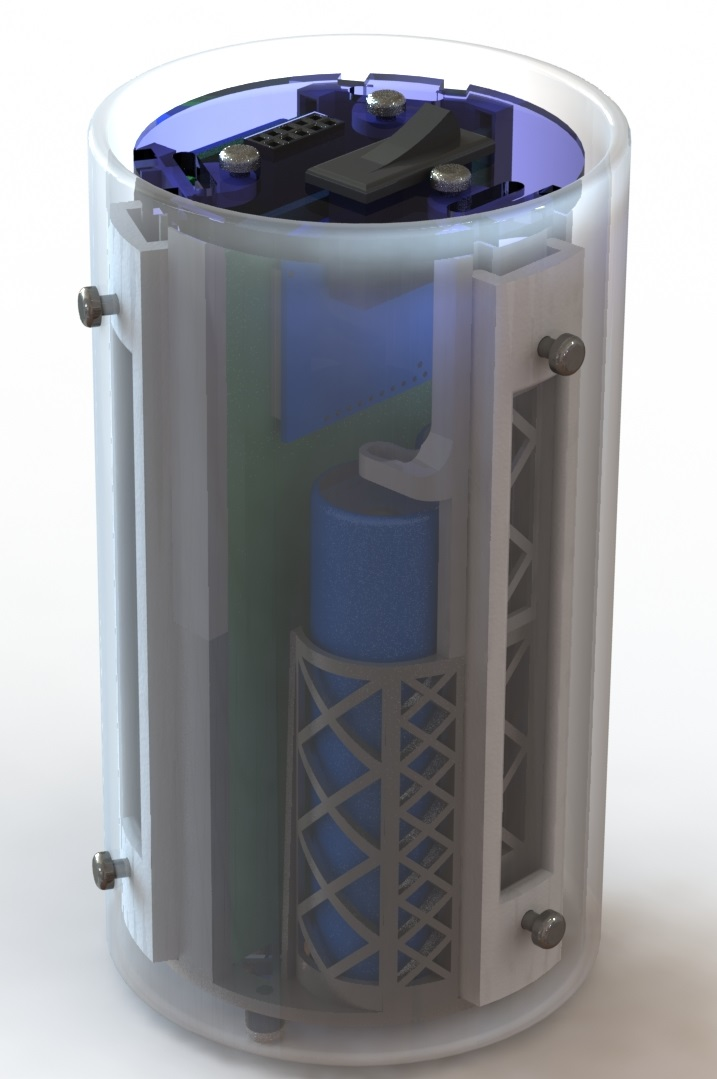
\includegraphics[width=.8\linewidth]{CanSat_render.jpg}
	\end{subfigure}%
	\begin{subfigure}{.5\textwidth}
		\centering
		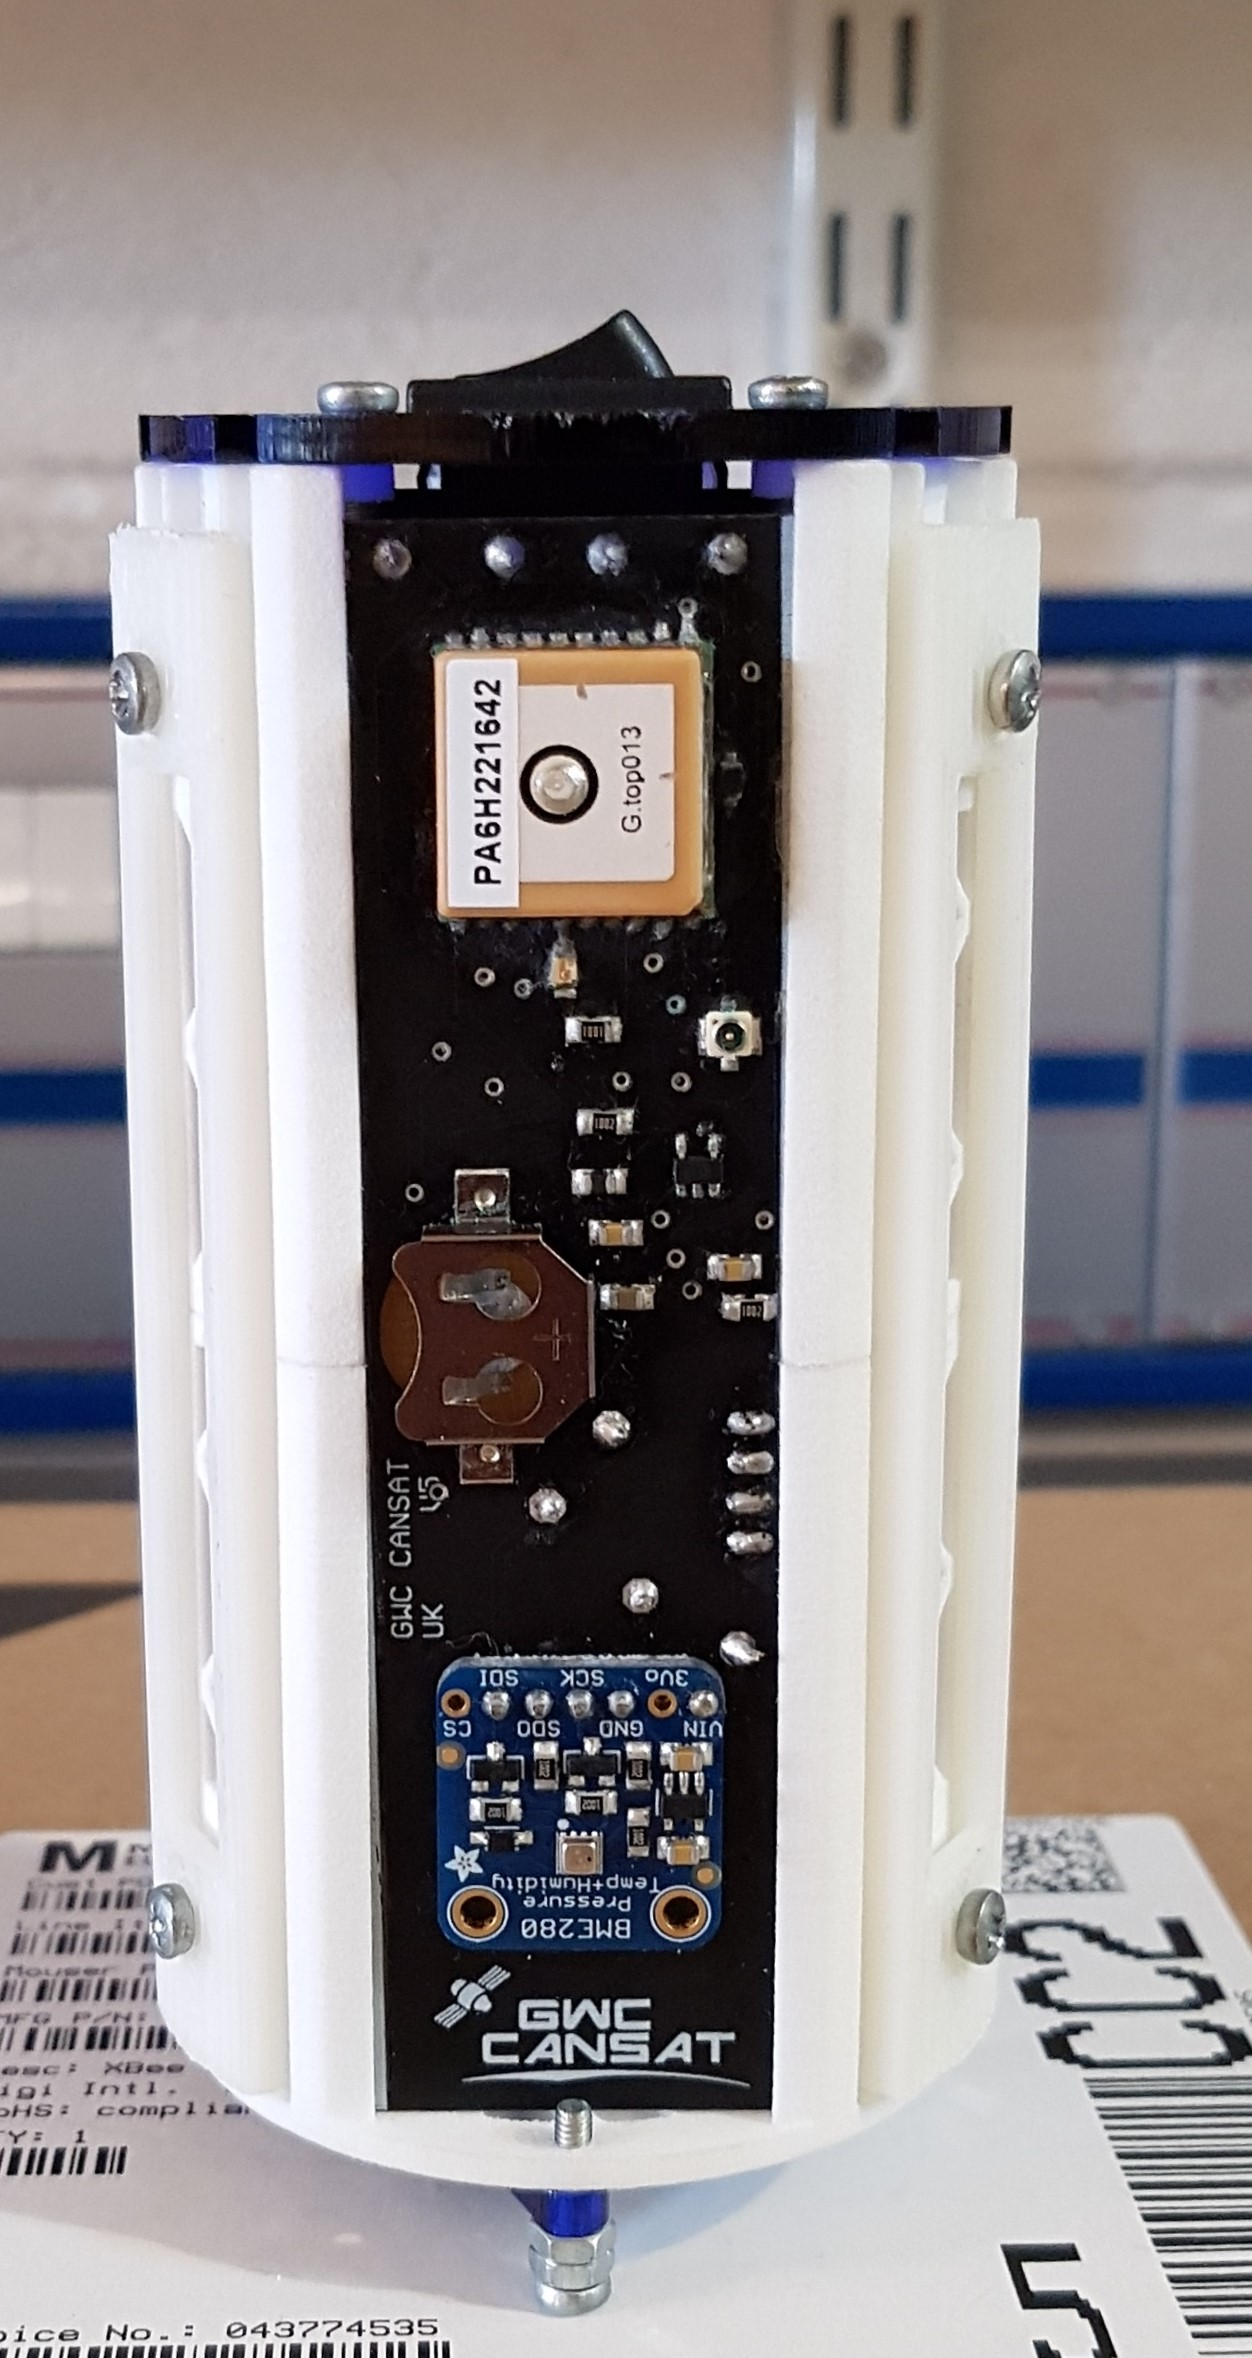
\includegraphics[width=0.6\linewidth]{new_cansat.jpg}
	\end{subfigure}
	\caption{Final CanSat design}
	\label{newcansat}
\end{figure}


\subsection{Internal Frame}
In order to maximize durability the team decided to split the electronics housing into a tough internal frame and relatively flexible outer shell, attached via a simple mounting mechanism. The goal of this design was for the outer shell to absorb the large forces due to ground collision, while the internal frame provides a structural rigidity and another layer of protection for the sensitive electronics
\subsubsection{Prototype Design}
In the development of our internal frame, the team experimented with a variety of materials. As our school stocked 3mm acrylic sheets, we first tested a bent acrylic frame. However, we found that the bend point was lacking the necessary strength for our CanSat, easily shattering on impact. The team then decided to replicate the original design with a bent aluminum frame, seen in figure \ref{intframeold}. 

%\begin{wrapfigure}{r}{0.5\textwidth}
%	\begin{center}
%		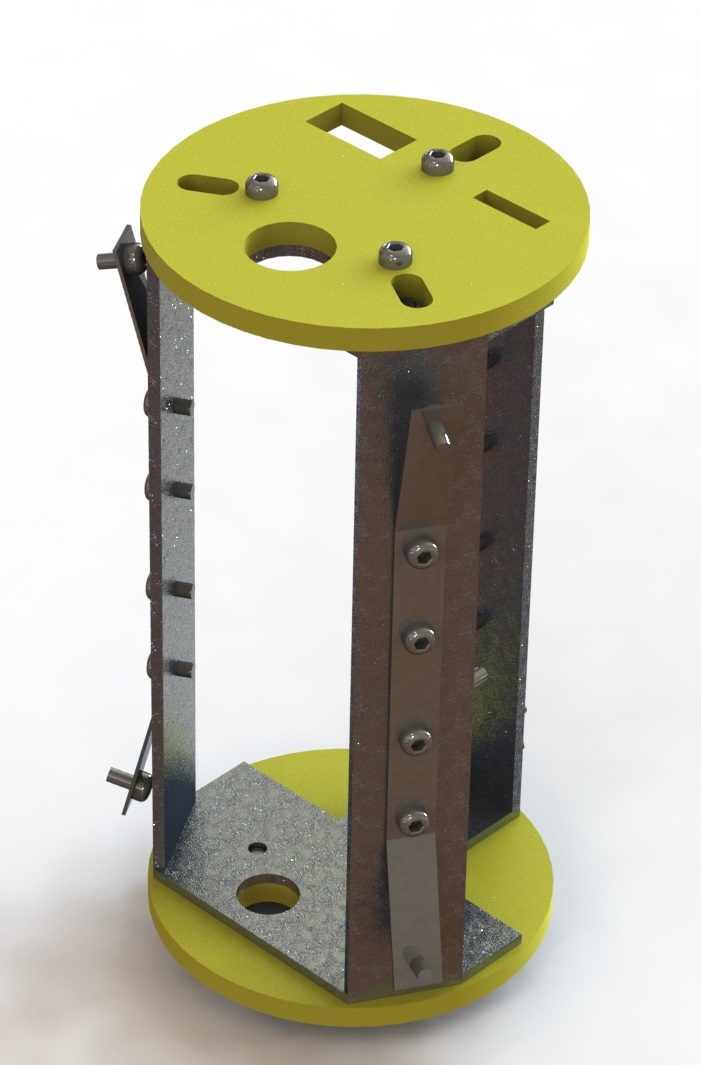
\includegraphics[scale=0.4]{old_int_frame.jpg}
%	\end{center}
%	\caption{Prototype CanSat internal frame}
%	\label{intframeold}
%\end{wrapfigure}

\begin{figure}[h]
	\hfill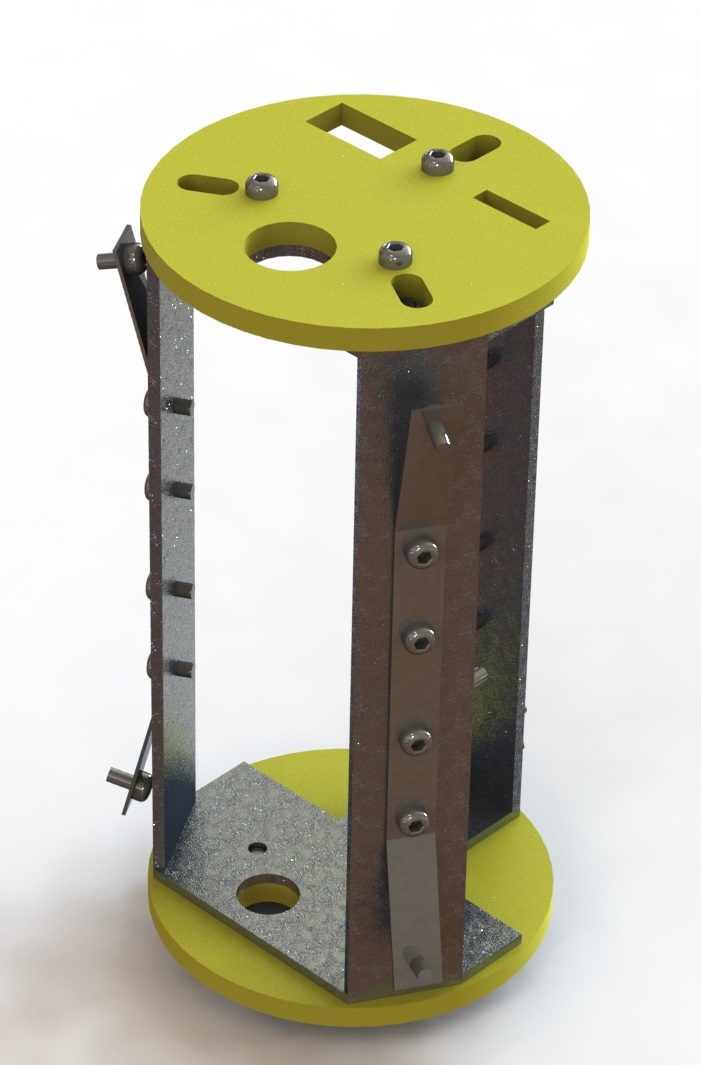
\includegraphics[scale=0.4]{old_int_frame.jpg}\hspace*{\fill}
	\caption{Prototype CanSat internal frame}
	\label{intframeold}
\end{figure}

The aluminum frame provided the required rigidity, strength, and toughness for our prototype design. While the internal frame was still relatively basic, lacking specific PCB and sensor mount points, it fulfilled our design requirements.

As the team had easy access to a laser cutter via our school, we decided to laser cut top and bottom CanSat plates to provide easy mounting points for antennae, switches, and headers.

The development of the CanSat internal frame can be seen via the bottom frames of our prototype CanSat revisions, shown in figure \ref{ointframedev}.


\begin{figure}[h]
	\hfill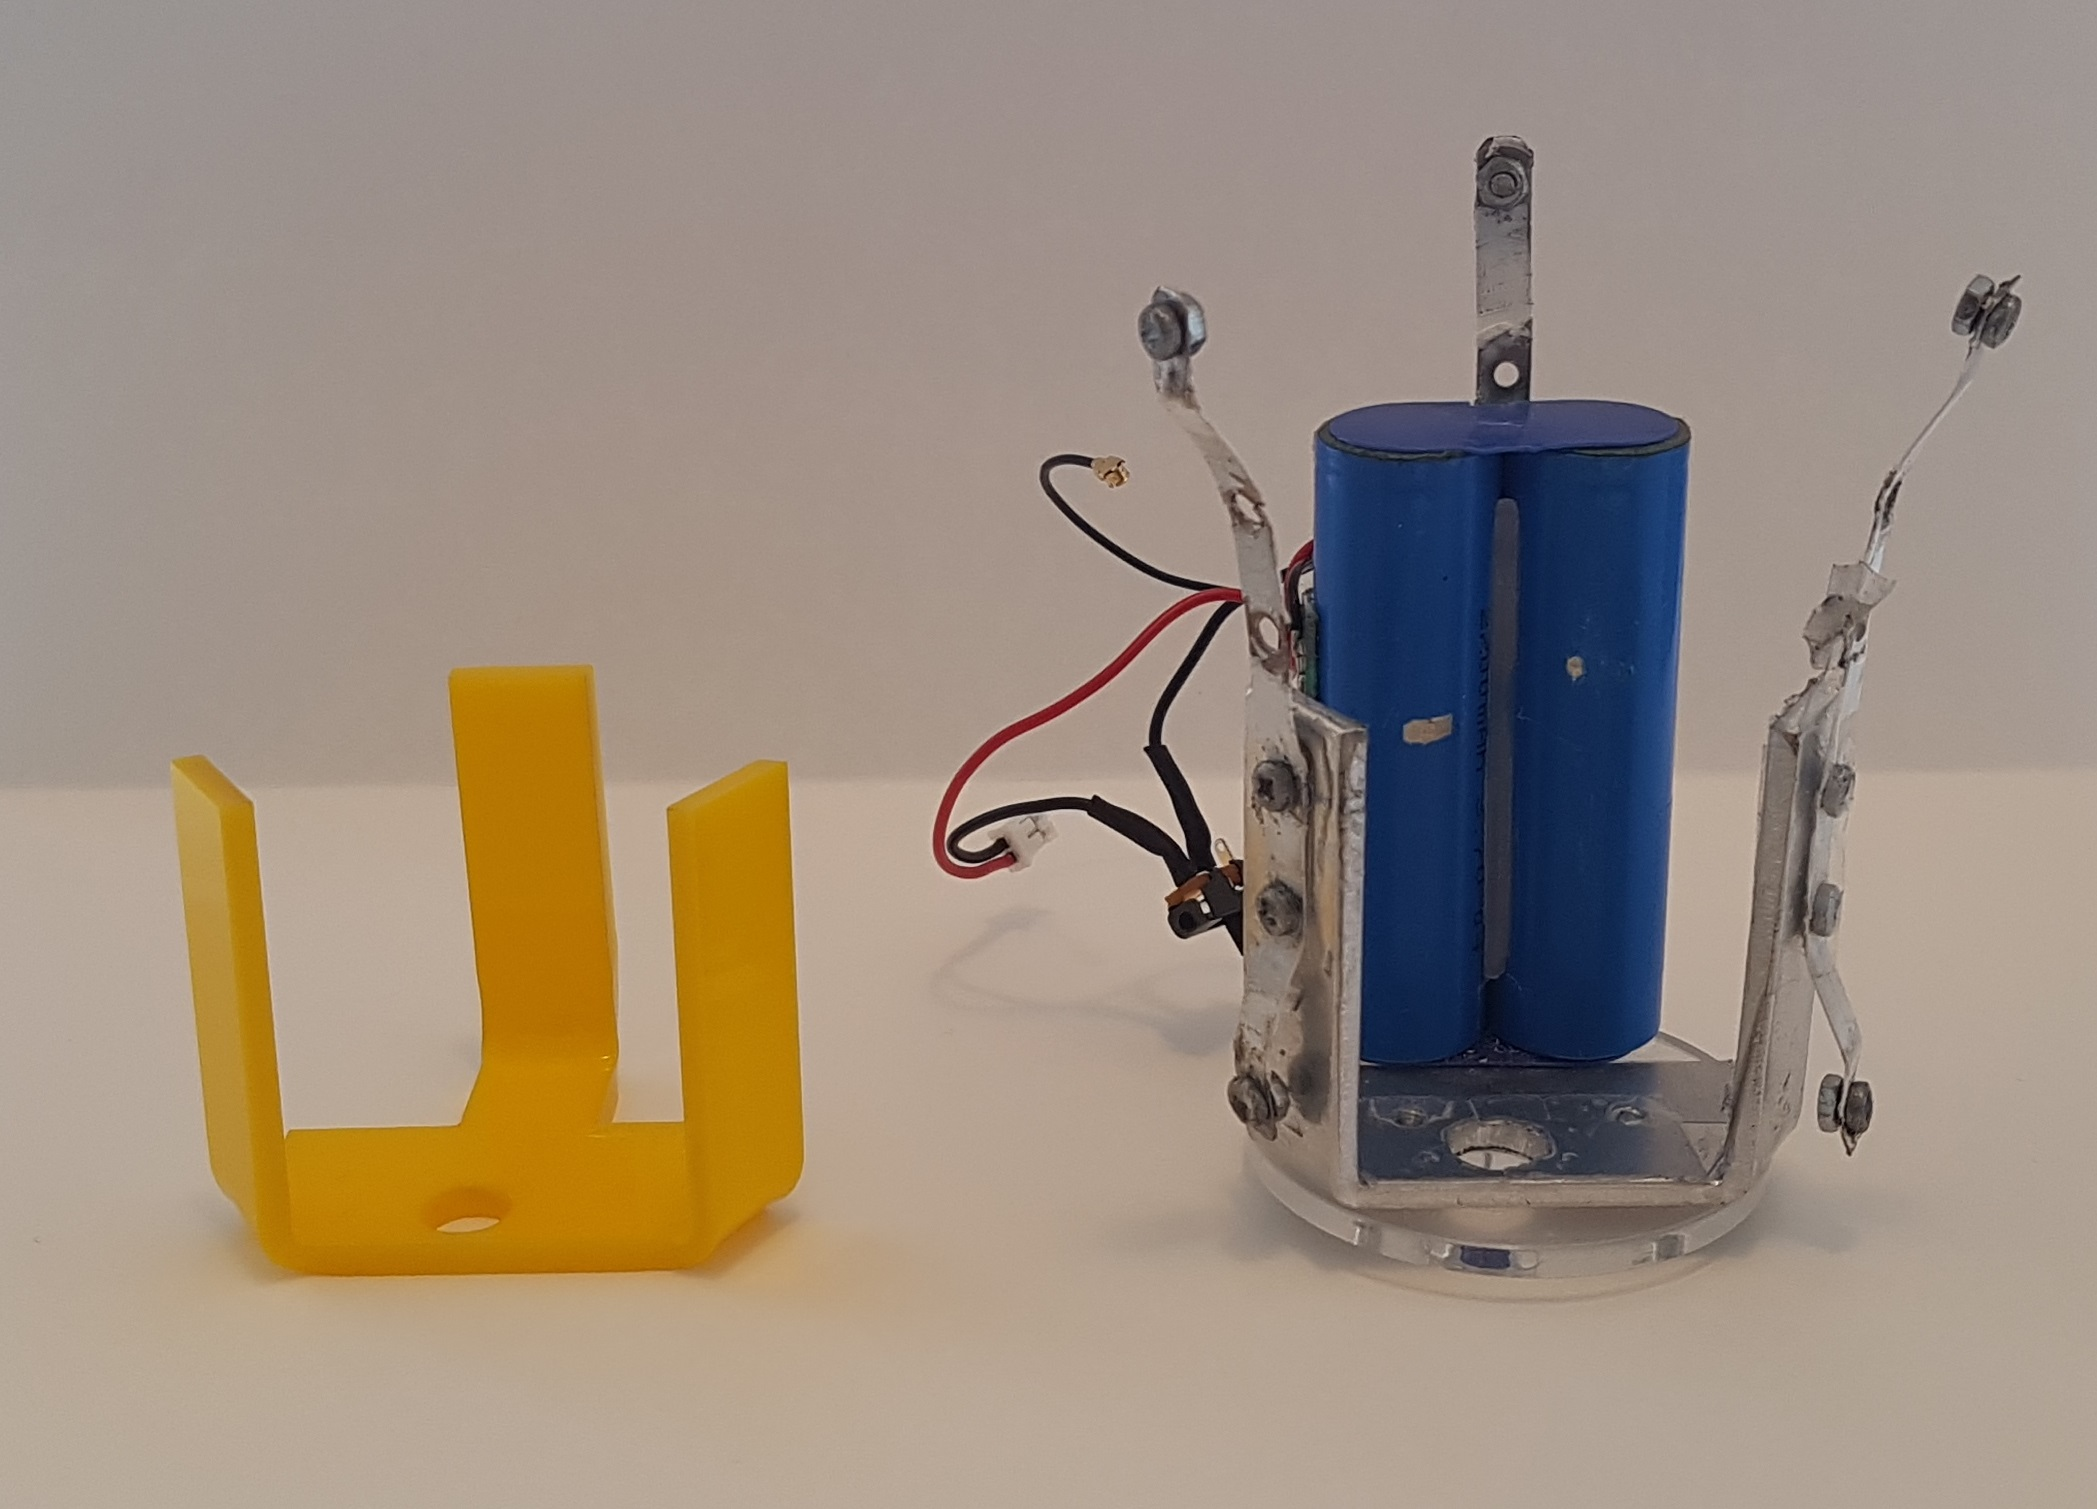
\includegraphics[scale=0.15]{old_frame.jpg}\hspace*{\fill}
	\caption{Prototype CanSat internal frame development}
	\label{ointframedev}
\end{figure}

\subsubsection{Final Design}
In the team's second design revision, we aimed to use additive manufacturing to allow for a more complex internal frame, maximizing strength, minimizing weight, and allowing for sensor, PCB, and battery mounting points directly on the internal frame, as illustrated in figure \ref{newframerender}.

%\begin{wrapfigure}{L}{0.5\textwidth}
%	\begin{center}
%		\includegraphics[scale=0.4]{cansat_internal_frame_render.jpg}
%	\end{center}
%	\caption{Final CanSat internal frame render}
%	\label{newframerender}
%\end{wrapfigure}

\begin{figure}[h]
	\hfill\includegraphics[scale=0.4]{cansat_internal_frame_render.jpg}\hspace*{\fill}
	\caption{Final CanSat internal frame render}
	\label{newframerender}
\end{figure}

We again elected to split the CanSat frame into top and bottom components. The top frame was composed of three discrete vertical support bars, providing slider trenches and screw holes for mounting the outer shell, slots for mounting PCBs, as well as battery-holding prongs and parachute/top plate mounting points. These support bars were attached via a laser-cut top plate, again providing switch and header mounting points, as well as holes to allow for parachute mounts- this is shown in figure \ref{topframerender}.

%\begin{wrapfigure}{R}{0.5\textwidth}
%	\begin{center}
%		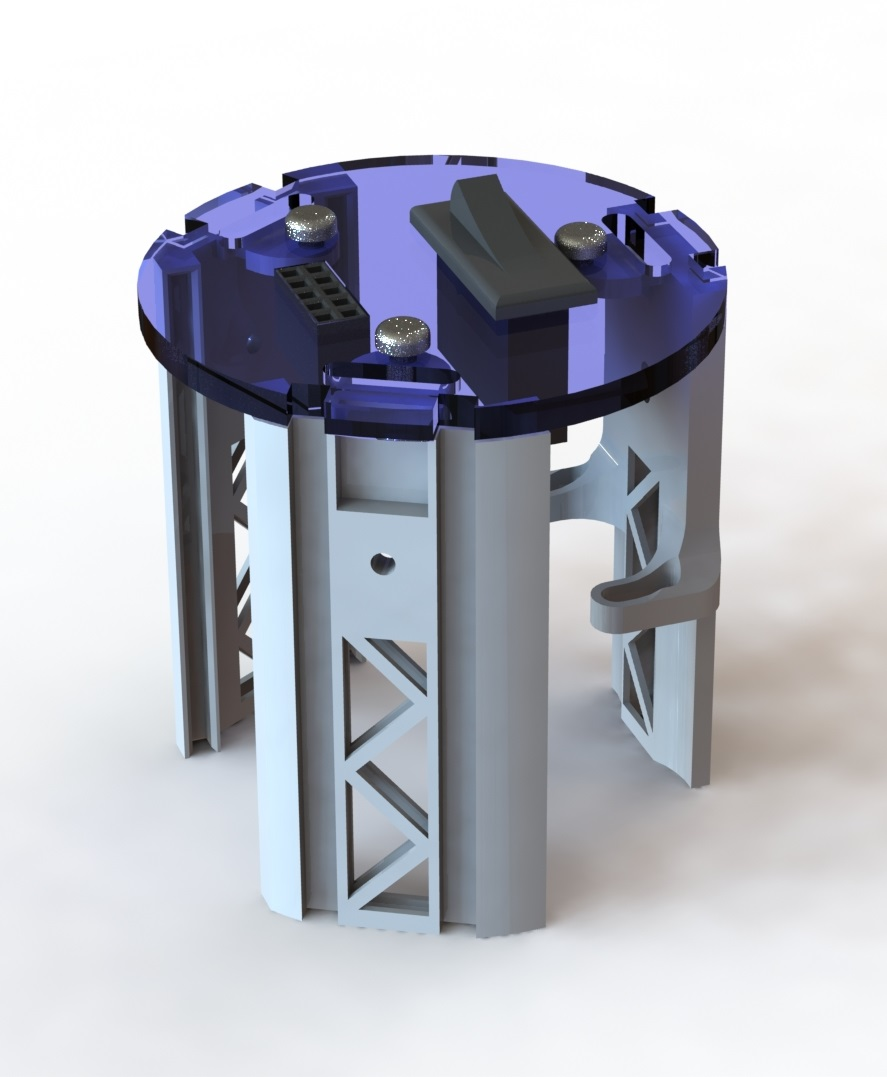
\includegraphics[scale=0.4]{Top_frame_render.jpg}
%	\end{center}
%	\caption{Final CanSat top frame render}
%	\label{topframerender}
%\end{wrapfigure}

\begin{figure}[h]
	\hfill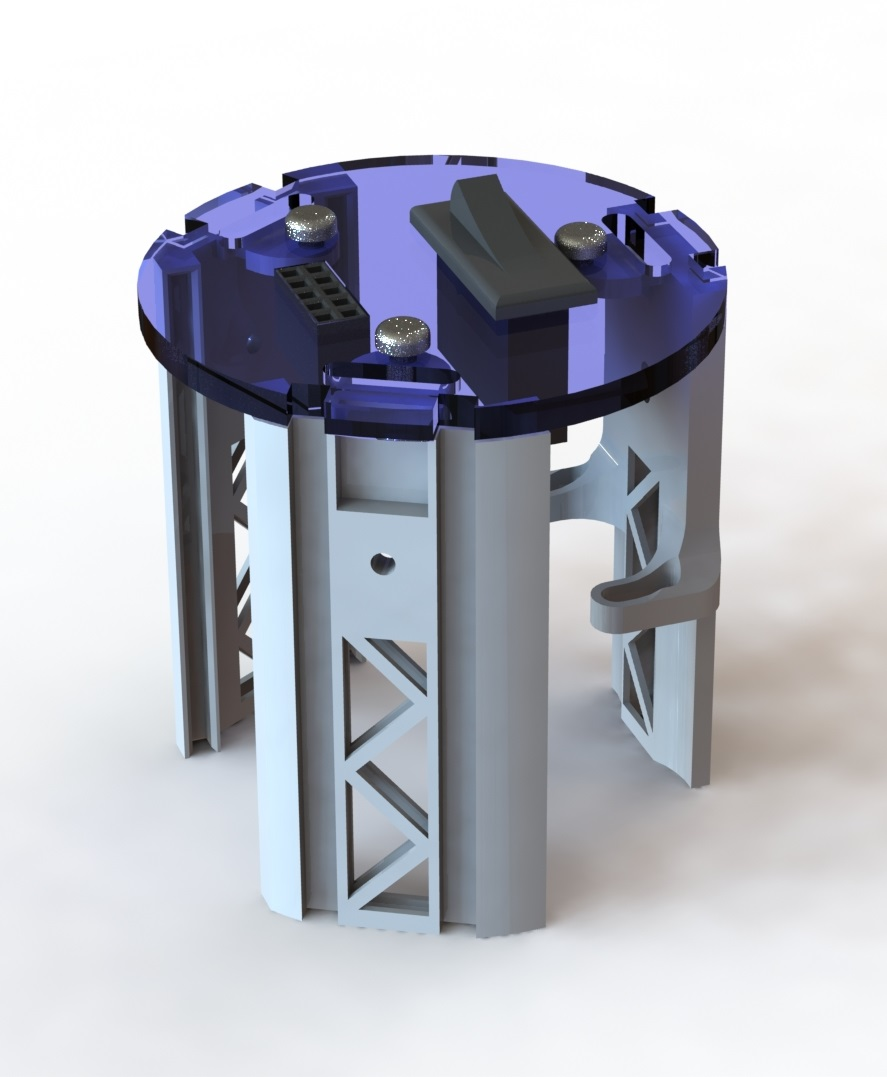
\includegraphics[scale=0.4]{Top_frame_render.jpg}\hspace*{\fill}
	\caption{Final CanSat top frame render}
	\label{topframerender}
\end{figure}

The bottom frame was more complex. The basic frame was designed as a single piece of material, again with outer shell, PCB, and battery mount and hold points. Additionally, the bottom frame includes a mounting plate for an Omron D6T thermal camera, as well as screw holes to allow for add-on modules to be attached to the CanSat. Currently, these screw holes are occupied by a piece of laser-cut plastic providing a protective bezel for the thermal camera, seen in figure \ref{bottomframerender}.

%\begin{wrapfigure}{L}{0.5\textwidth}
%	\begin{center}
%		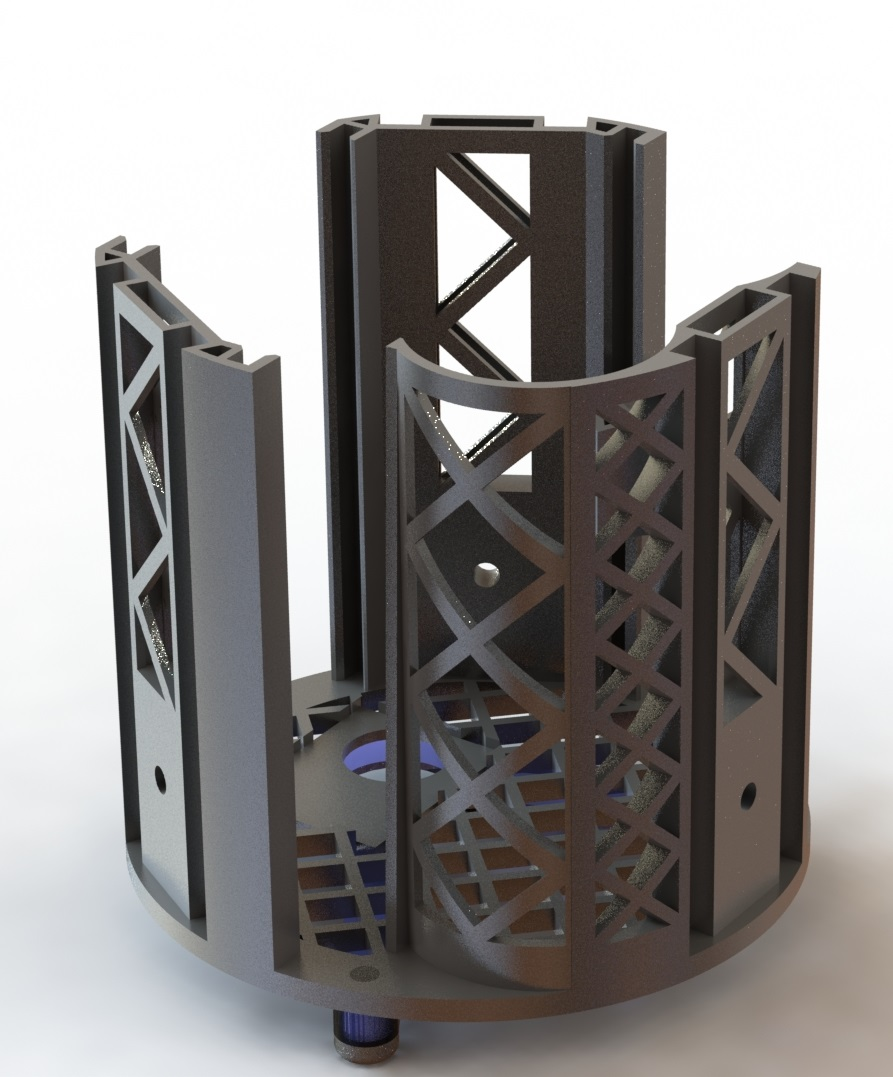
\includegraphics[scale=0.4]{Bottom_frame_render.jpg}
%	\end{center}
%	\caption{Final CanSat bottom frame render}
%	\label{bottomframerender}
%\end{wrapfigure}

\begin{figure}[h]
	\hfill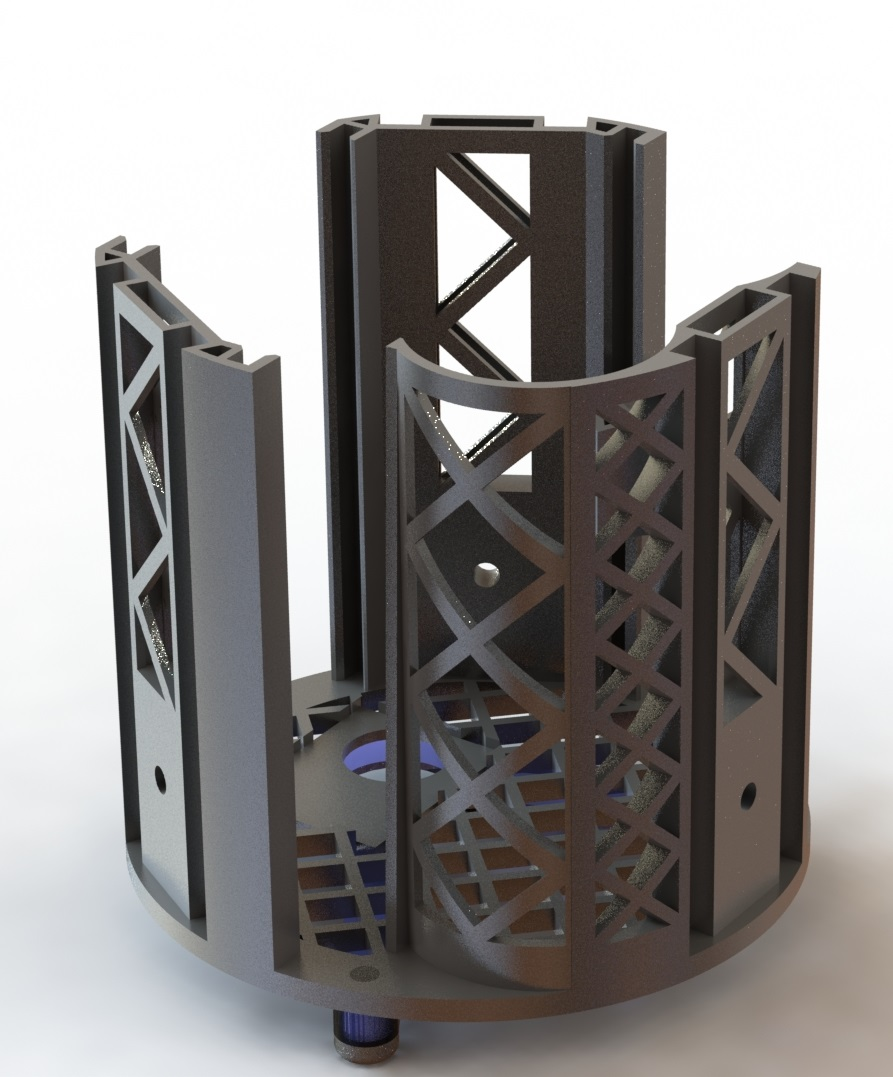
\includegraphics[scale=0.4]{Bottom_frame_render.jpg}\hspace*{\fill}
	\caption{Final CanSat bottom frame render}
	\label{bottomframerender}
\end{figure}

The internal frame was initially designed to be printed from PLA in a consumer 3D printer. However, we found that this did not provide the desired tolerances. This is clearly seen in the image in figure \ref{plaframe}.

\begin{figure}[h]
	\hfill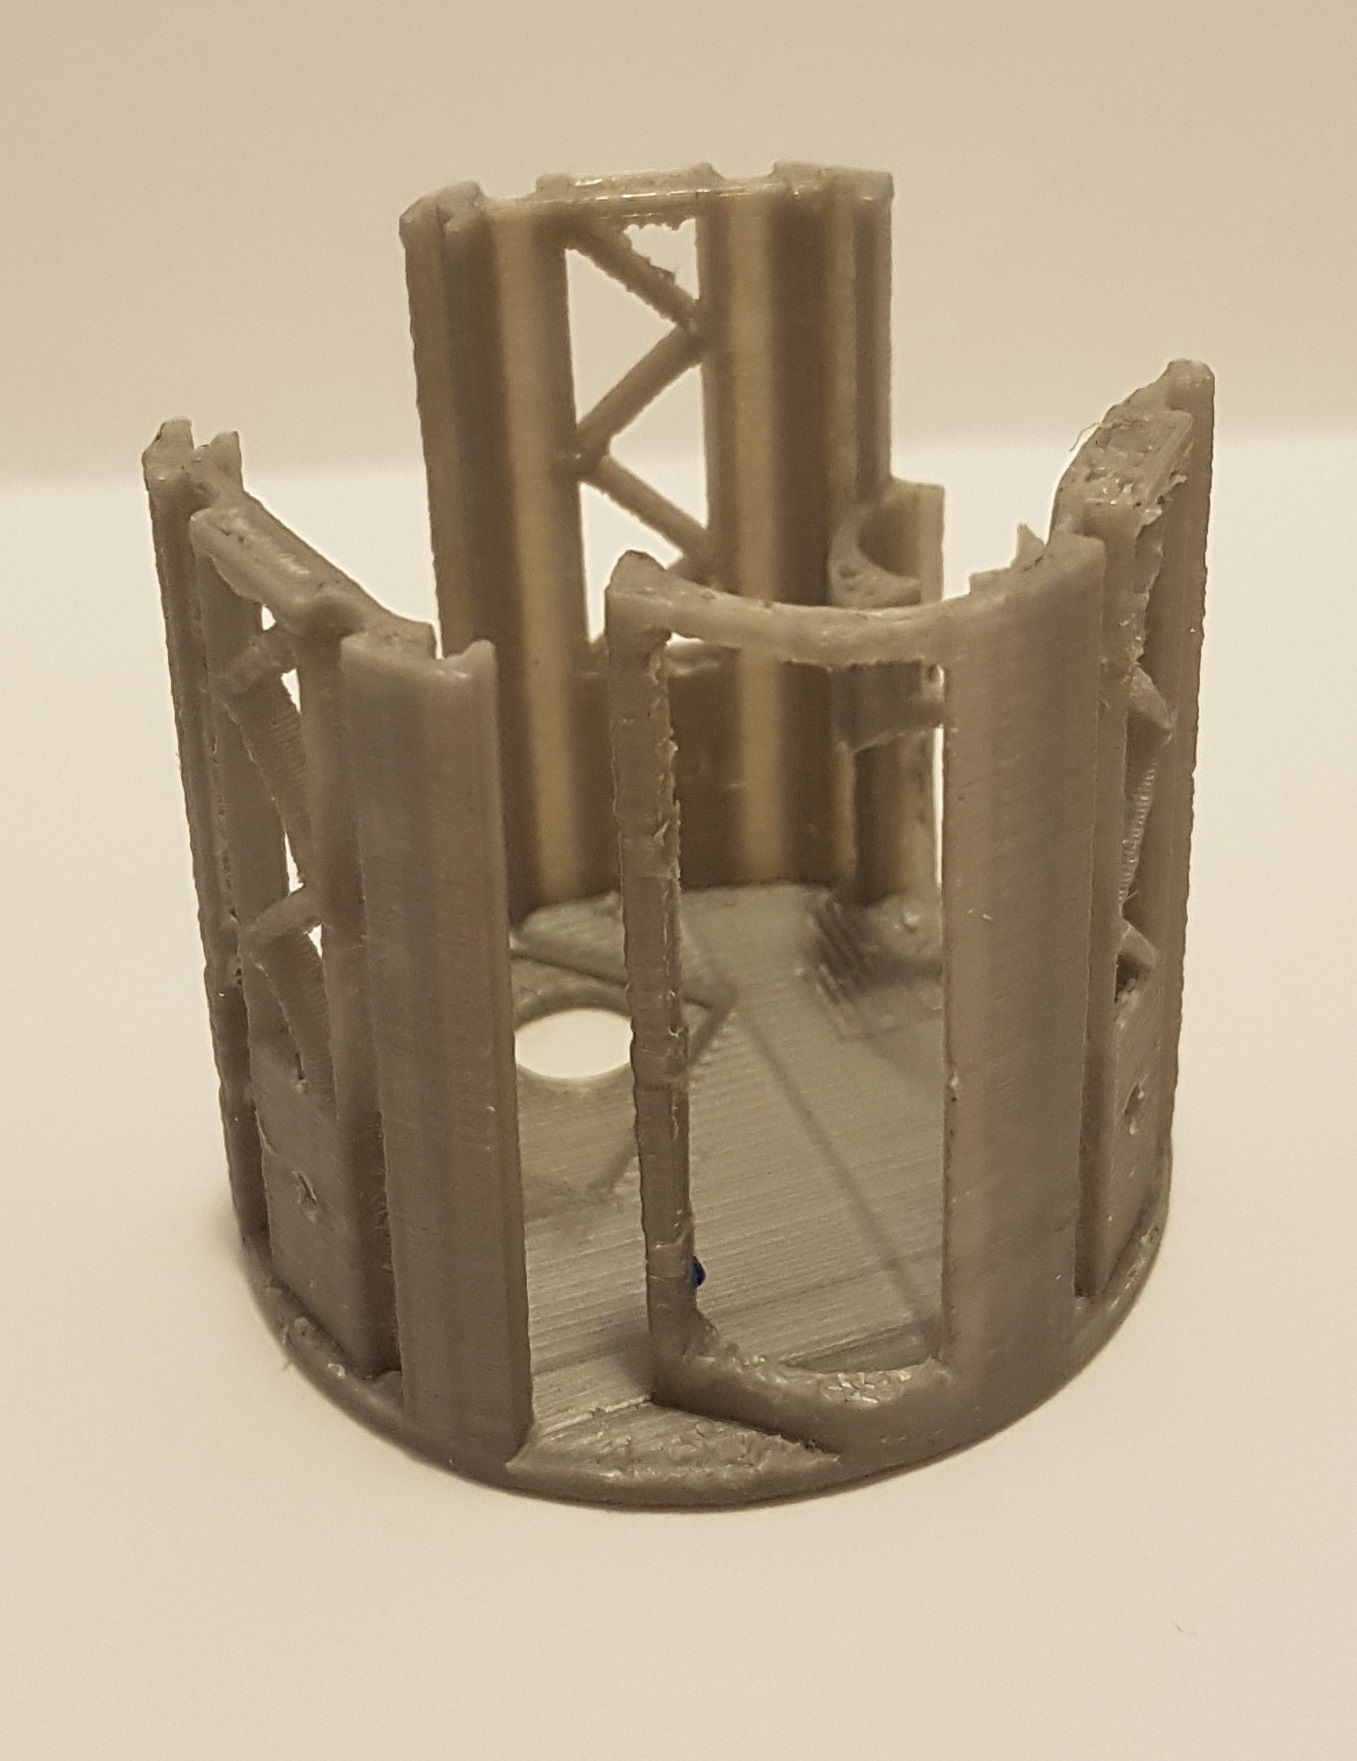
\includegraphics[scale=0.15]{pla_frame.jpg}\hspace*{\fill}
	\caption{A 3D printed PLA CanSat bottom frame}
	\label{plaframe}
\end{figure}


Croft additive manufacturing offered to sponsor the team with an SLS (selective laser sintering) internal frame built from stainless steel, seen in figure \ref{steelframe}.

\begin{figure}[h]
	\hfill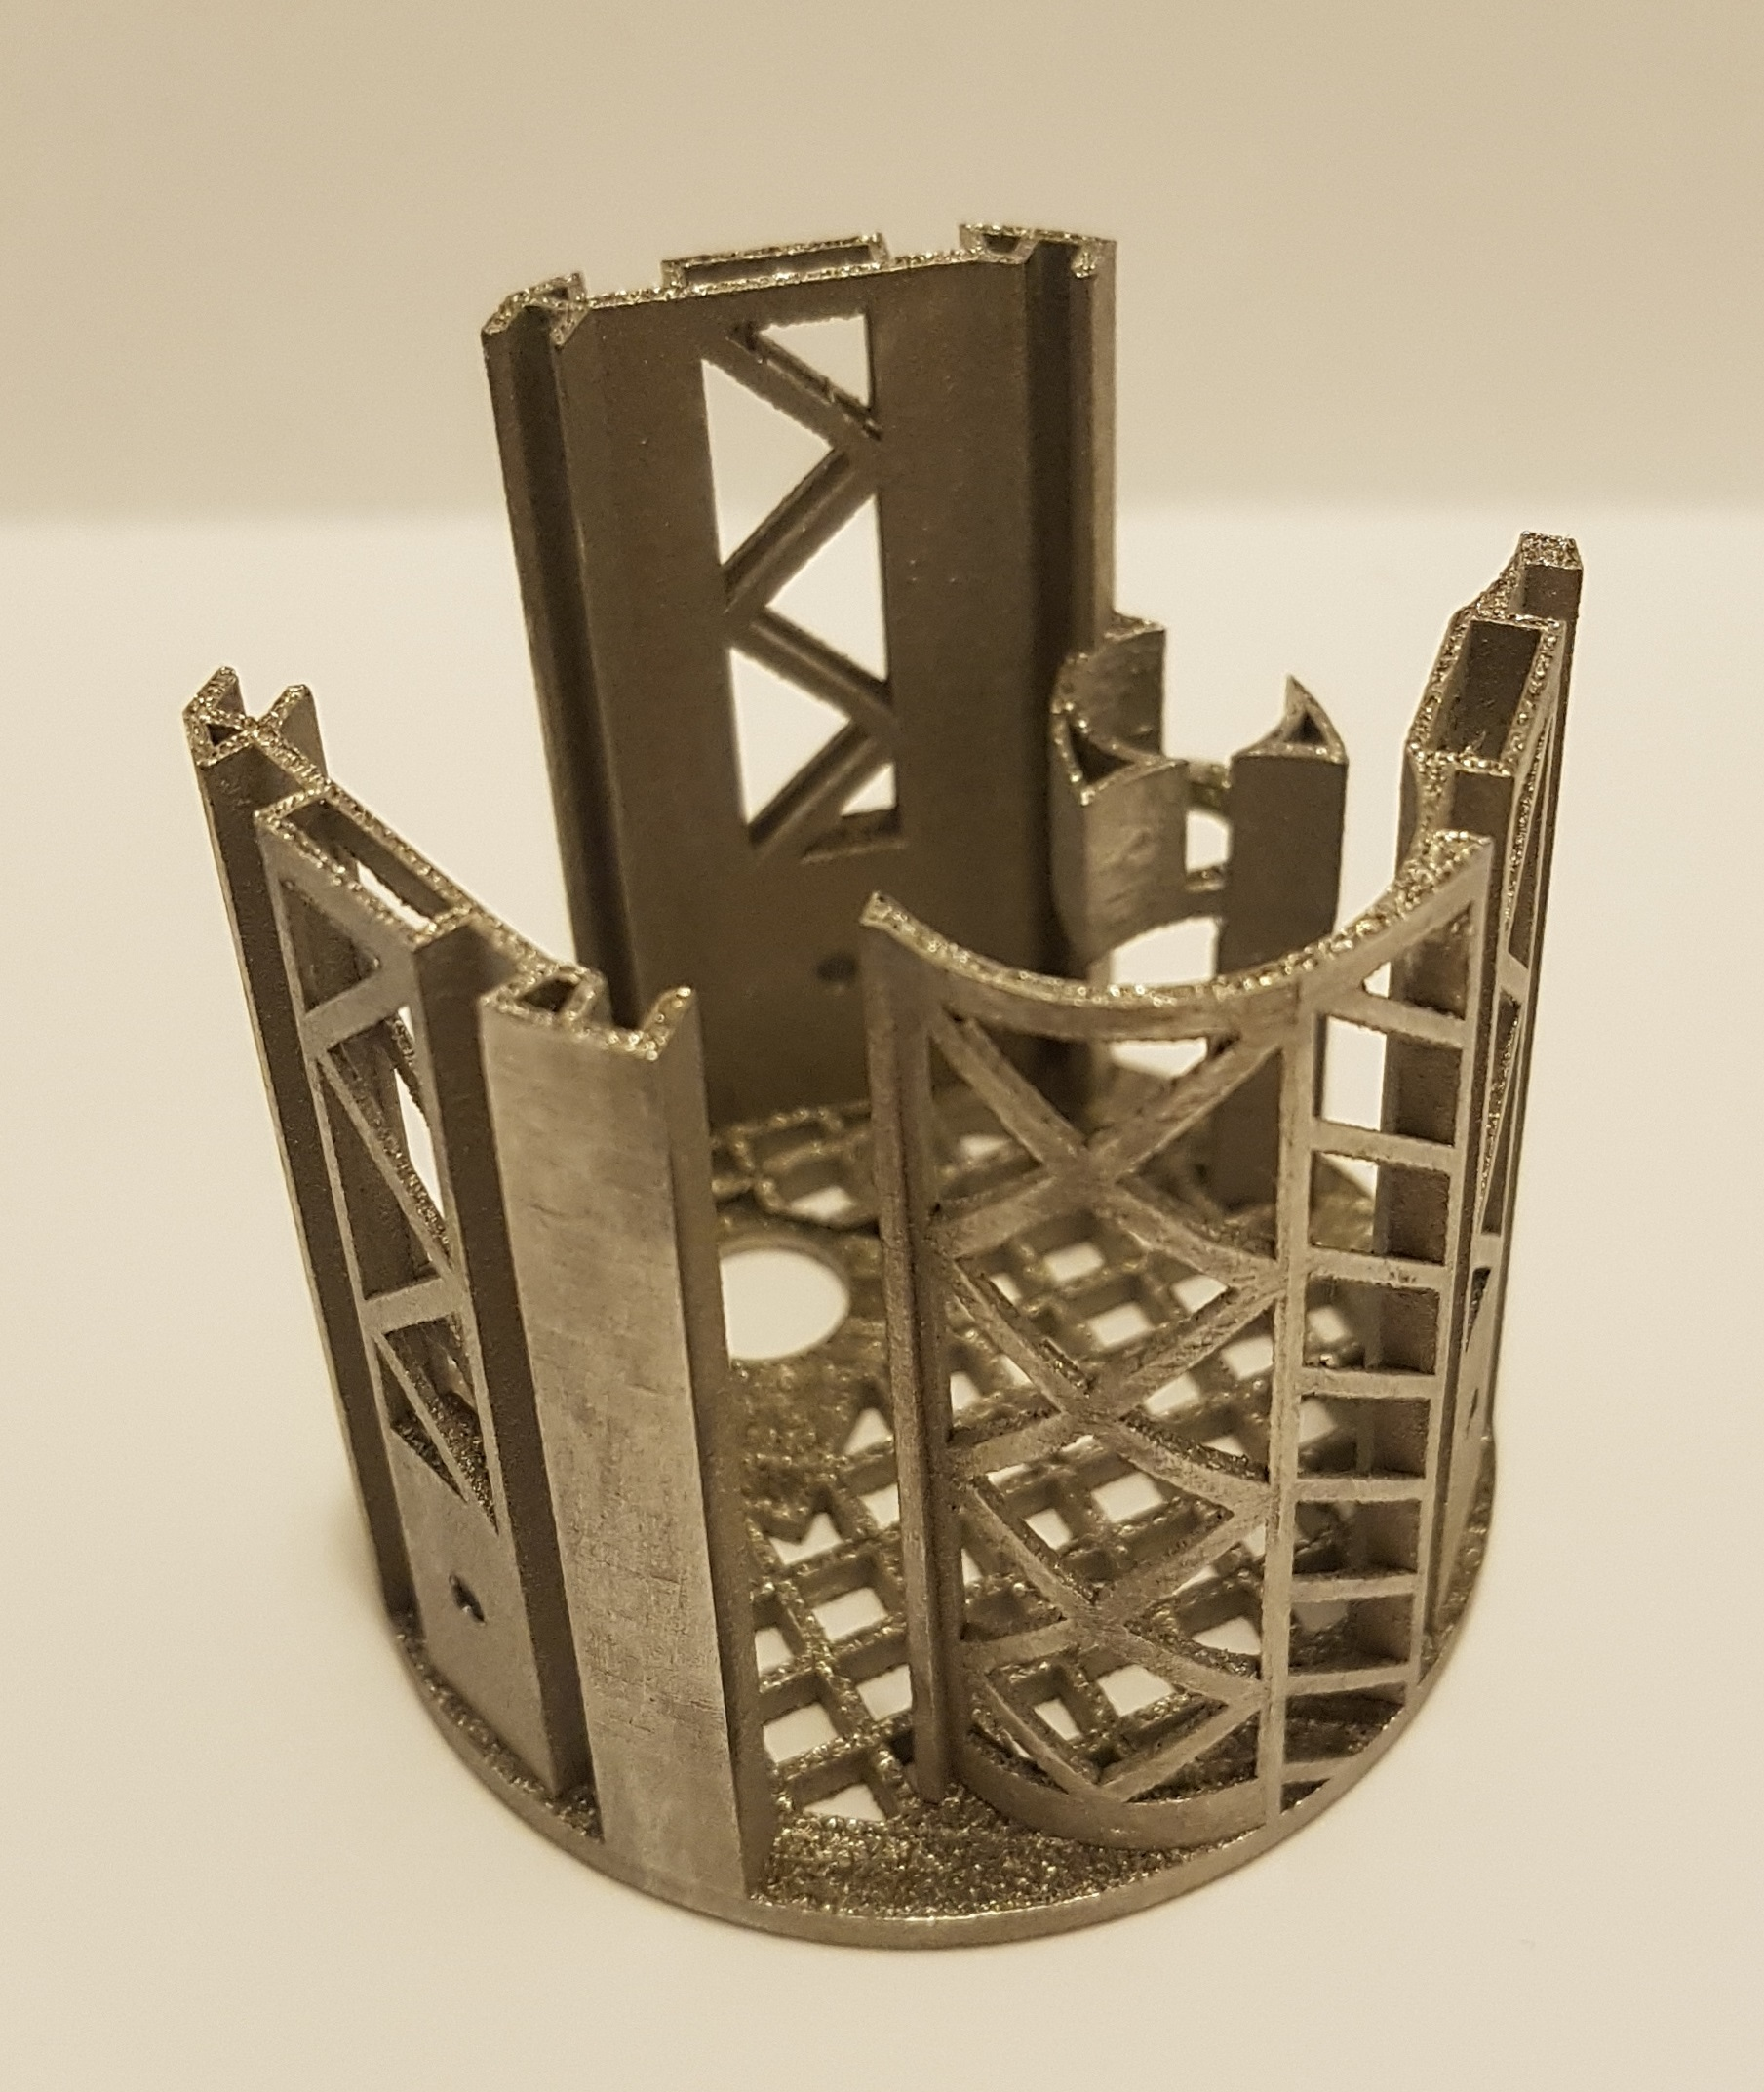
\includegraphics[scale=0.15]{steel_frame.jpg}\hspace*{\fill}
	\caption{A 3D printed steel CanSat bottom frame}
	\label{steelframe}
\end{figure}

This construction did allow for required tolerances but lead to near-maximum mass for the entire CanSat, preventing the team from pursuing any further add-on modules. A conductive steel frame also led to radio range reduction in our testing.

The team then ordered a nylon frame to be constructed via Shapeways again via SLS- this is shown in figure \ref{nylonframe}.

\begin{figure}[h]
	\hfill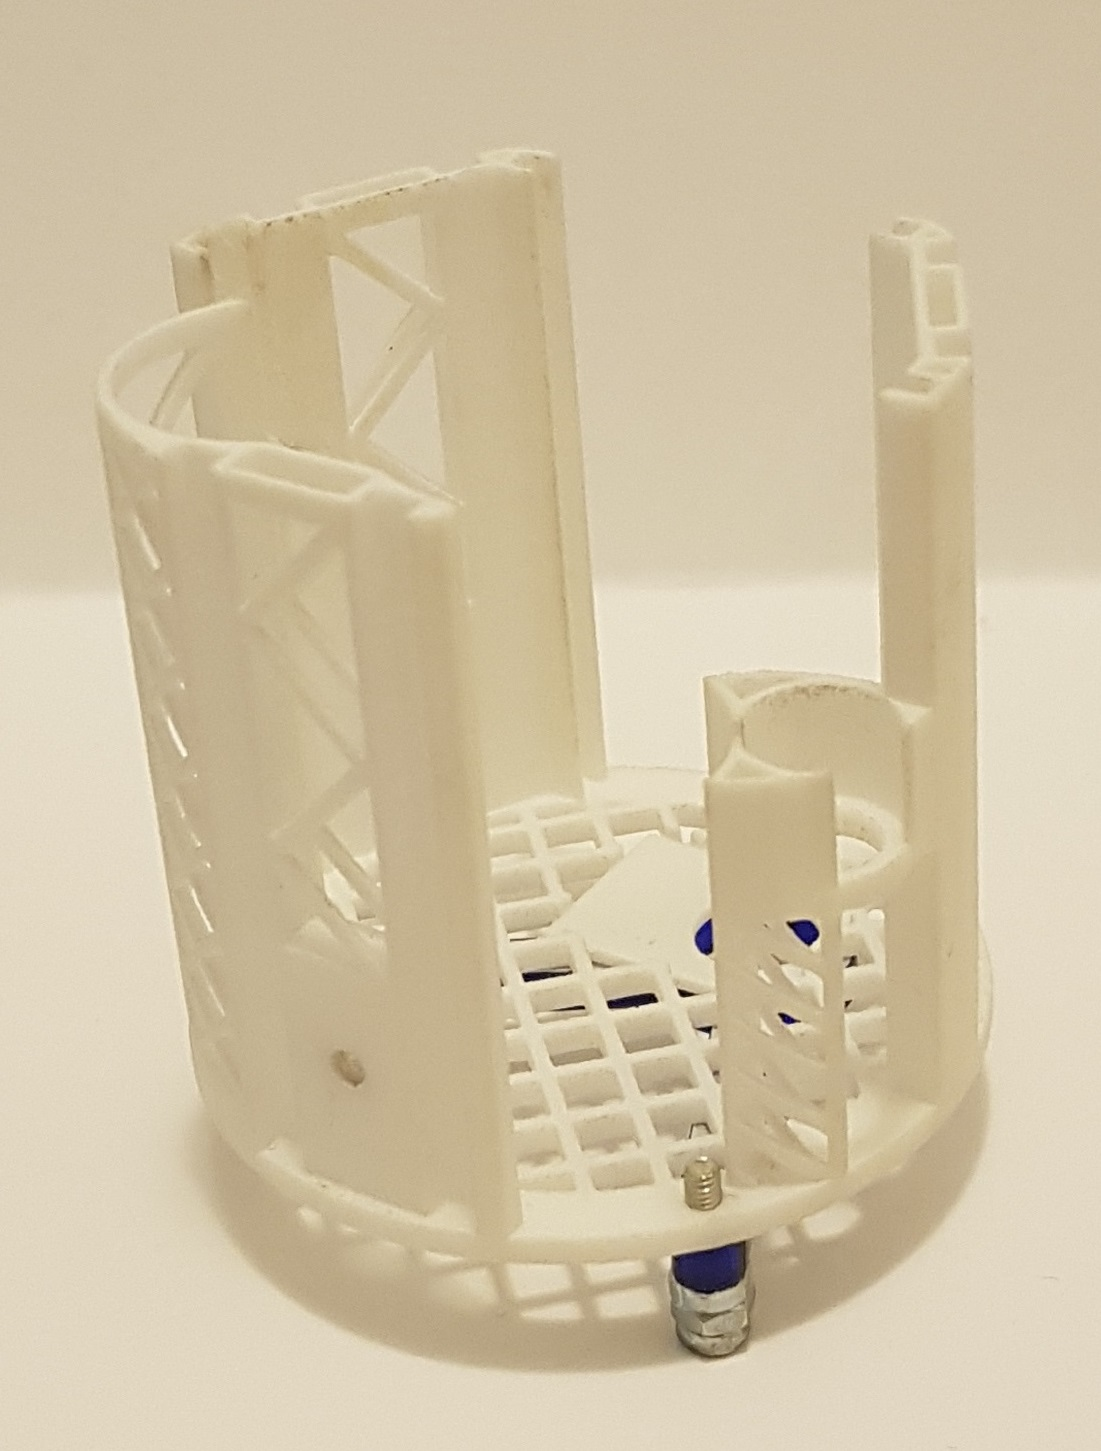
\includegraphics[scale=0.15]{nylon_frame.jpg}\hspace*{\fill}
	\caption{A 3D printed nylon CanSat bottom frame}
	\label{nylonframe}
\end{figure}

A nylon internal frame, while more flexible than desired, allowed for minimal weight while retaining the toughness and tolerances that our design required while remaining suitably affordable. In order to minimize the flexibility of the internal frame, the team has decided to use a steel top frame paired with a nylon bottom frame.
\subsection{Outer Shell}
\subsubsection{Prototype Design}
The team experimented with both 3D printed PLA and fiberglass in the creation of our outer shell. We found PLA to lack strength, easily cracking on impacts, while fiberglass proved to be a difficult material to acquire desired tolerances.

For our prototype outer shell, the team decided to use fiberglass molded around a bottle of the required diameter. The shell was then cut to size and provided with team and sponsor logos, protected with a transparent plastic sheet. An image of the prototype CanSat and outer shell can be seen in \ref{cshell}. 

\begin{figure}[h]
	\hfill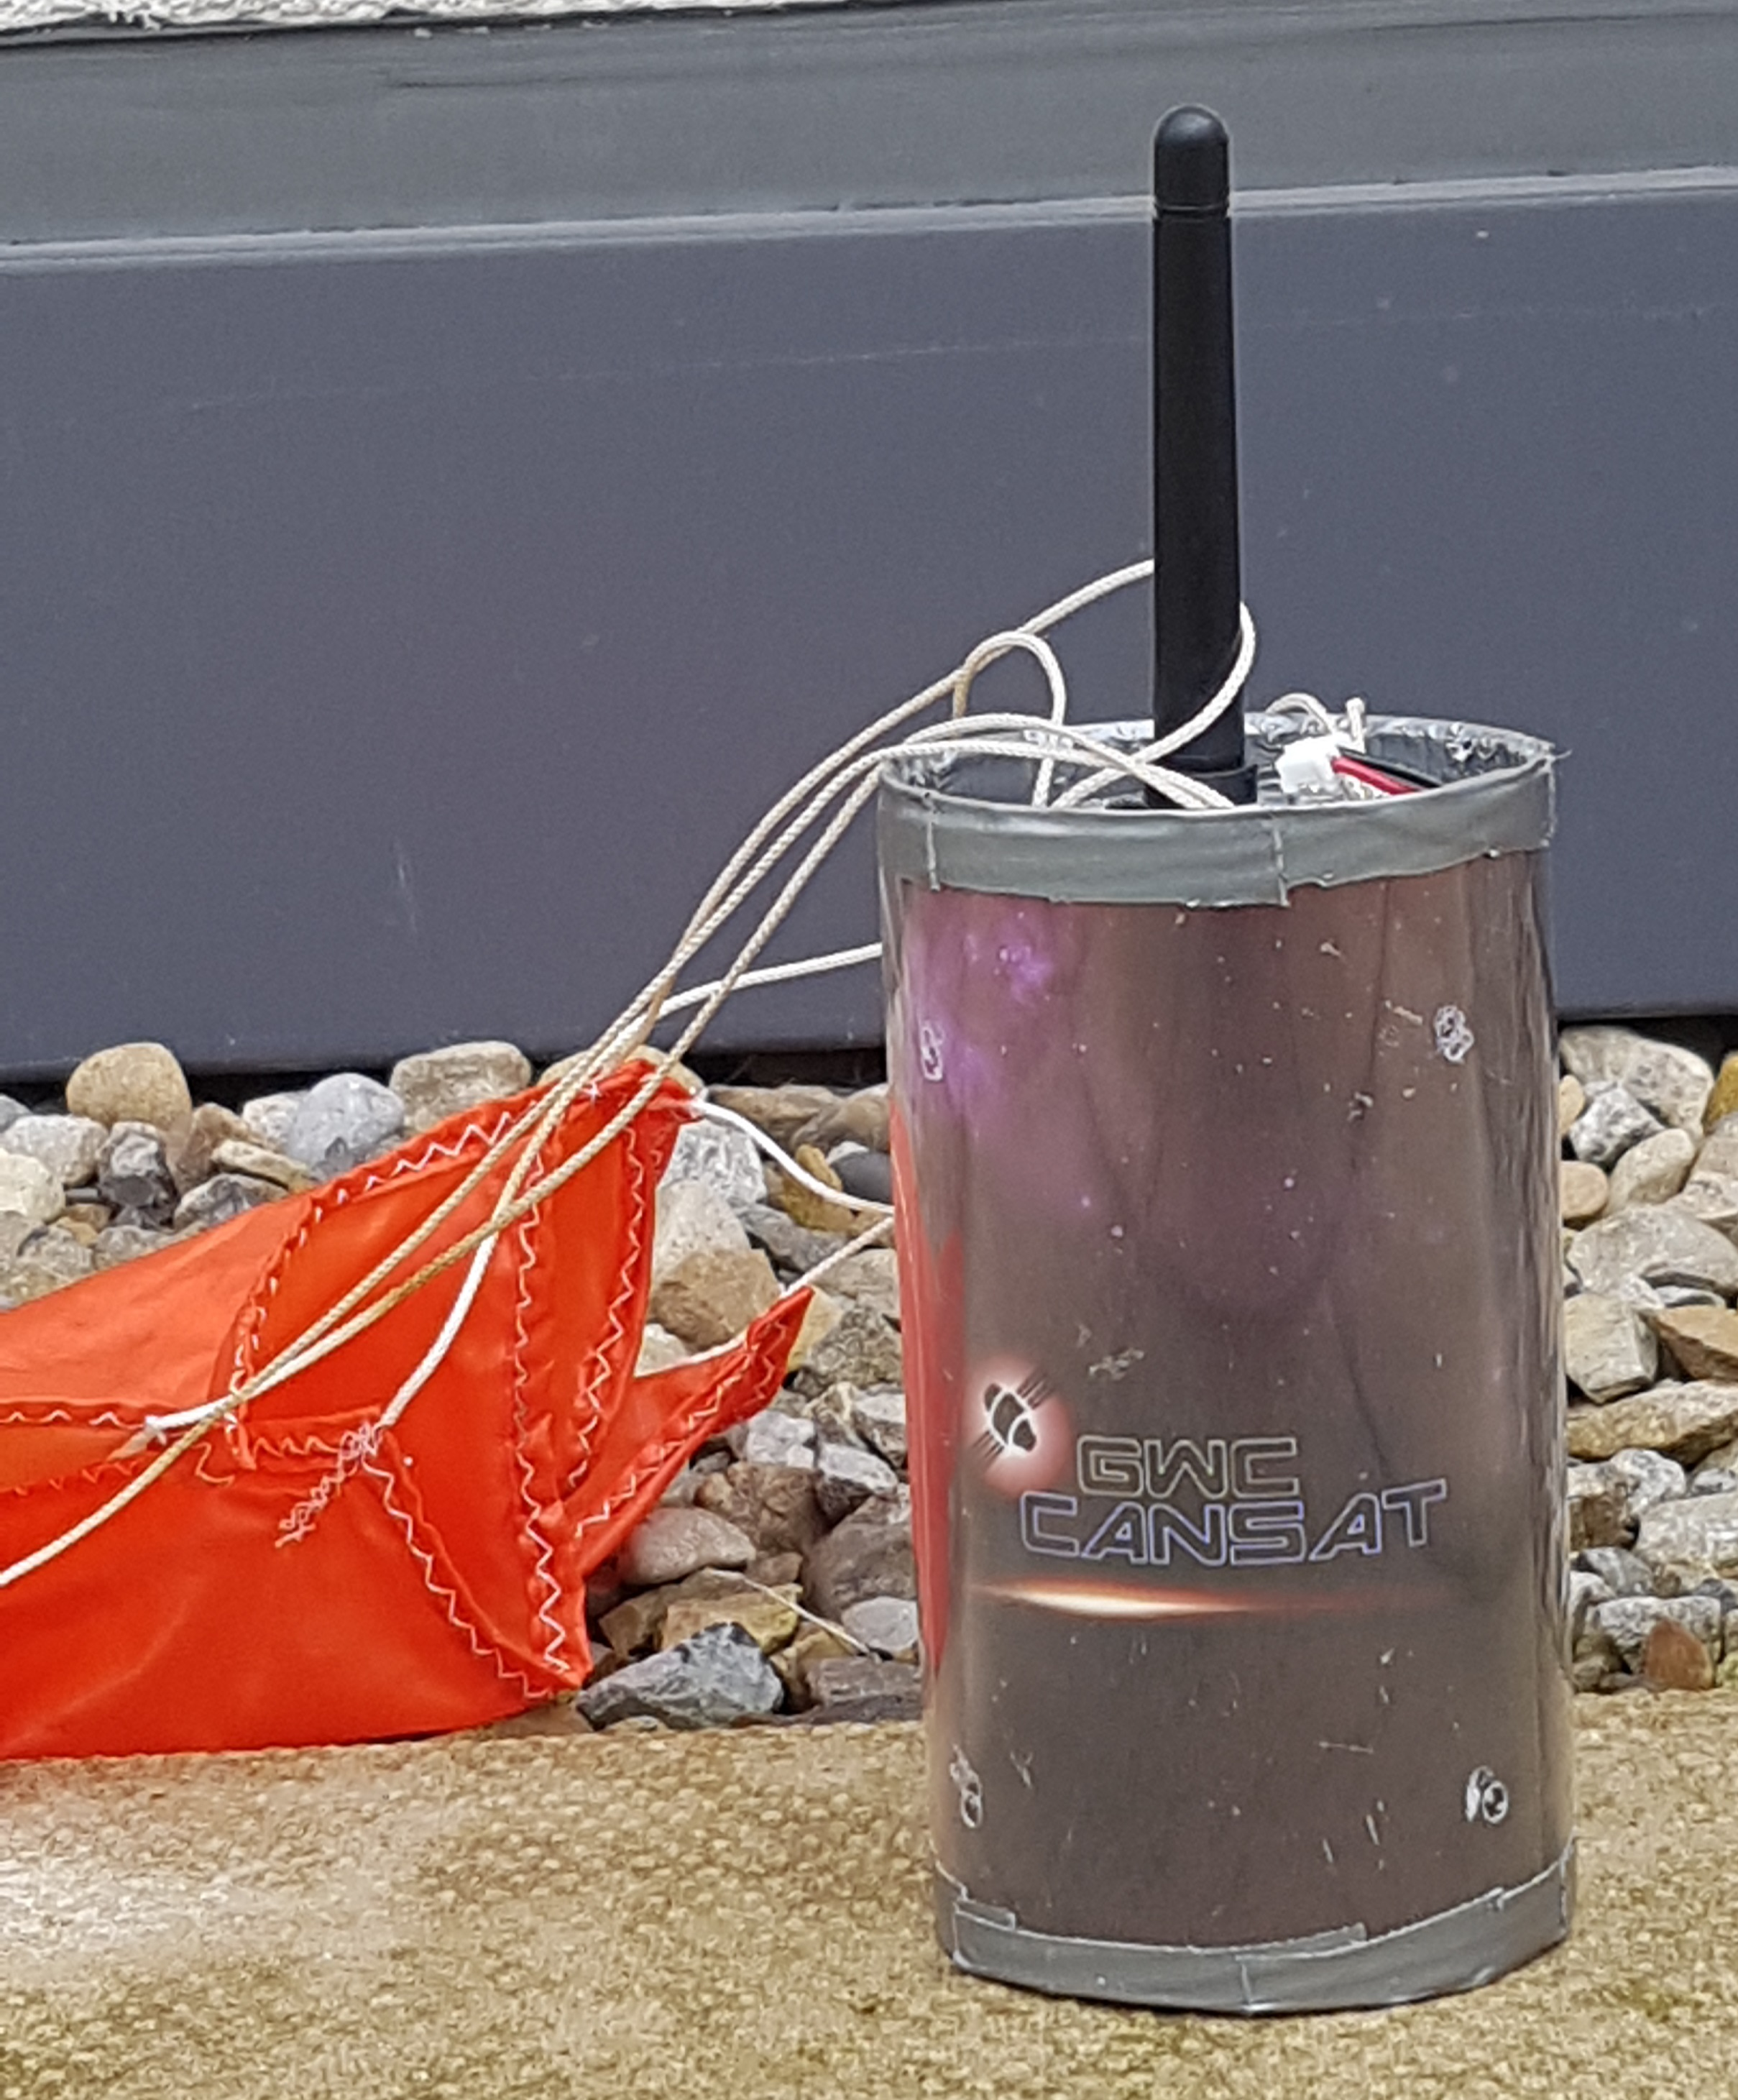
\includegraphics[scale=0.1]{cansat-shell.jpg}\hspace*{\fill}
	\caption{The prototype CanSat installed in the outer shell}
	\label{cshell}
\end{figure}


Spring steel mounts with screw plungers on the internal frame meshed with holes in the outer shell. This design, while offering further shock resistance via the spring steel, created difficulties when removing the internal frame from the outer shell.
\subsubsection{Final Design}
The team again elected to use a fiberglass outer shell. In order to improve tolerances, a mold was 3D printed out of PLA and covered with aluminum foil before the casting process began- the mold and a shell are visible in figure \ref{shellmold}.

\begin{figure}
	\centering
	\begin{subfigure}{.5\textwidth}
		\centering
		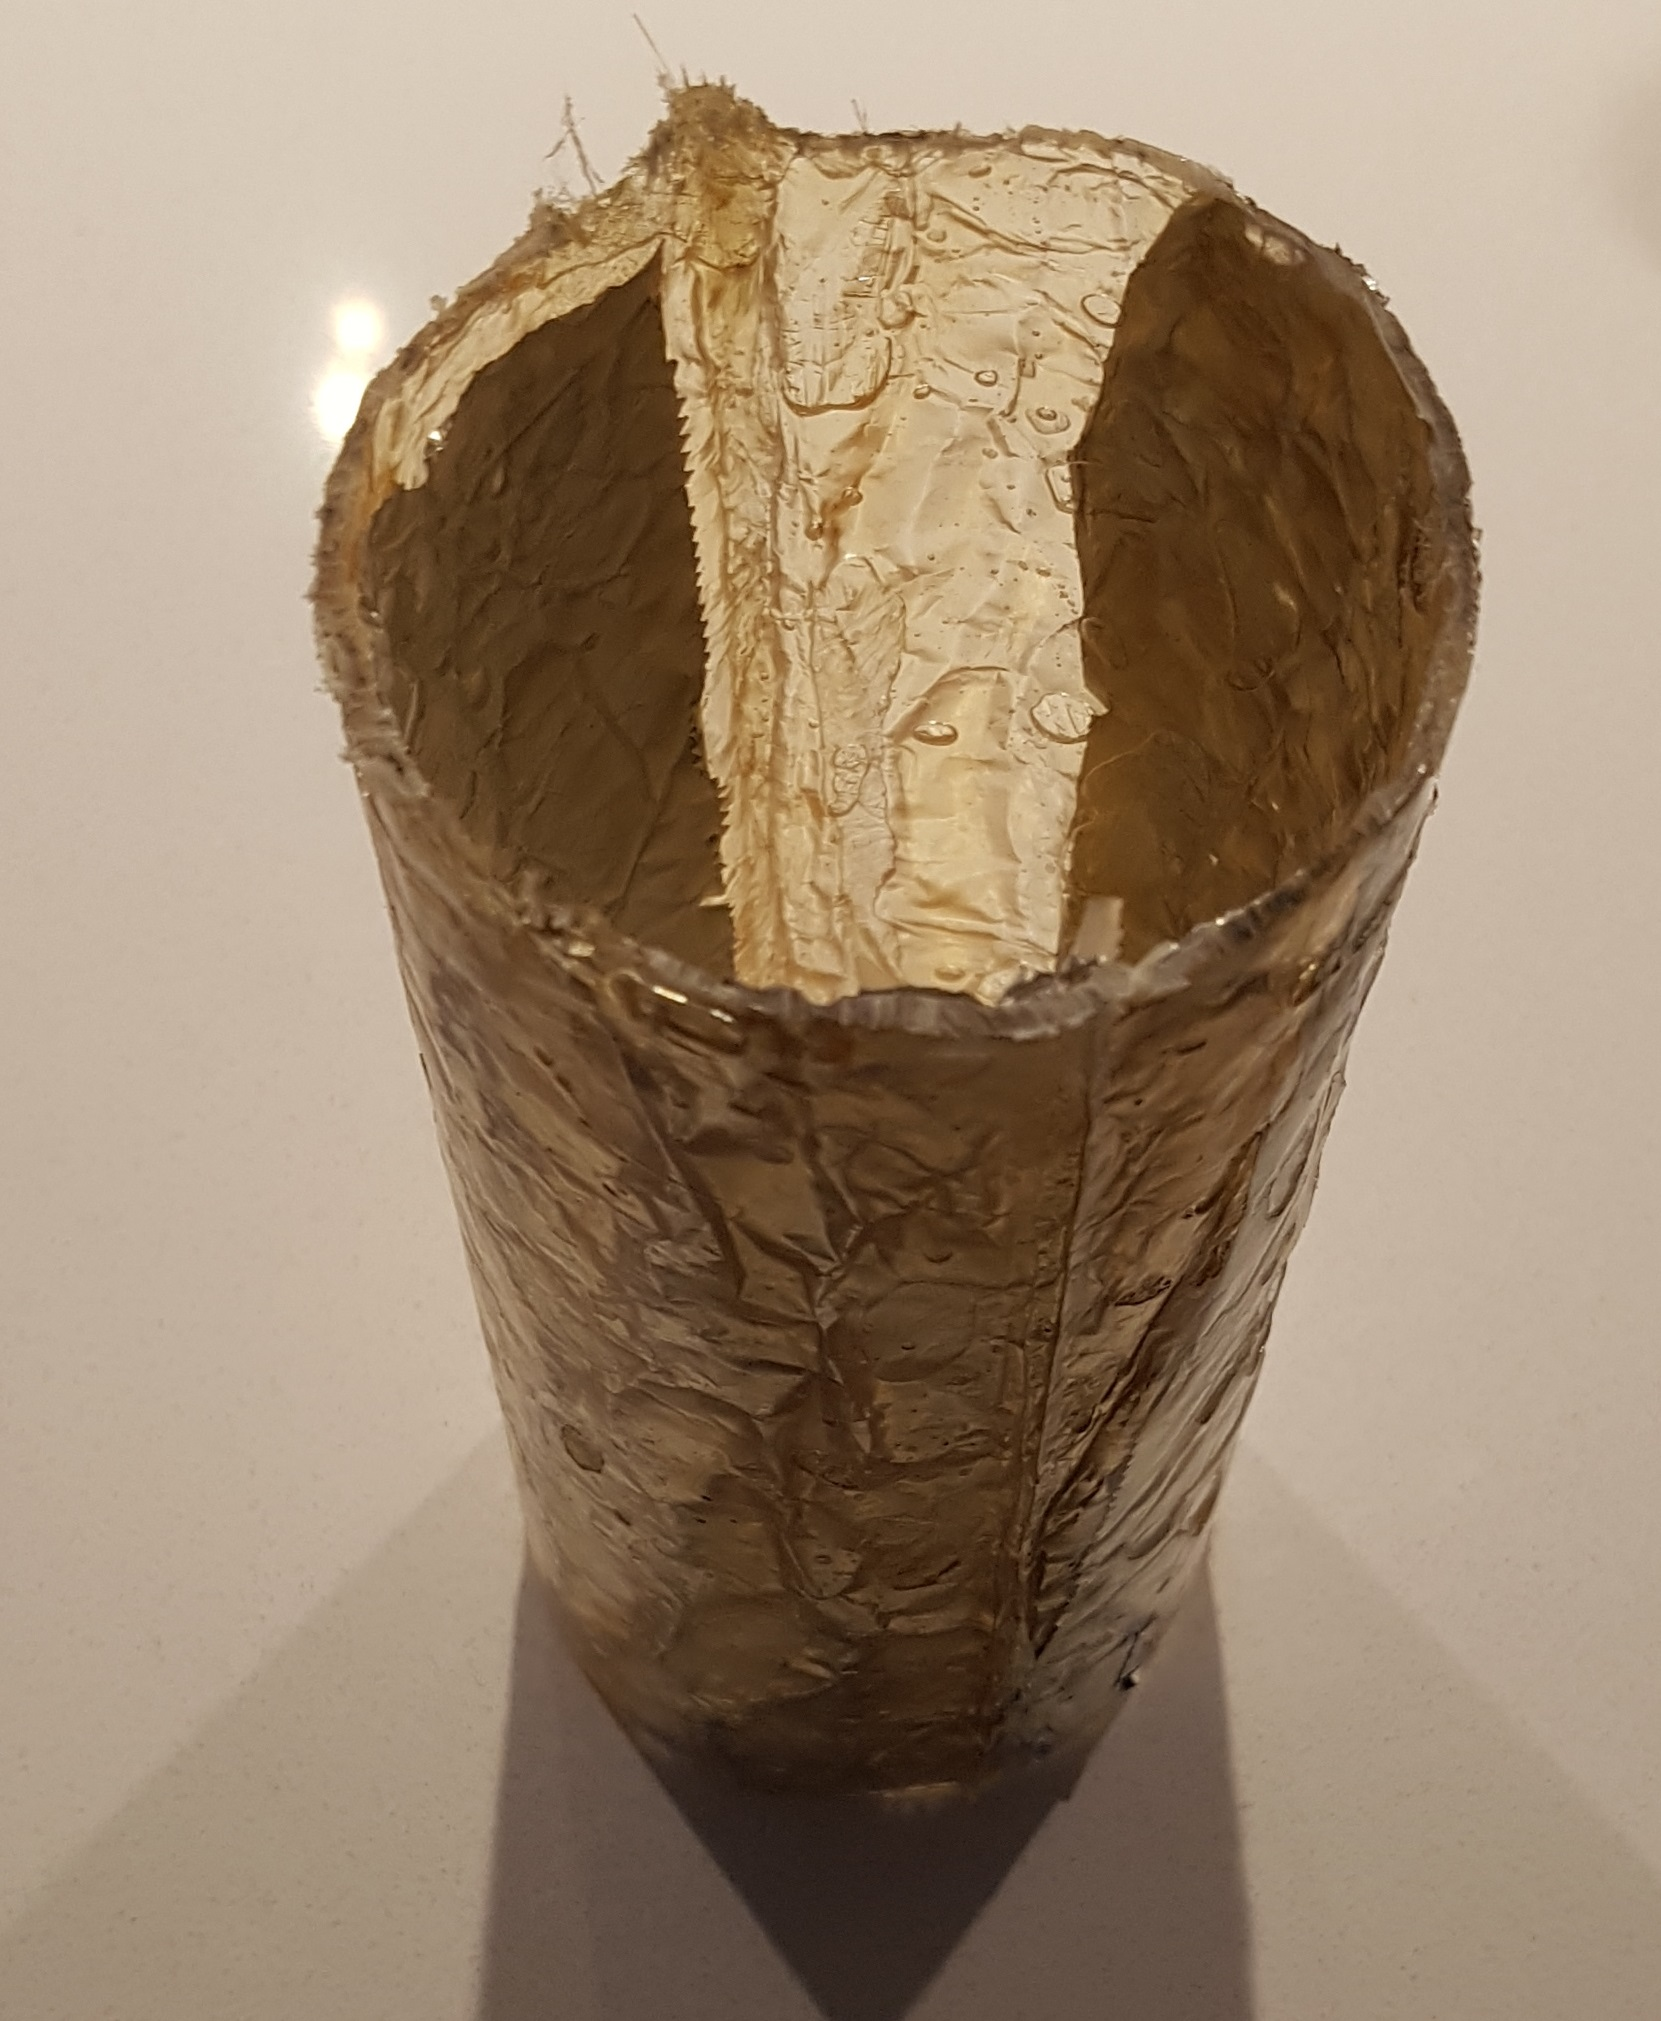
\includegraphics[width=.8\linewidth]{rawshell.jpg}
	\end{subfigure}%
	\begin{subfigure}{.5\textwidth}
		\centering
		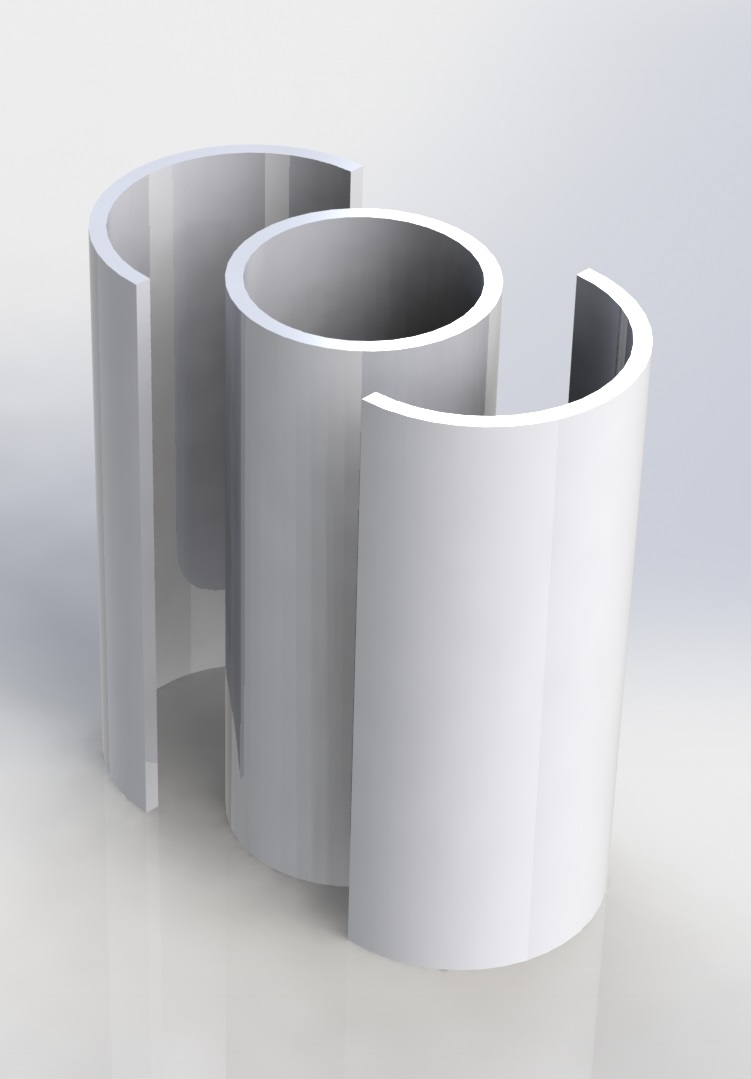
\includegraphics[width=0.7\linewidth, angle=0]{Mold_render.jpg}
	\end{subfigure}
	\caption{A raw outer shell with a render of its mold}
	\label{shellmold}
\end{figure}

In order to minimize the mounting difficulties found in the CanSat prototype, the team decided on a slider system built from 3D printed PLA to allow for outer shell – internal frame mounting, secured via a set of bolts. This mechanism is visible in figure \ref{sliders}. While this system would lack the shock resistance of the CanSat prototype the team believed it to be a worthwhile tradeoff. 

\begin{figure}
	\centering
	\begin{subfigure}{.5\textwidth}
		\centering
		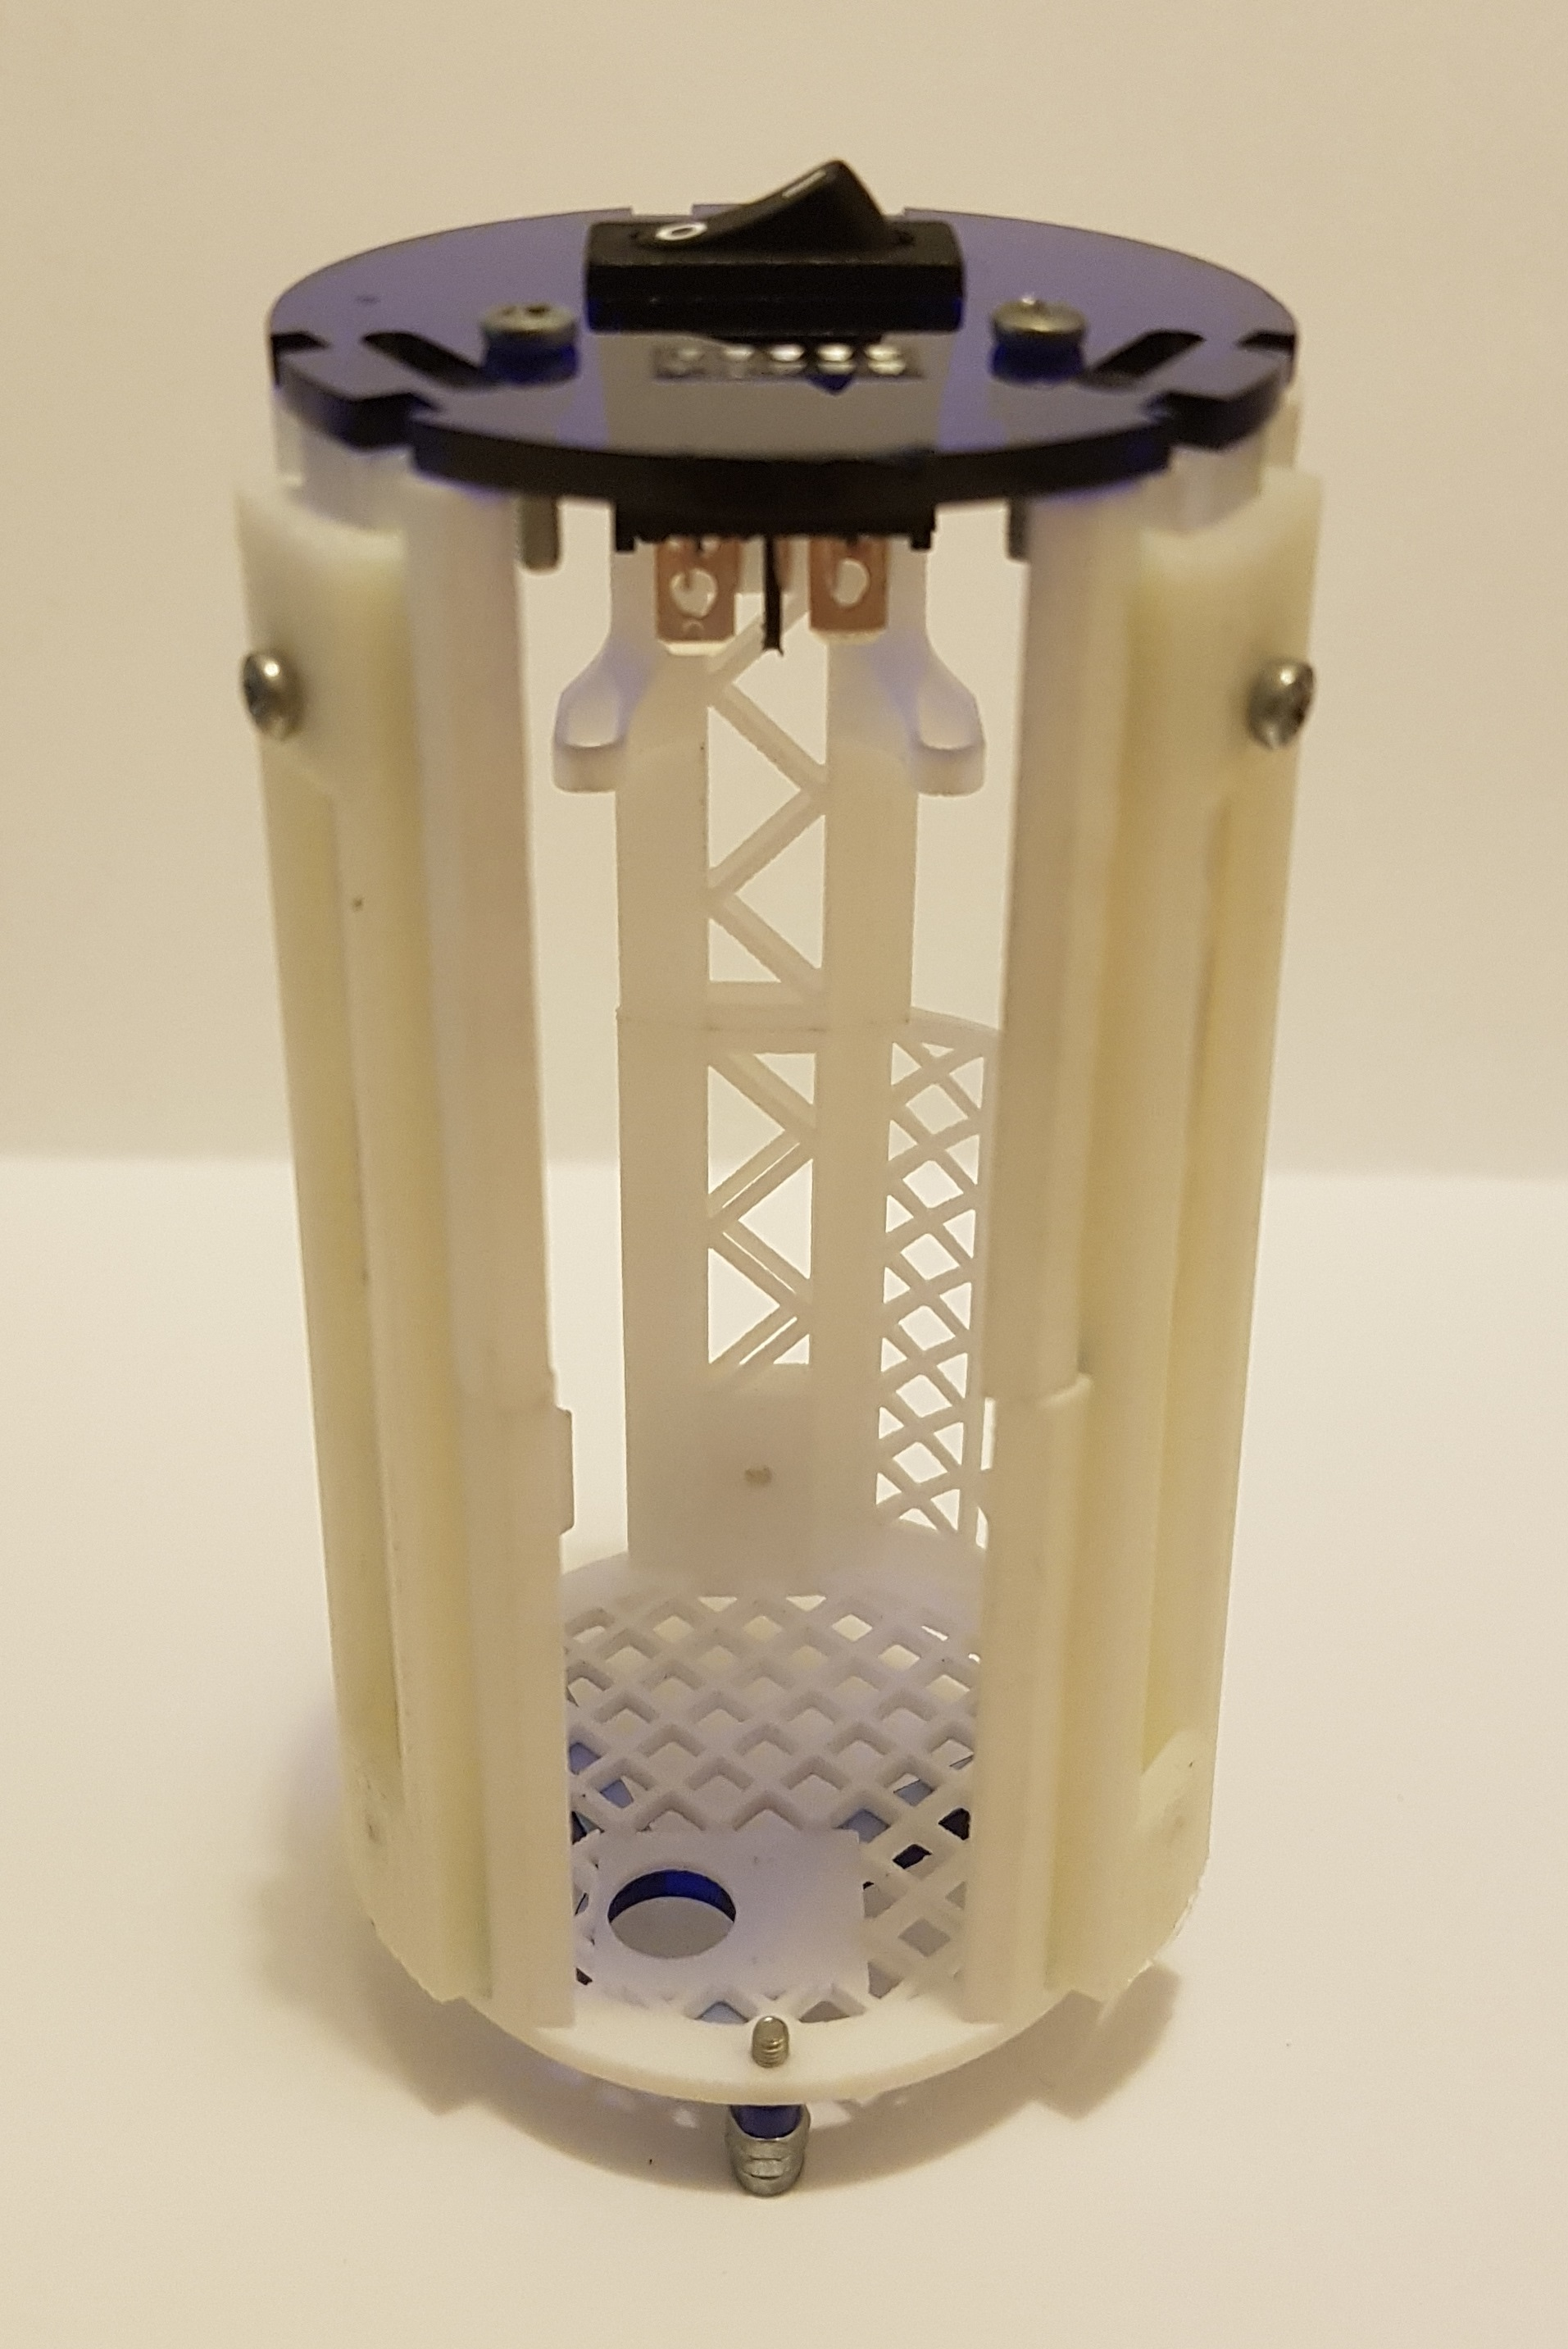
\includegraphics[width=.7\linewidth]{bareframe.jpg}
	\end{subfigure}%
	\begin{subfigure}{.5\textwidth}
		\centering
		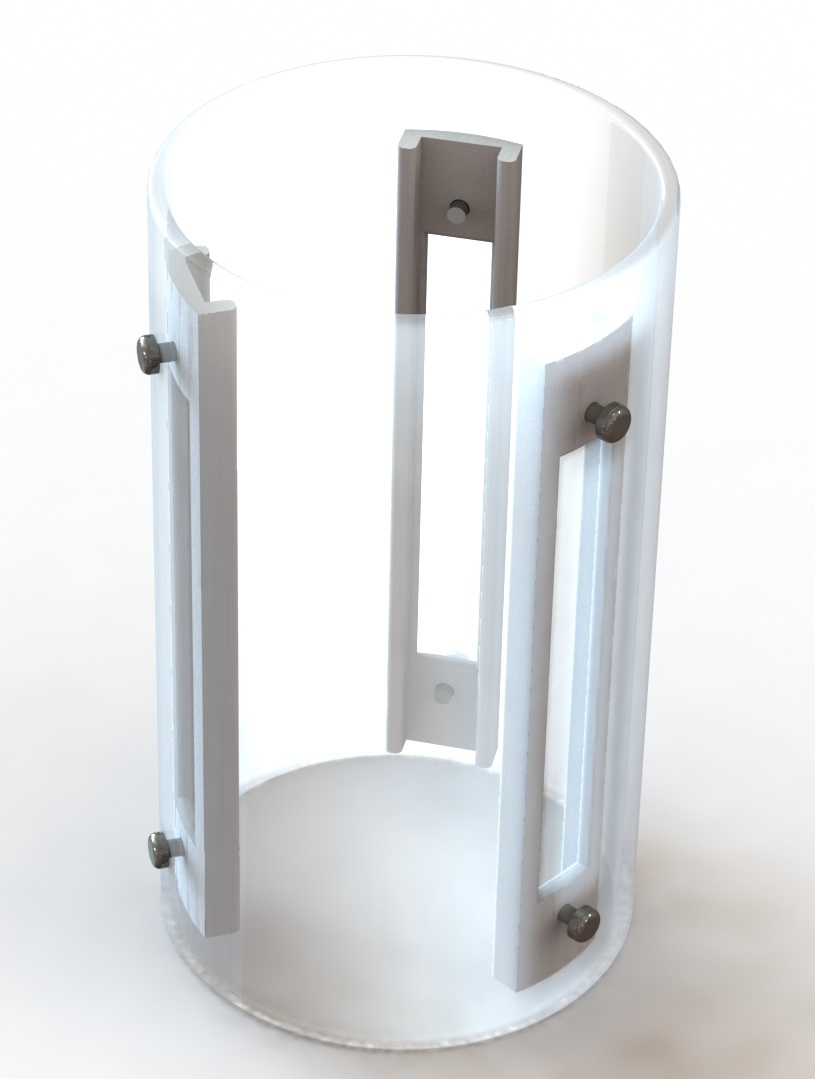
\includegraphics[width=0.8\linewidth, angle=0]{Outer_shell_render.jpg}
	\end{subfigure}
	\caption{The CanSat slider mechanism}
	\label{sliders}
\end{figure}

\subsection{Electronics}
\subsubsection{Prototype Design}
In the team brainstorming session, we decided to mount all sensors and electronics to a vertical PCB or protoboard. While a set of vertically stacked, circular electronics boards would theoretically provide more surface area, no single board would provide enough space for the single-board-computer and batteries that we aimed to use. Additionally, a single electronics board would facilitate assembly and reduce the number of points of failure. In order to provide long battery runtimes, the team also planned to include a pair of 2200mAh lithium-ion cells in the 18650 form factor. The relatively large size of these cells led to a press-fit mount as seen in figure \ref{emount}.

\begin{figure}[h]
	\hfill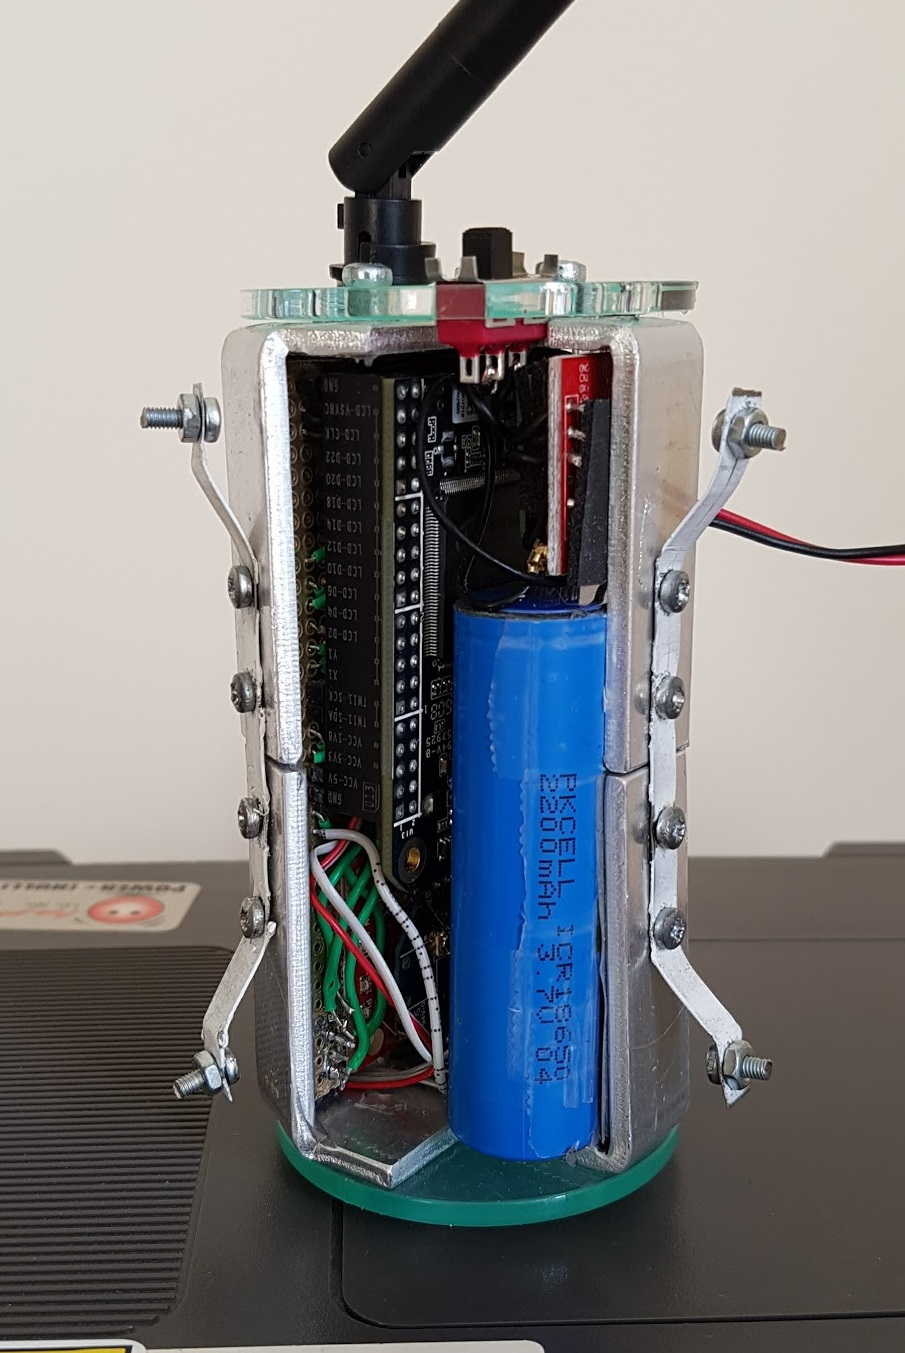
\includegraphics[scale=0.4]{old_cansat_side.jpg}\hspace*{\fill}
	\caption{Electronics mount on the prototype CanSat}
	\label{emount}
\end{figure}

The thermal camera was placed at the bottom of the CanSat, against the steel frame, and the cellular GSM module was secured via adhesive above the battery. An annotated image of the prototype CanSat can be seen in figure \ref{anoldcan}.

\begin{figure}[h]
	\hfill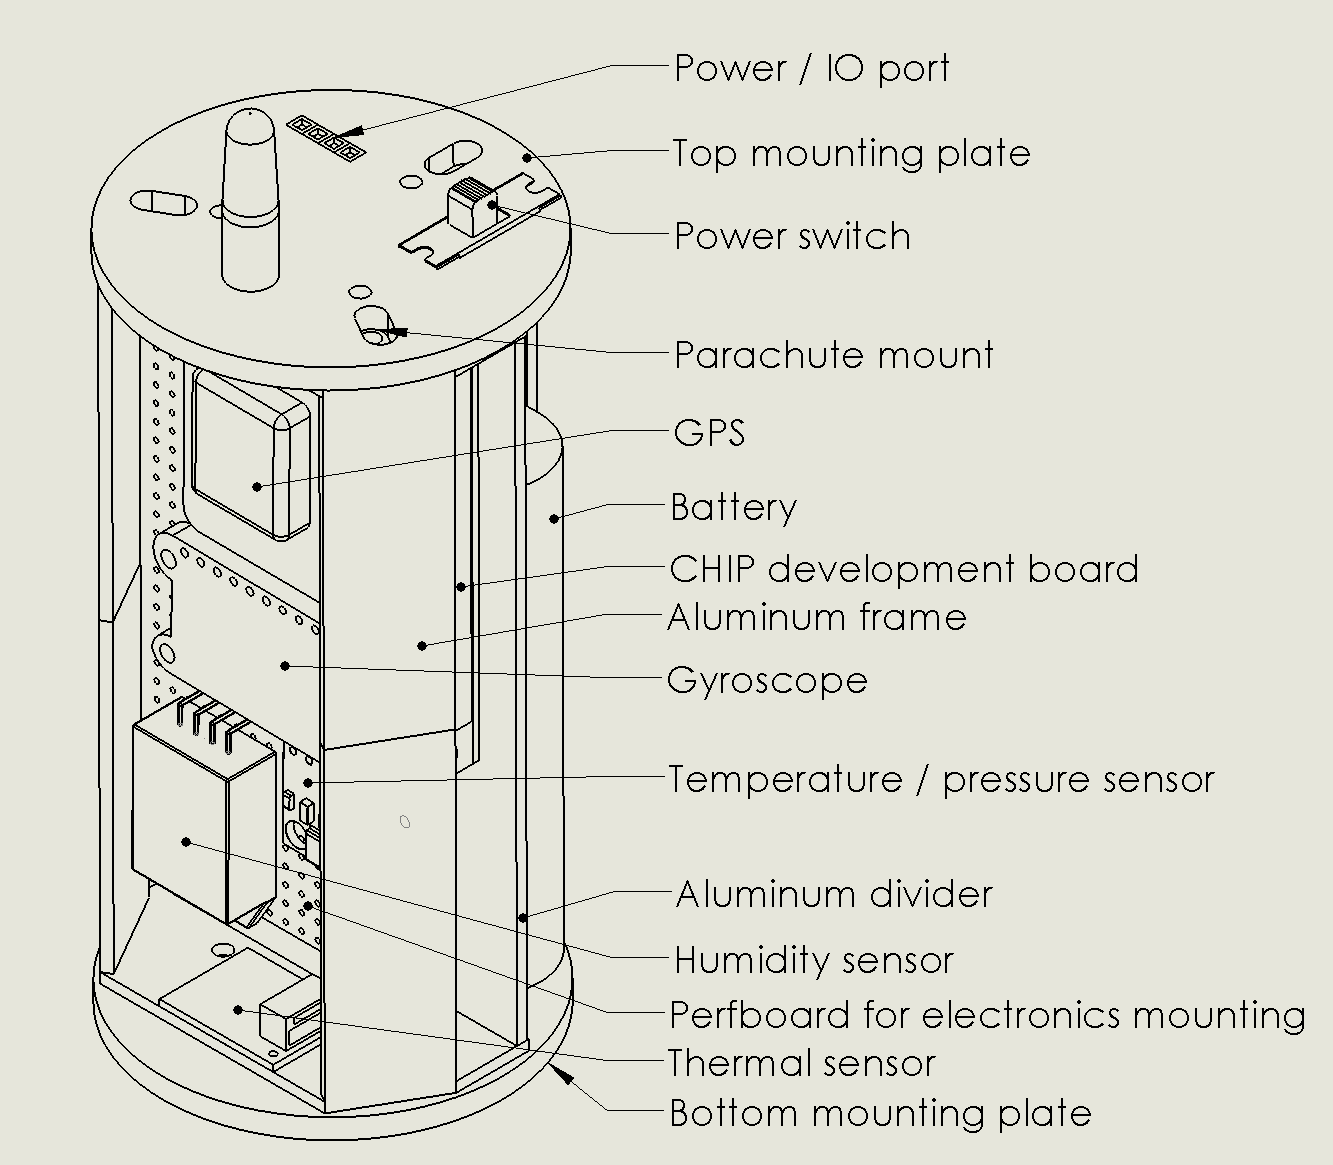
\includegraphics[scale=0.2]{annotated_cansat.png}\hspace*{\fill}
	\caption{An annotated view of the prototype CanSat}
	\label{anoldcan}
\end{figure}

\subsubsection{Final Design}
The team maintained a similar sensor payload in the second CanSat revision, although the use of new sensors allowed us to condense the pressure and humidity sensors into one unit. A more advanced internal frame design also allowed for easier and more secure battery and electronics mounting, illustrated in figure \ref{elecmount}.

\begin{figure}[h]
	\hfill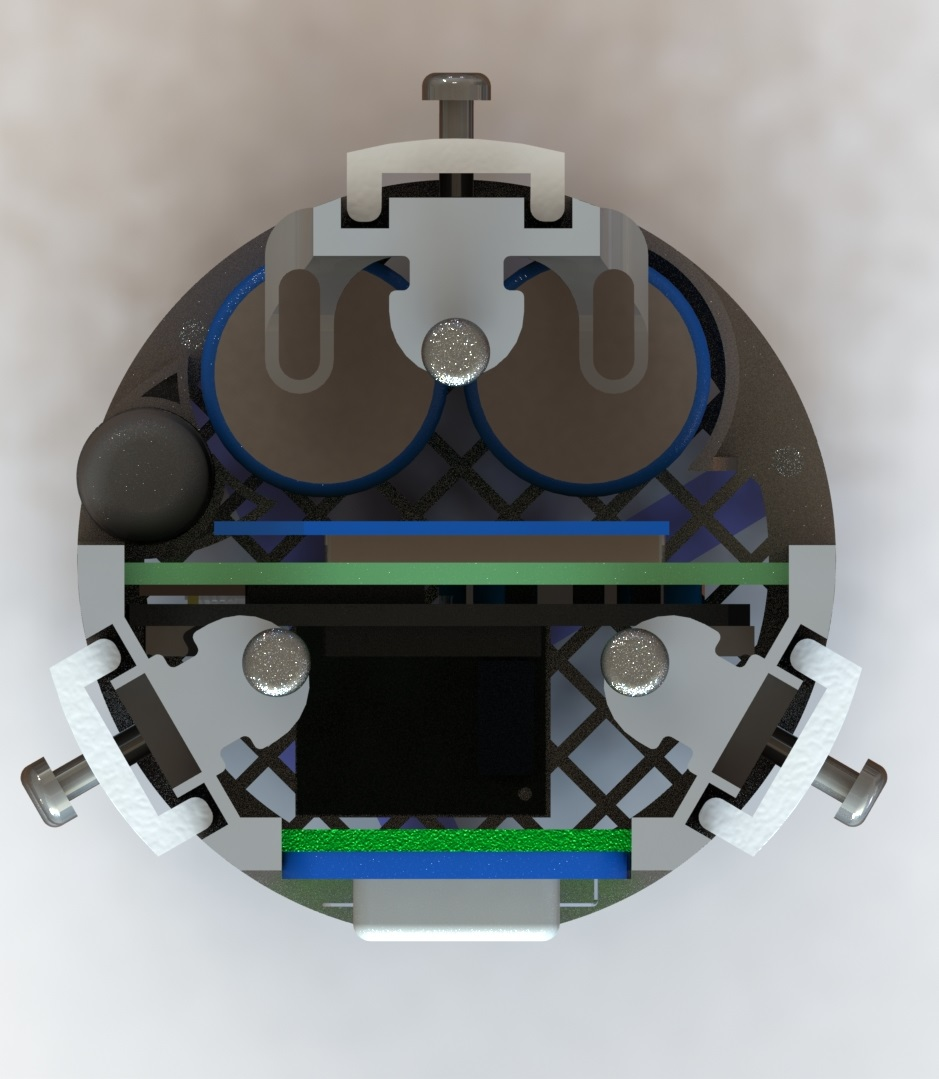
\includegraphics[scale=0.5]{electronics_mount_render.jpg}\hspace*{\fill}
	\caption{A render illustrating electronics mounting in the final CanSat}
	\label{elecmount}
\end{figure}

\section{Electrical Design}
\subsection{Sensor and Device Wiring}
\subsubsection{Prototype Design}
Similar to the section describing the mechanical design, the team's experiences in our prototyping phase provide context to our design decisions in our final CanSat design.

Throughout our CanSat brainstorming, prototyping, and final design, the team used a Linux single-board-computer as the main control board in our CanSat. One of our team's objectives was for the CanSat to stay relatively independent of the base station- to be able to do all sensor processing on-CanSat, to compensate for any electrical, radio, or hardware failures, and, if necessary, for the base station to be able to alter CanSat code over a radio connection. These objectives required more computing power than was available in the eight-bit Atmel MCUs common in hobby development boards, so the team settled on a Linux SBC: the CHIP, designed by Next Thing Co, for our prototype design. The CHIP includes a 1GHz ARM CPU, 4GB of Flash, and 512MB of RAM. For this design, sensor payload was as seen in figure \ref{anoldcan}: 

The CHIP provided battery regulation and charging, as well as stable and high-current-capable 5V, 3.3V, and 1.8V rails. We experienced no issues powering sensors and radios, though logic level shifting circuitry was necessary for some sensors.

The team did struggle with serial I/O in our prototype design. The CHIP theoretically supports multiple serial ports, but the team was only able to interface with one port echoing the Linux console. Hence we added an Arduino Pro Mini to serve as a serial-I2C interpreter. 

Our prototype design saw these components wired to a single protoboard as seen in figure \ref{pboard}.

\begin{figure}[h]
	\hfill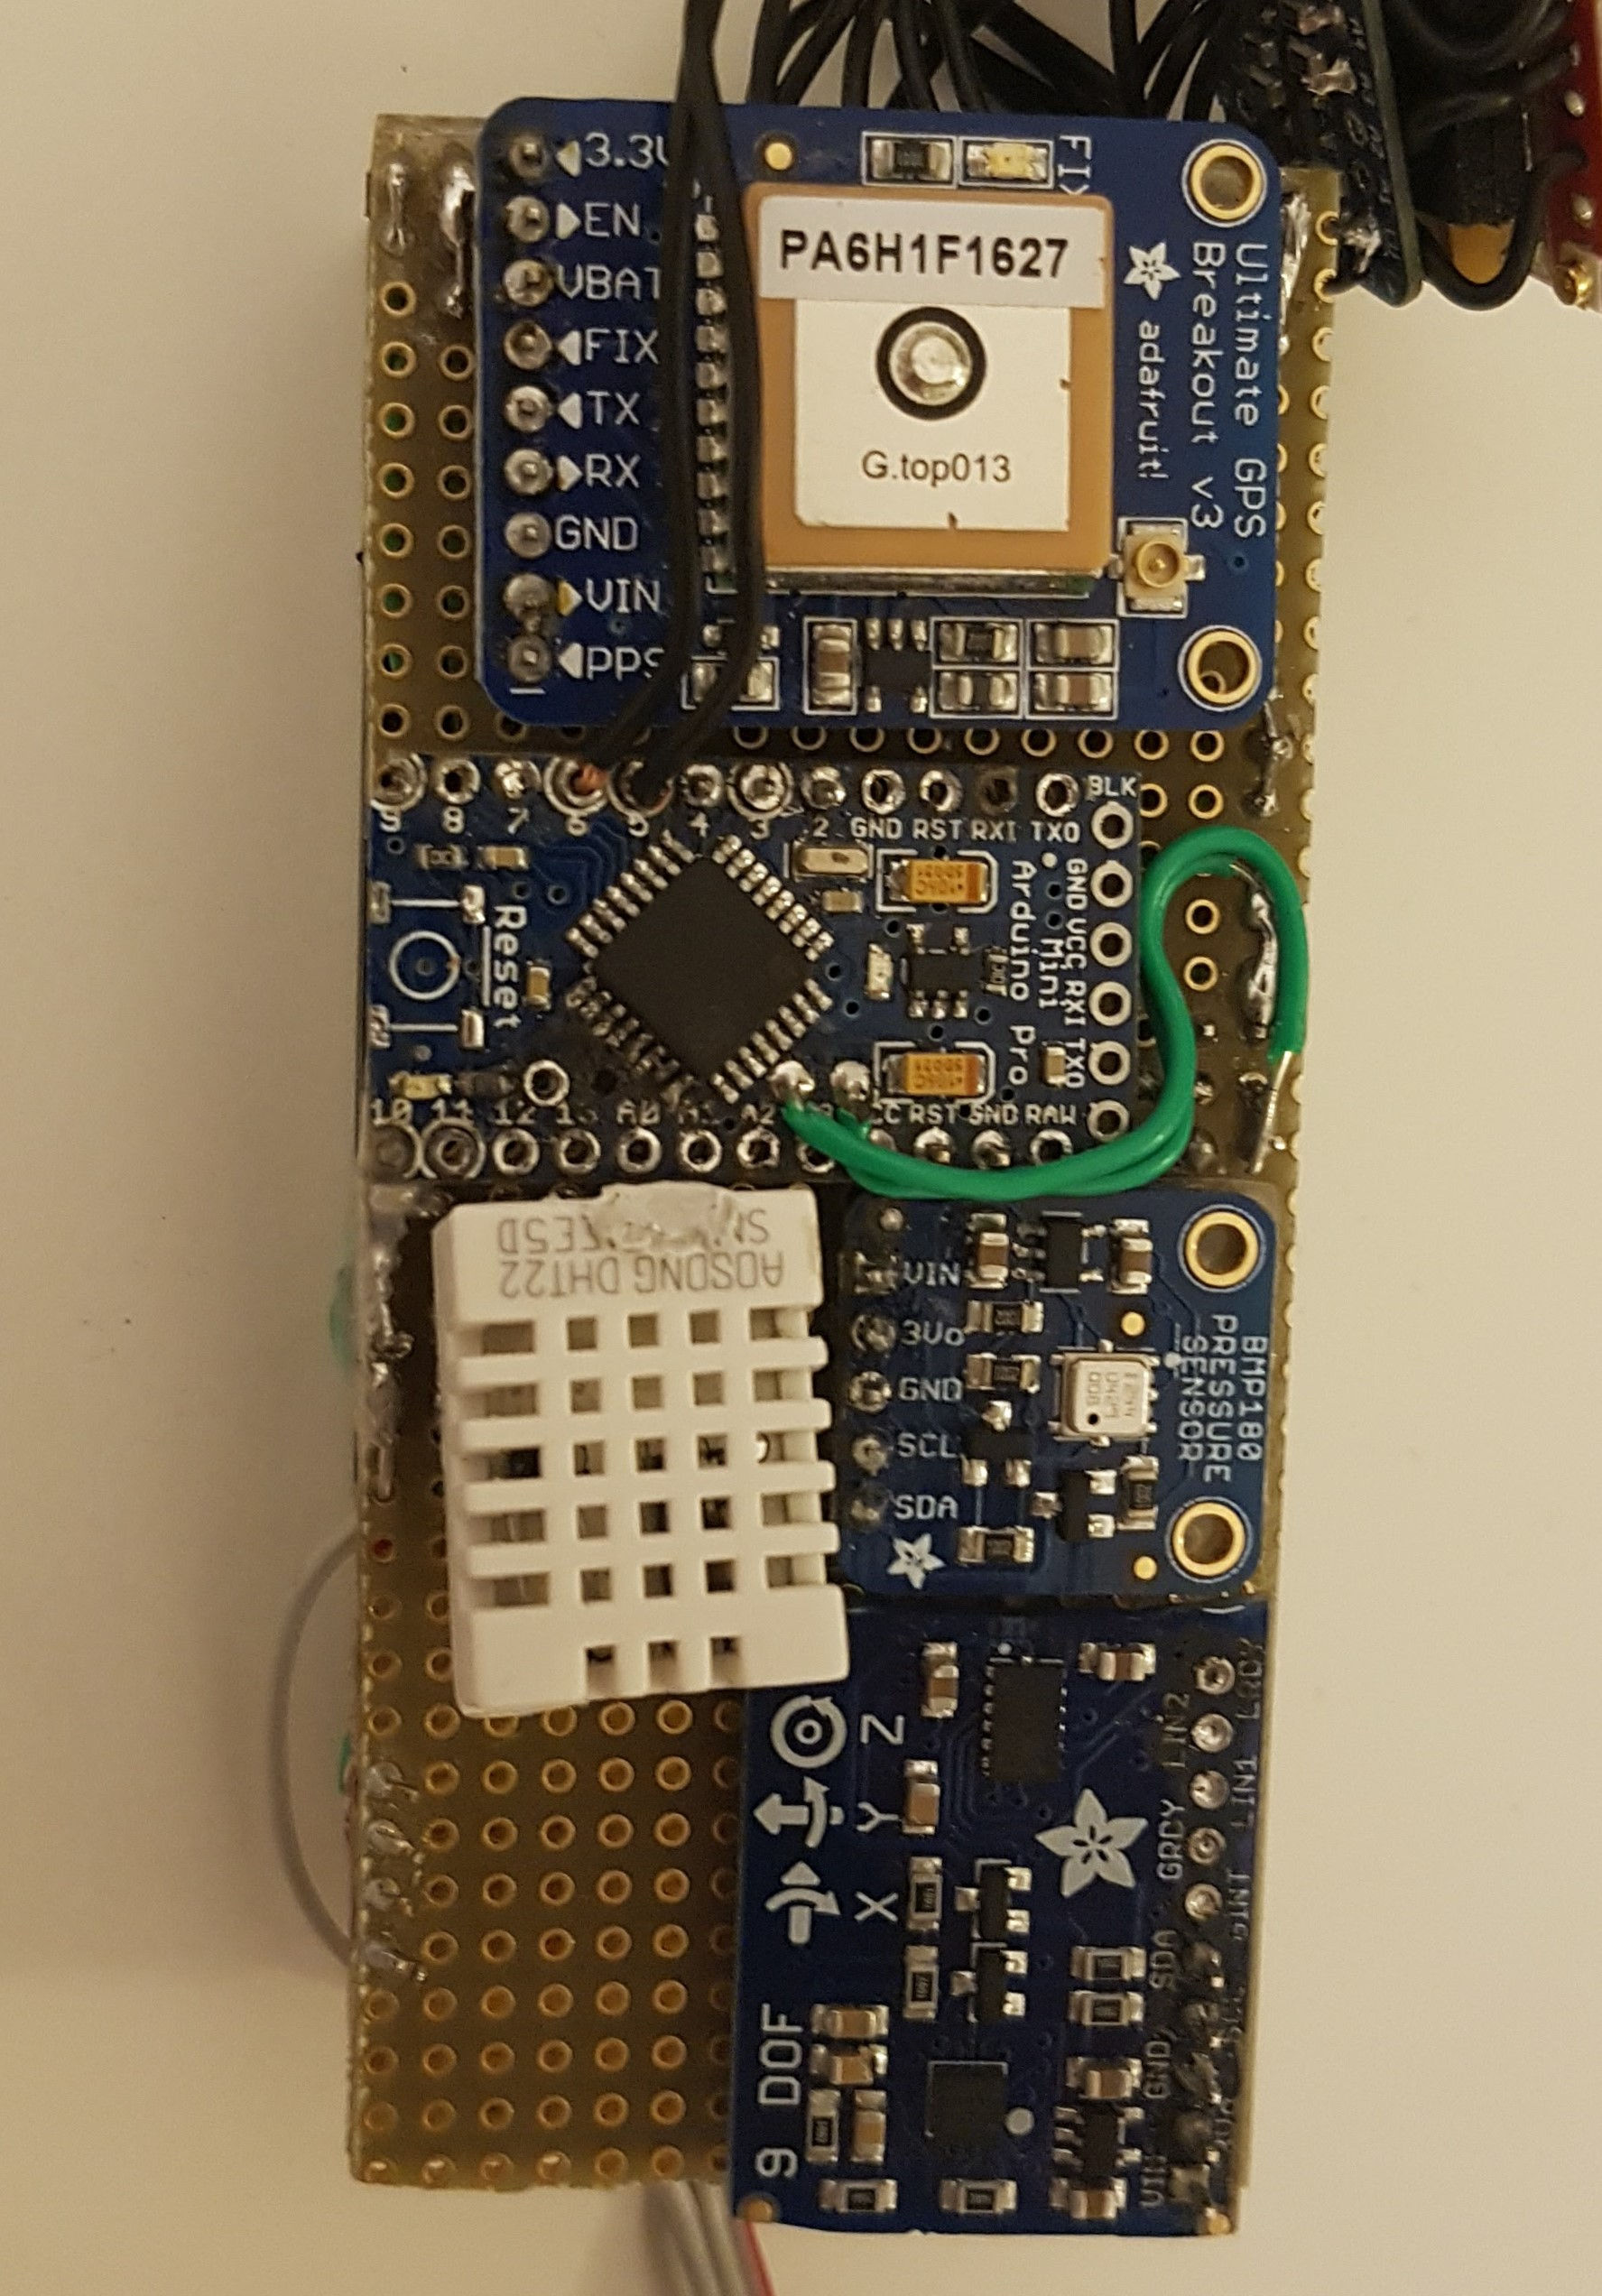
\includegraphics[scale=0.1]{protoboard.jpg}\hspace*{\fill}
	\caption{The prototype CanSat electronics board}
	\label{pboard}
\end{figure}

\subsubsection{Final Design}
As mentioned earlier, the electrical design remained relatively constant between revisions. The largest electrical change was in deciding to design custom PCBs to maximize available sensor mounting space, visible in figure \ref{pboardnew}. 

With custom PCBs, we were able to include surface mount components. This allowed us to mount supporting GPS, XBEE, and level shifting circuitry directly on the PCB, removing the need for expensive breakout boards. We also decided to use the CHIP Pro instead of the CHIP: while it only included 512MB of Flash and 256MB of RAM, it promised lower power consumption and a PCB friendly footprint. We also used a BME280, replacing the DHT22 and BMP180, and offering humidity, pressure, and temperature sensors.

Fearing radio range concerns the team moved from 2.4GHz XBEE-Pro modules to 868MHz XBEE-LP radios, which offer a range of 5km at 10Kbps. The 868MHz XBEE radios are also surface-mount-compatible, reducing space requirements further.

\begin{figure}[h]
	\hfill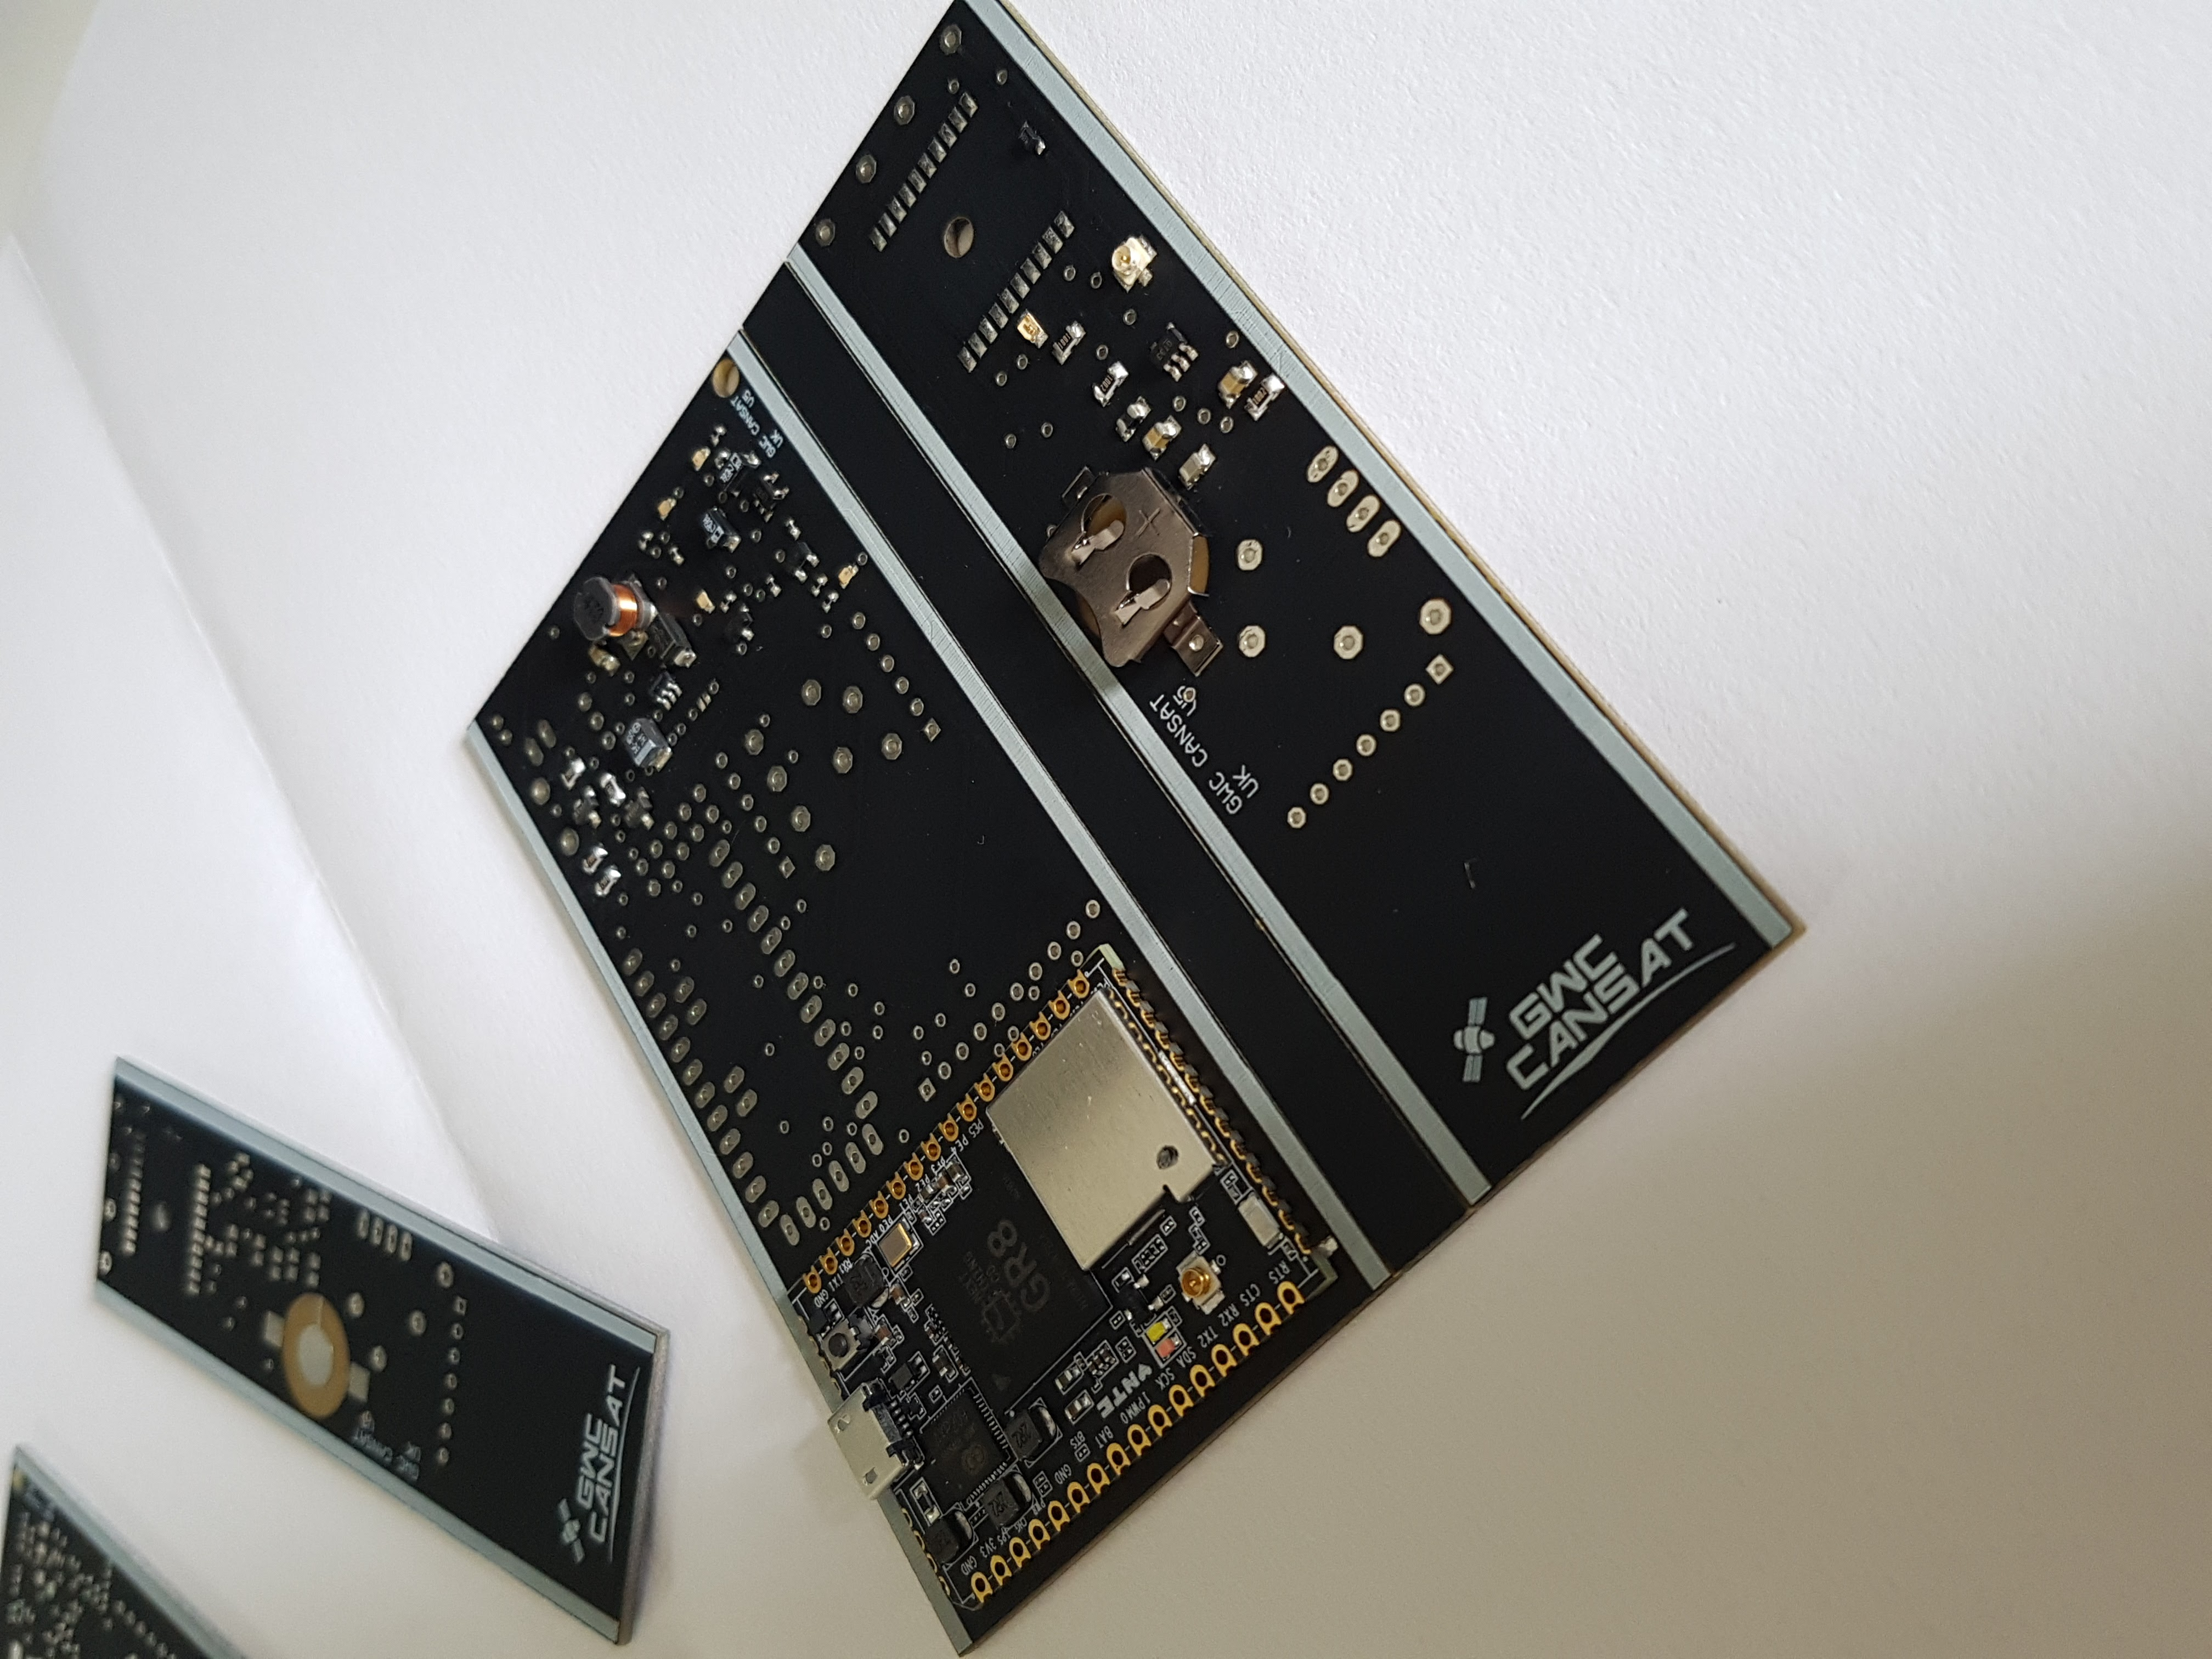
\includegraphics[scale=0.05, angle=270]{pcbs.jpg}\hspace*{\fill}
	\caption{Partially assembled CanSat PCBs}
	\label{pboardnew}
\end{figure}

With our new internal frame design the team was able to expand to two PCBs: a primary PCB with control, radio, and some sensor circuitry, and a secondary PCB with a larger array of sensors. We also included redundant level shifting and step-down voltage converters to ensure a reliable system.

As with our mechanical design, the team's electrical schematics and layouts are available at the team GitHub \footnote{https://github.com/Arcturus314/cansat2017\_design}, though a condensed schematic is shown in figure \ref{cschem}.

\begin{figure}[h]
	\hfill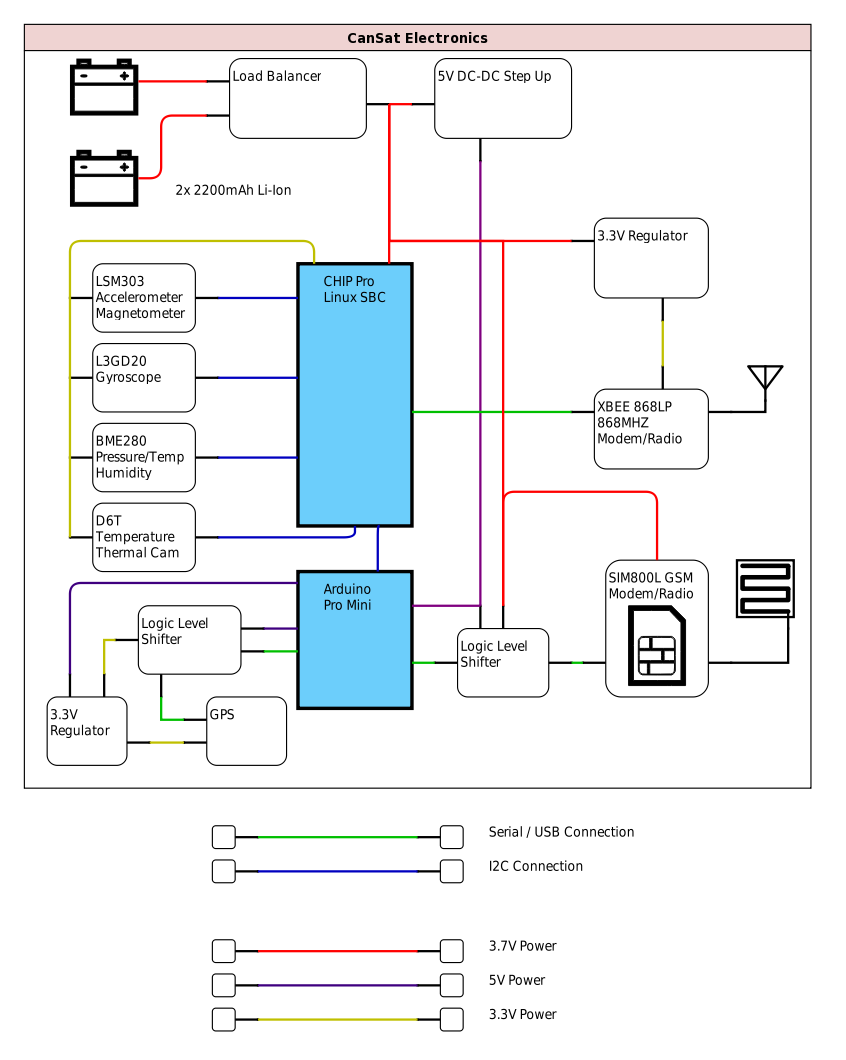
\includegraphics[scale=0.7]{CanSat-detail.png}\hspace*{\fill}
	\caption{A condensed schematic of the final CanSat}
	\label{cschem}
\end{figure}

\subsection{Radio Specifications}
\subsubsection{Prototype Design}
Our prototype design included two radios: an XBEE Pro 2.4GHz and a SIM800L GSM module. This dual radio design, as seen in the schematic in figure \ref{cschem}, provides redundancy and assists emergency recovery of the CanSat. If the primary radio link is lost, or CHIP failure is experienced, the CanSat GPS coordinates will be sent via SMS to a team member's cell phone. 

The XBEE Pro is a simple all-in-one radio and modem module allowing for long range encrypted communication over the 802.15.4 Zigbee protocol. At peak bandwidth, the modules are capable of a 250kbps transmit rate in either point to point or multi-point networks. The XBEE Pro consumes 215mA during data transmit and has a maximum range of 1.5km.

The team decided to use the XBEE module due to these features. The Zigbee protocol is widely used, making our CanSat compatible with thousands of data logging devices already in use, and the module's integrated spread-spectrum technology allows for reliable long-range communication in heavy interference. Finally, the modules can allow a transparent serial link between the CanSat and base station: the base station can access the CHIP Linux terminal with packetization handled onboard the XBEE. 

The SIM800L was chosen due to its cost, ubiquity, and large feature set. At USD 6.99 per unit including a breakout board, the module was easy to fit in our CanSat budget. Additionally, the SIM800L provides easy configuration via the well-documented AT command set. The SIM800L consumes approximately 40mA in receive mode, with millisecond spikes of up to 2A while transmitting.
\subsubsection{Final Design}
The team decided to continue using the SIM800L in the final CanSat design due to its ease of use. However, the move to custom PCBs allowed the team to utilize the XBEE 868LP: the only other long range XBEE module permitted for use in the European Union, which operates as a spread-spectrum device at 863-870MHz. The XBEE 868LP has the added benefits of lower power consumption at 48mA and a longer maximum range of 8.4km. These characteristics lead to a smaller transmit rate of 10kbps. However, the team accepted this loss due to the smaller packets resulting from rewritten CanSat code.
\subsection{Battery Specifications}
Our battery choice has remained constant through our prototype and final designs, with a pair of 2200mAh lithium ion cells connected via a load balancer.

There are many downsides associated with the use of lithium-ion cells. Their high energy density can lead to thermal runaway and combustion, damaging the CanSat, and battery performance suffers in cold temperatures. However, it is important to note that the CanSat will be dropped from a height of 1km: too low to see any major temperature delta. Additionally, our prototype CanSat has shown that the outer shell and internal frame provide enough support to protect the batteries. The team has also decided to include foam padding at the bottom of the battery compartment to further prevent damage.

CanSat power usage and estimated runtime:

	\begin{center}
	\begin{tabular}{ll}
		Sensor&Power Consumption\\
		\hline
		GPS&20mA \\
		MEMS sensors&10mA total \\
		CHIP Pro&270mA mean \\
		Arduino Pro Mini&15mA \\
		SIM800L&40mA \\
		XBEE 868LP&48mA \\
		Power Supply inefficiency&50mA approx\\
		\hline
		Total&413mA
	\end{tabular}	
	\end{center}	

With a 4400mAh battery, this leads to a calculated runtime of $\frac{4400}{413}=10.65$ hours. However, this calculation assumes that the CanSat is constantly transmitting: in real-world tests, the CanSat does not constantly transmit and hence reaches runtimes of between 12 and 13 hours.

\section{Software Design}
As both design revisions of the CanSat incorporated similar software only the final version will be described here.
\subsection{On-CanSat}
The CanSat software is divided between the main control, data logging, and processing loops running on the Linux SBC, and the control and interpretation loop running on the Arduino Pro Mini. All of our CanSat code is available in our team's software GitHub repository \footnote{https://github.com/Arcturus314/cansat2017}.
\subsubsection{Linux Single-Board-Computer}
The overall program structure is illustrated in figure \ref{pstruct}, though it is detailed further below.

%\begin{figure}[h]
%	\hfill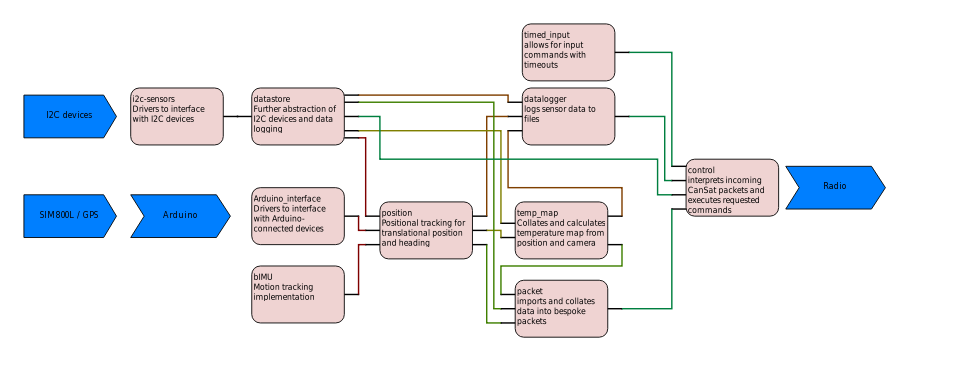
\includegraphics[scale=0.7, angle=90]{CanSat-software-diagram.png}\hspace*{\fill}
%	\caption{The on-CanSat program structure}
%	\label{pstruct}
%\end{figure}

\begin{sidewaysfigure}
	\centering
		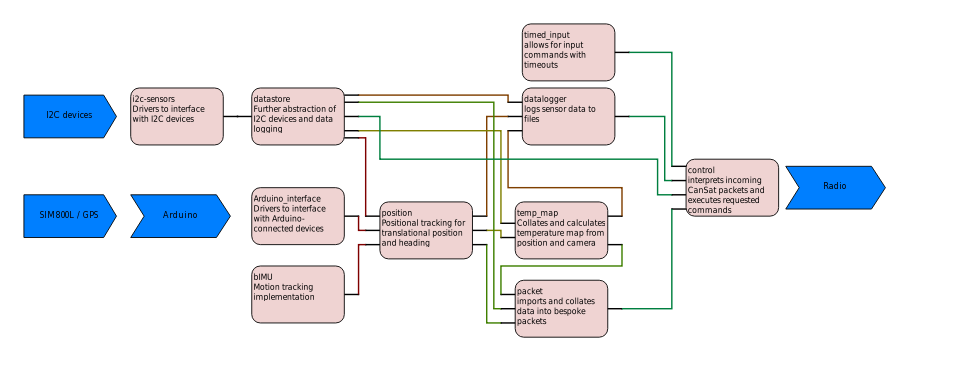
\includegraphics[scale=0.7]{CanSat-software-diagram.png}
	\caption{The on-CanSat program structure}
	\label{pstruct}
\end{sidewaysfigure}

All code used in the Linux system of the CanSat was written in Python, with a heavily customized version of Vim as a development environment. The program runs several tasks in parallel: packetization for radio transmission, data logging and backup, sensor and device control, and large-scale data processing for motion tracking and heat map creation.

The base level of the program occurs inside the i2c-sensors and arduino\_interface modules. These modules abstract the raw bus interfaces for the sensors and devices present on the CanSat, enabling simple read functions and easy set functions for sensor power, update rate, and full-scale deflection. The datastore module is built on i2c-sensors and further abstracts the CanSat sensor payload into a variety of different modes. So far, the team has implemented:

\begin{enumerate}
	\item min\_power: all sensors and devices aside from the Arduino, CHIP, and radio are disabled
	\item all\_active: all sensors and devices are active at full power, update, and deflection
	\item envir\_log: only sensors related to environmental data logging (humidity, temperature, and pressure) are active
	\item track\_pos: only sensors required for positional tracking (accelerometer, magnetometer, gyroscope, barometer, and GPS) are active
	\item heat\_map: only sensors required for heat map creation (accelerometer, magnetometer, gyroscope, barometer, GPS, and thermal camera) are active
\end{enumerate}

These sensor modes provide easy CanSat control, maximizing performance and battery life. The datastore module contains a variety of other features, including the ability to check sensor failure or i2c communication failure via the use of error catching code, and an implementation of functions abstracting calibration routines present in i2c-sensors.

The data collected from datastore and from arduino\_interface is also used to calculate CanSat position. This is done via a Kalman filter \footnote{http://www.olliw.eu/2013/imu-data-fusing/}, which calculates accurate pitch and roll from the accelerometer and gyroscope. The accuracy of this data is further improved via a tilt-compensated magnetometer. Via these filters, the CanSat is able to accurately track its 3D orientation.
However, translational positional tracking via accelerometer integration is prone to drift, and hence bounding sensors are necessary. This is accomplished via the barometer, from which altitude can be calculated, and the GPS, from which x-y position can be calculated to a precision of $\pm$5m.

Once position and heading can be accurately calculated, the CanSat then is able to map data collected from each pixel of the thermal camera to various regions on the ground. This can be done via simple trigonometry and rotation matrices. However, in order to ensure fast update rates, pixels are assumed to represent square regions of a flat ground surface, scaled by the CanSat displacement above the ground. These algorithms are accessible in the CanSat codebase and run in a distinct thread from data logging and radio communication. 

With data collected and processed from CanSat sensors, it is prepared for transmission via the packet module. The packet module, after receiving a data request from the control module, collects all required sensor data and assembles them into a packet. The contents of a packet can be arbitrarily requested and can include current sensor data points, stored sensor data points, sensor error data, positional data, and temperature maps. It is also possible to request pre-made packets with data from the modes described in datastore. Packets are also appended with a checksum, which allows the base station to confirm packet validity. Packet structure is detailed in the packet module in the CanSat codebase. 

Overall CanSat control is done via the control module, which serves to interpret base station packets, change all necessary sensor settings, and instantiate a module to log data to a text file. The control module also allows for text messaging if many malformed packets are received.

The Linux subsystem of the CanSat receives approximately 26kbps of data. However, much of this data is due to the high update rate for inertial sensors required for accurate positional tracking and is therefore not sent to the base station. Packets are also not sent at regular intervals: the dynamic nature of the CanSat packetization and control algorithms has led to a tested update rate of 2-5Hz over a radio link.

\subsubsection{Arduino}
Written in C++ in the Arduino IDE, the Arduino codebase is relatively simple. Via Adafruit libraries \footnote{https://learn.adafruit.com/adafruit-ultimate-gps/arduino-wiring} GPS position, speed, altitude, and validity is read from the GPS module and split into character lists, which are then transmitted to the Linux subsystem. The Arduino codebase also allows for SIM800L text messaging integration.

\subsection{Base Station}
The base station codebase allows easy visualization of CanSat data and overall control of the CanSat. It uses two discrete loops, one requesting data from the CanSat and the other graphing said data in a graphical user interface and providing CanSat status information. Via a set of buttons, the base station allows for sensor, power mode, and deflection settings to be constructed in packets and sent to the CanSat. The base station also performs independent data logging of received data. The base station in test mode is visible in figure \ref{bstation}, and program flow can be seen in figure \ref{bflow}.

The base station code is written in Java / JavaFX within the Eclipse IDE.

\begin{sidewaysfigure}
	\hfill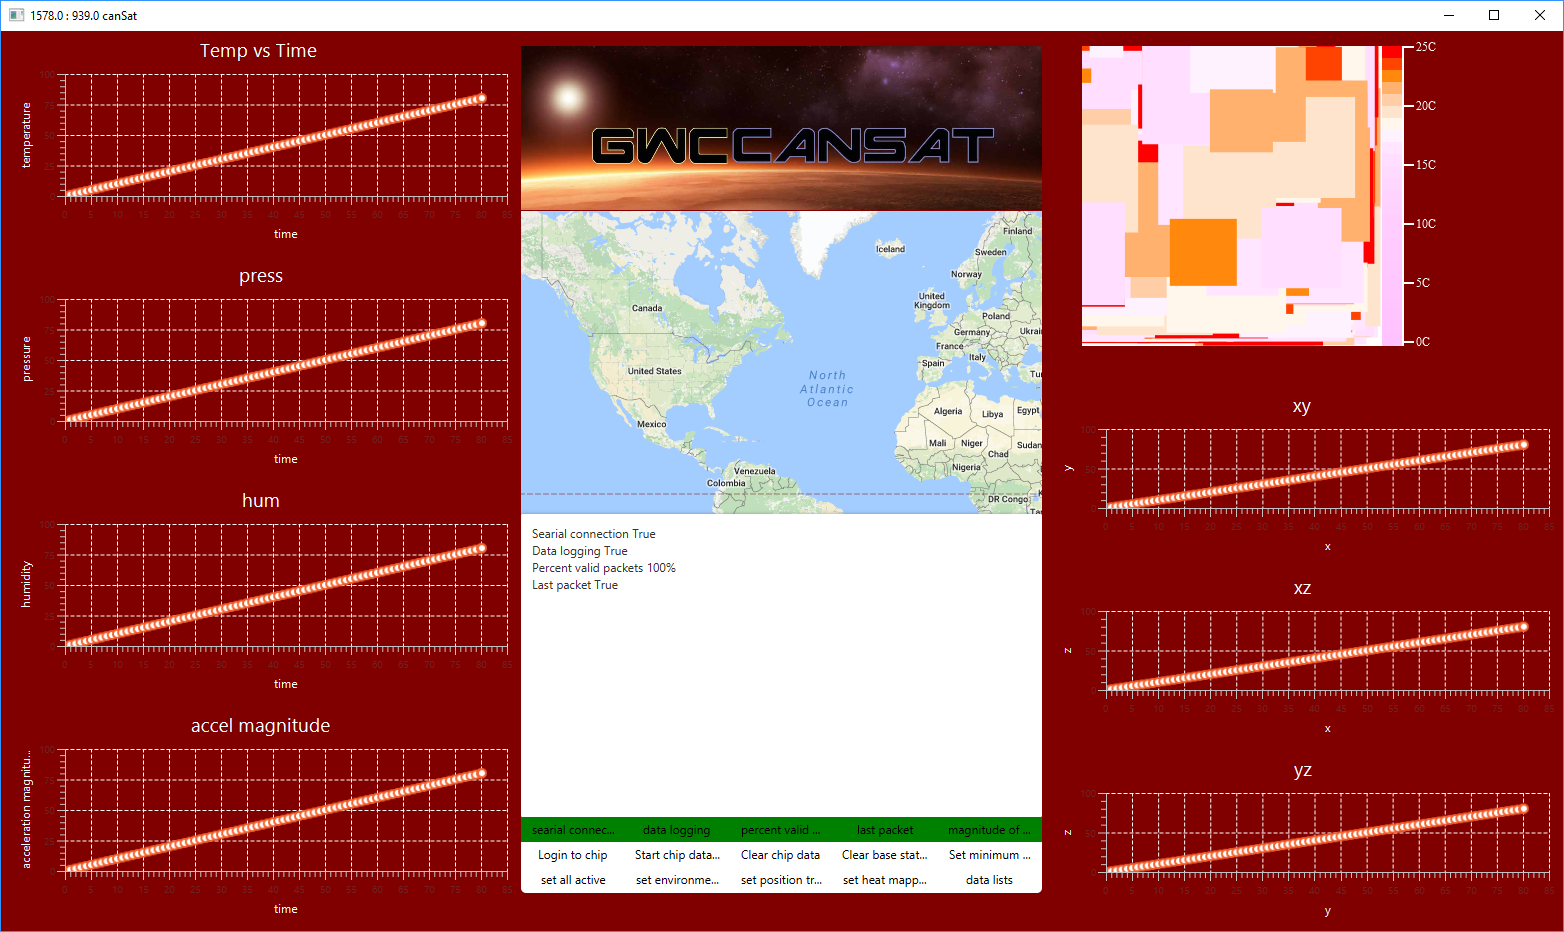
\includegraphics[scale=0.55]{base_station.png}\hspace*{\fill}
	\caption{The base station program running in test mode}
	\label{bstation}
\end{sidewaysfigure}

\begin{figure}[h]
	\hfill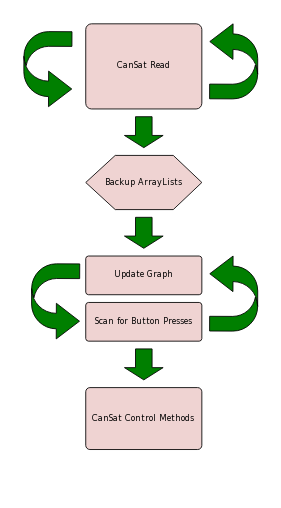
\includegraphics[scale=0.7]{Base-Station-program-flow.png}\hspace*{\fill}
	\caption{Overall flow for the base station program}
	\label{bflow}
\end{figure}

\section{Recovery System}
The team is currently using a simple hexagonal parachute made from ripstop nylon, which has led to a tested descent rate of approximately 10.5ms-1. The parachute is attached via a set of strings that loop within the upper internal frame, as can be seen in figure \ref{pmounts}.
With an estimated 1000m drop, this design will lead to a flight time of approximately 95 seconds. However, the team is working on implementing a more advanced, custom parachute with a cruciform design to improve CanSat stability during flight.

\begin{figure}
	\centering
	\begin{subfigure}{.5\textwidth}
		\centering
		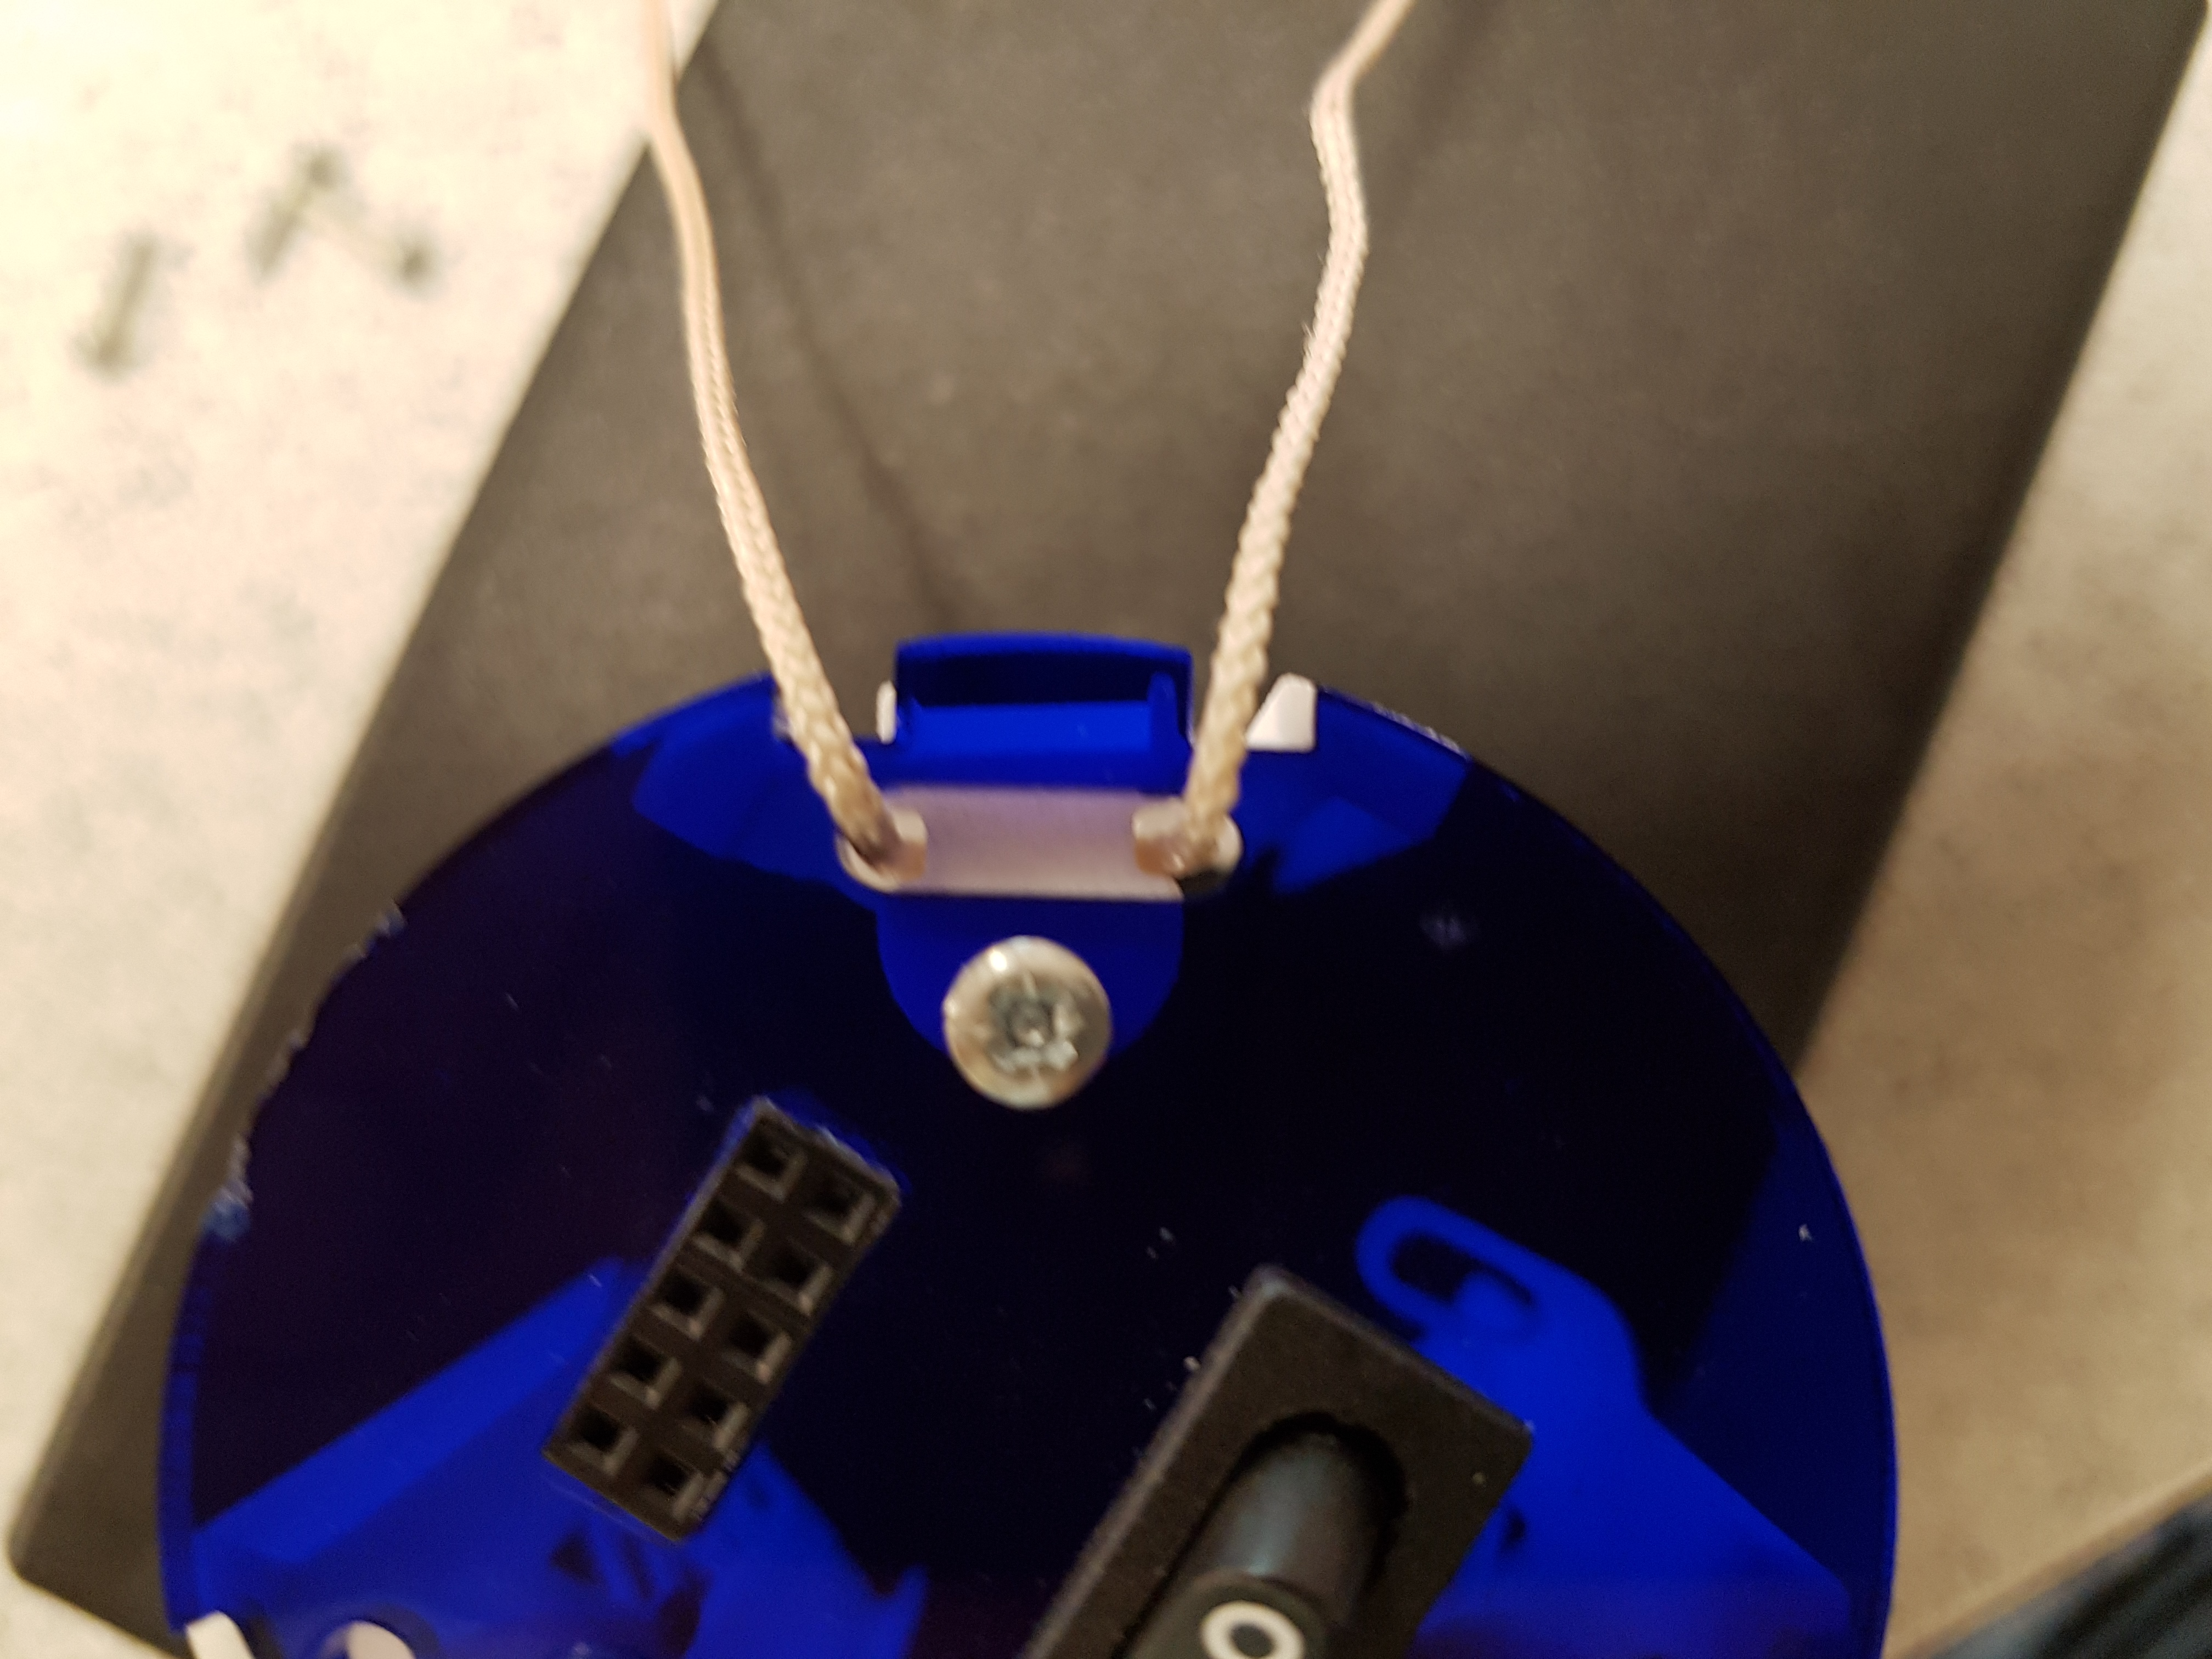
\includegraphics[width=.9\linewidth]{pmount.jpg}
	\end{subfigure}%
	\begin{subfigure}{.5\textwidth}
		\centering
		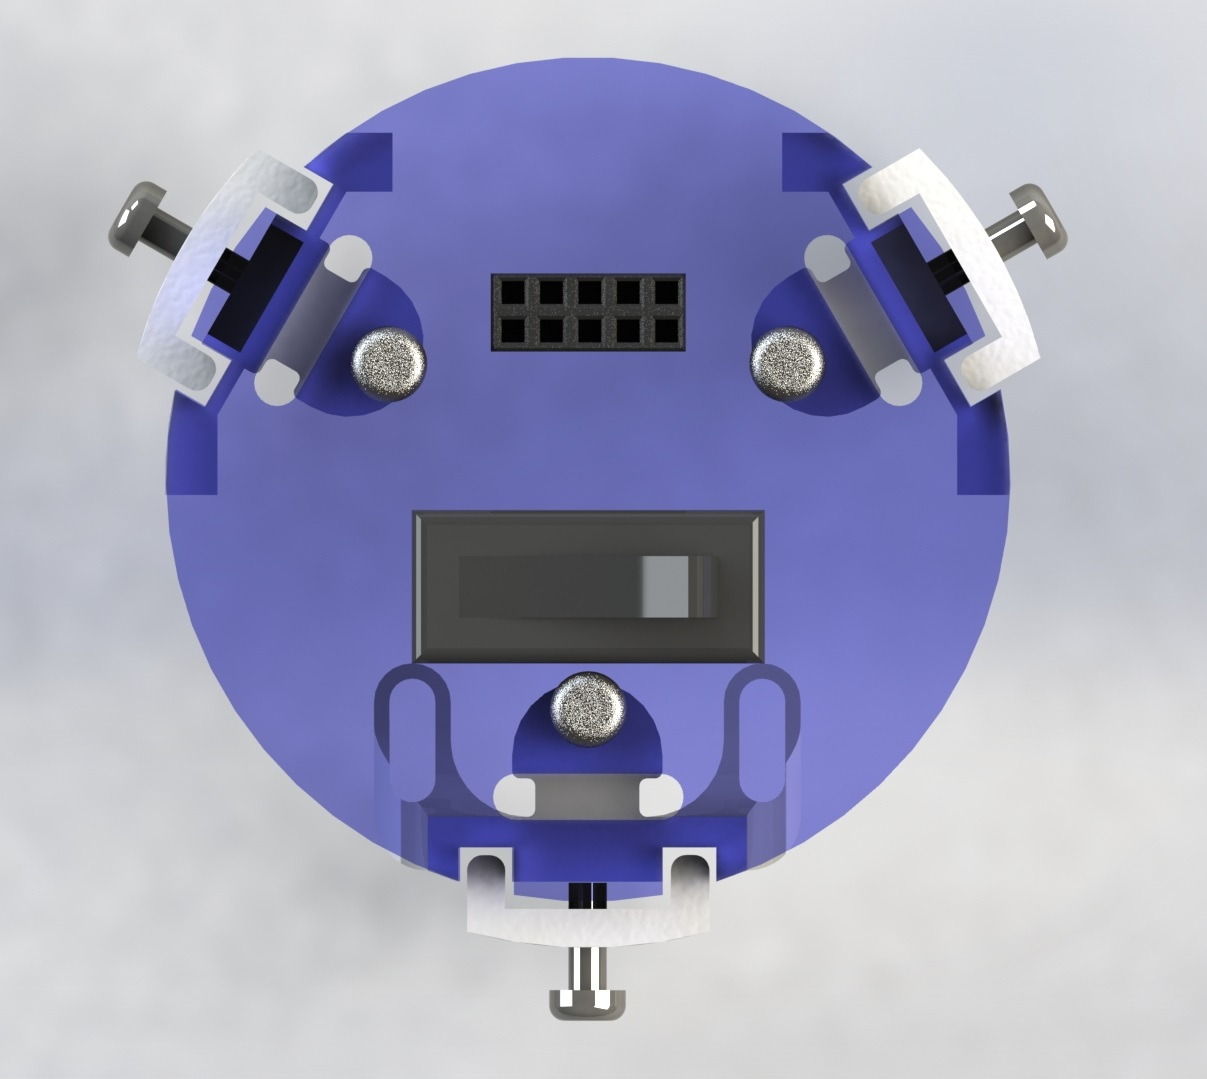
\includegraphics[width=0.8\linewidth, angle=0]{Parachute_mounts.jpg}
	\end{subfigure}
	\caption{Parachute mounts on the CanSat}
	\label{pmounts}
\end{figure}

\section{Ground Support Equipment}
Our base station design is relatively simple, containing only an XBEE 868LP module, an acrylic box with a development board serving as an XBEE mount and USB-Serial converter, as well as an 11dBm Yagi-Uda antenna. The USB-Serial converter is attached to a laptop running the base station software. The assembled base station can be seen in figure \ref{bsradio}.

\begin{figure}[h]
	\hfill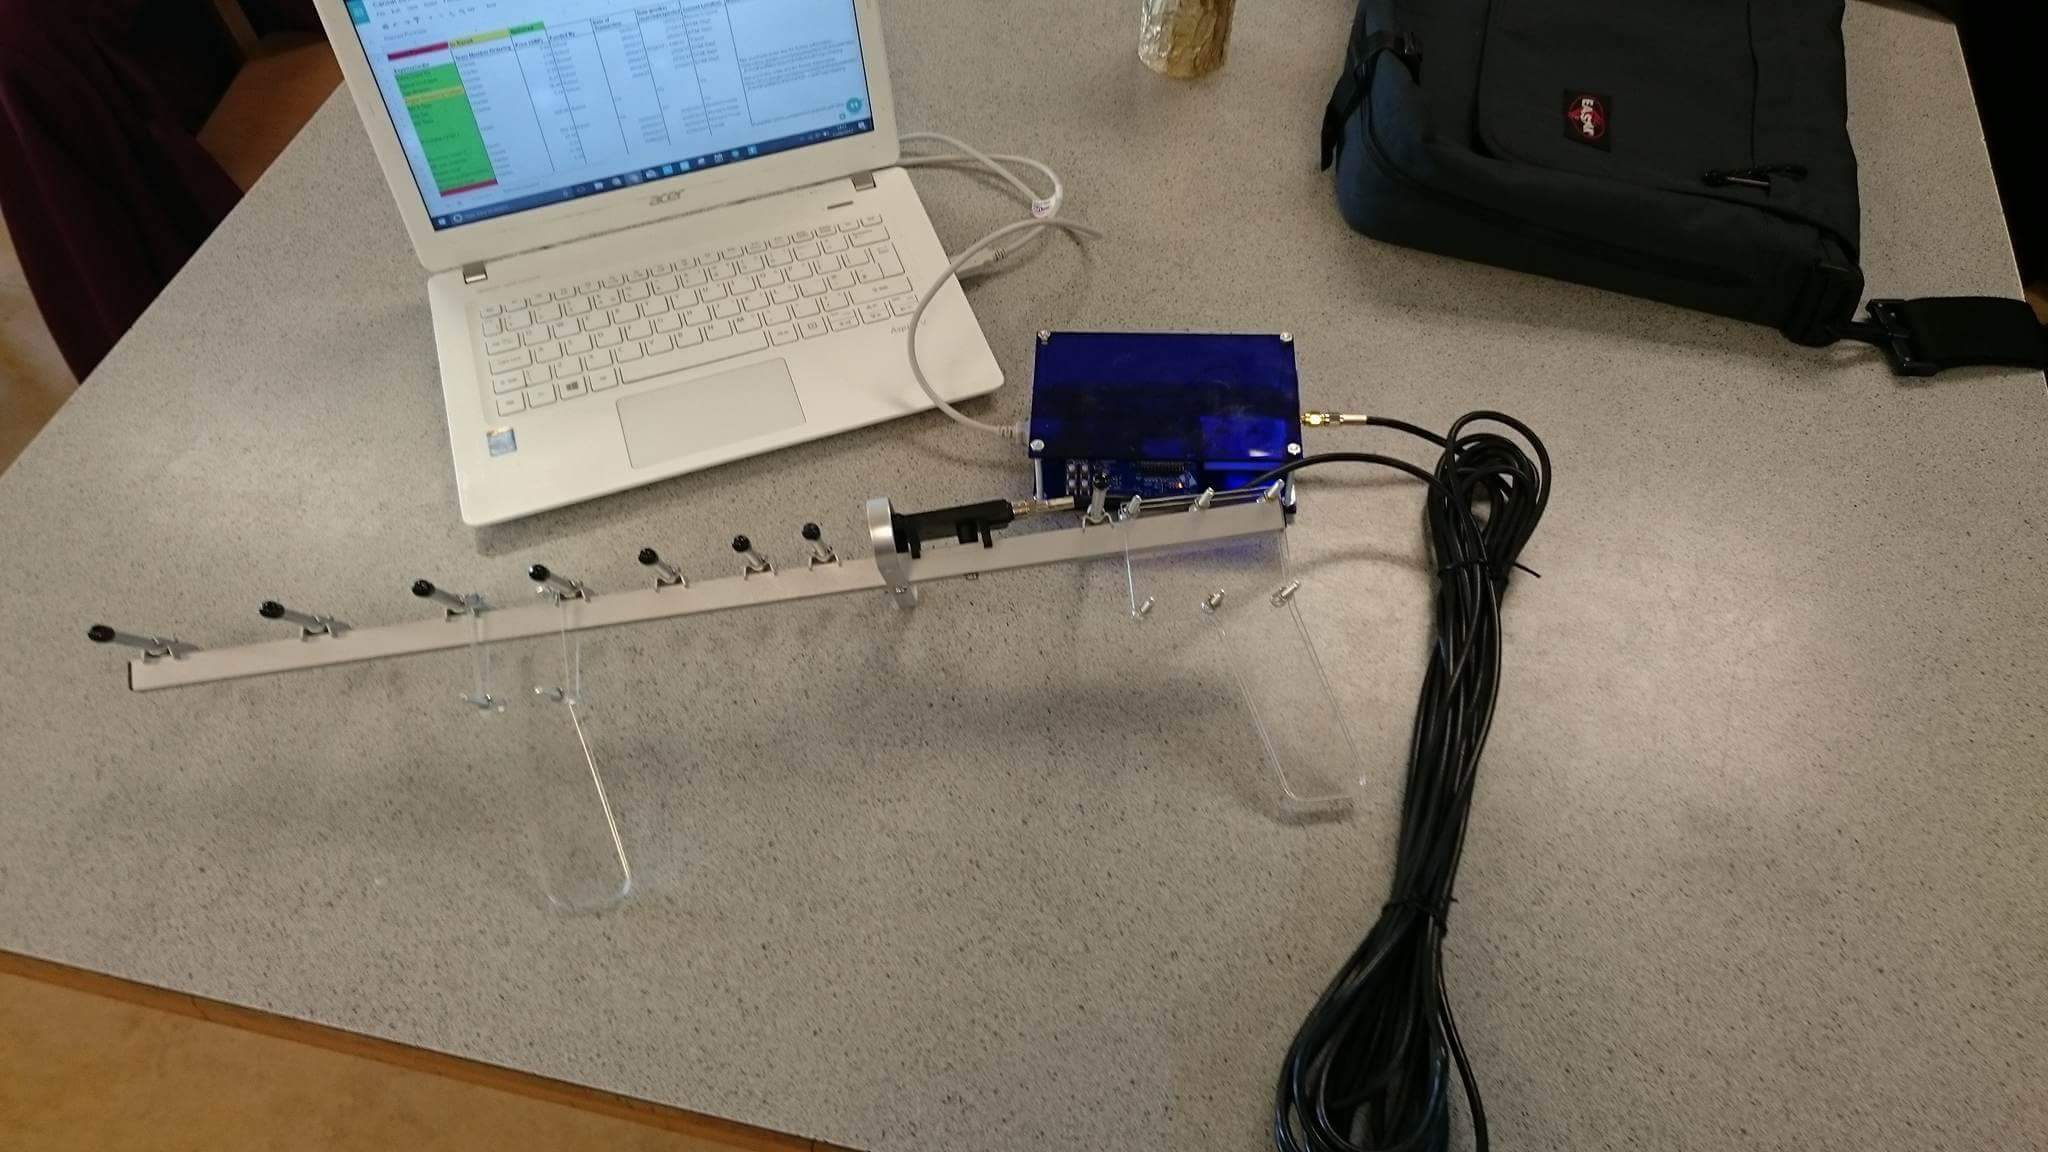
\includegraphics[scale=0.2]{bsradio.jpeg}\hspace*{\fill}
	\caption{The assembled base station}
	\label{bsradio}
\end{figure}

\chapter{Project Planning}
\section{Design Schedule}
Throughout the season, our project planning was done through the applications Trello, Meekan, and Slack. However, these do not transfer well to a print medium such as this report, and hence the most important deadlines have been rewritten in table form.

\begin{center}
	\begin{longtable}{ll}
		\textbf{Task}	                                                                        & \textbf{Deadline}   \\  \hline
		1 Mechanics                                                                 &            \\ \hline
		1.1 Create prototype fiberglass shell                                       & 10/16/2016 \\
		1.2 Run durability tests on fiberglass shell                                & 10/20/2016 \\
		1.3 Create final fiberglass shell                                           & 5/15/2017  \\
		1.4 Machine final fiberglass shell                                          & 5/18/2017  \\
		1.5 Create CAD models of sensors, development boards, and radios            & 5/1/2017   \\
		1.6 Brainstorm internal CanSat layout                                       & 3/1/2017   \\
		1.7 Create CAD model of internal CanSat layout                              & 4/1/2017   \\
		1.8 Create CAD model of internal frame and sliders                          & 4/1/2017   \\
		1.9 Brainstorm manufacturing options for internal frame                     & 4/5/2017   \\
		1.10 Manufacture internal supports / frame from CAD                         & 5/1/2017   \\
		1.11 Assemble mechanical portion of CanSat                                  & 6/1/2017   \\ \hline
		2 Electronics                                                               &            \\ \hline
		2.1 Decide on final capability list                                         & 10/1/2016  \\
		2.2 Select sensors, MCU, and radio to fulfill final capability list         & 11/1/2016  \\
		2.3 Select required battery size and technology to support sensors and MCU  & 11/6/2016  \\
		2.4 Order sensors, MCU, radio, and battery                                  & 11/10/2016 \\
		2.5 Test system on a breadboard                                             & 12/1/2016  \\
		2.6 Design PCB layouts for internal electronics                             & 5/1/2016   \\
		2.7 Order PCBs                                                              & 5/3/2016   \\
		2.8 Assemble electronics portion of CanSat                                  & 6/1/2016   \\
		2.9 Conduct radio tests with MCU and PC                                     & 6/10/2016  \\
		2.10 Test radio range between MCU and PC                                    & 6/10/2016  \\ \hline
		3 Software                                                                  &            \\ \hline
		3.1 Create basic “hello world” program for MCU                              & 12/1/2016  \\
		3.2 Create basic sensor tests for MCU                                       & 12/15/2016 \\
		3.3 Create graphing and IO system for PC                                    & 2/1/2017   \\
		3.4 Implement two way communication capability between PC and CanSat        & 3/1/2017   \\
		3.5 Create unified data logging and and telemetry system and API for CanSat & 5/1/2017   \\
		3.6 Create final PC program incorporating all tested features               & 6/1/2017   \\ \hline
		4 Recovery System                                                                 &            \\ \hline
		4.1 Brainstorm and prototype initial parachute designs                      & 11/1/2016  \\
		4.2 Test prototype parachute designs                                        & 12/1/2016  \\
		4.3 Create and test final parachute                                         & 1/1/2016   \\ \hline
		Advertisement and Sponsorship                                               &            \\ \hline
		5.1 Discuss sponsorship options with school                                 & 10/1/2016  \\
		5.2 Discuss sponsorship options with interested companies                   & 12/1/2016  \\
		5.3 Acquire 2000 GBP total in funding                                       & 3/1/2016   \\
		5.4 Create advertising materials for school Open Day                        & 11/23/2016 \\
		5.5 Create presentation for school assembly                                 & 3/18/2017  \\
		5.6 Decide on activities for P5 workshop                                    & 4/9/2017   \\
		5.7 Collect materials and design experiment for P5 workshop                 & 4/18/2017  \\
		5.8 Participate in Edinburgh Maker Faire                                    & 4/16/2017  \\
		5.9 Create materials for Edinburgh Maker Faire                              & 4/12/2017  \\
		5.10 Set up social media accounts                                           & 10/1/2016  \\
		5.11 Create temporary website                                               & 10/1/2016  \\
		5.12 Create permanent website                                               & 1/1/2016   \\
		5.13 Migrate materials to permanent website                                 & 1/5/2016  
	\end{longtable}
\end{center}

\section{Resource Estimation}

Our CanSat budget is described below:
\begin{center}
\begin{longtable}{llll}
	Component Name              & Unit Price (USD) & Total Price (USD) & Price (EUR) \\ \hline
	XBEE 868LP For Europe       & n/a              & n/a               & 20.71       \\
	NTC CHIP Pro                & 16               & 16                & 14.4        \\
	Adafruit 9DOF IMU           & 19.99            & 19.99             & 17.991      \\
	Omron D6T                   & 42.9             & 42.9              & 38.61       \\
	Adafruit BME280             & 19.95            & 19.95             & 17.955      \\
	FGPMMOPA6H GPS              & 11.35            & 11.35             & 10.215      \\
	Antenna 868MHz              & 6.82             & 6.82              & 6.138       \\
	Thermal Sensor Contact      & 0.0784           & 0.3136            & 0.28224     \\
	Thermal Sensor Housing      & 0.125            & 0.125             & 0.1125      \\
	Female 5x2 Header           & 0.85             & 0.85              & 0.765       \\
	Parachute                   & 7.37             & 7.37              & 6.633       \\
	4400mAh Li-Ion battery      & 19.95            & 19.95             & 17.955      \\
	Wire (assorted)             & 5                & 5                 & 4.5         \\
	PCB (primary and secondary) & 59.12            & 59.12             & 53.208      \\
	GSM Module                  & 6.18             & 6.18              & 5.562       \\
	Plastic Frame               & 67.55            & 67.55             & 60.795      \\
	Fibreglass                  & 10               & 10                & 9           \\
	Passive Components          & 18.98            & 18.98             & 17.082      \\
	RP-SMA U.FL adapter         & 11.98            & 11.98             & 10.782      \\
	Power Switch                & 0.94             & 0.94              & 0.846       \\ \hline
	Sum:                        &                  & 325.3686          & 313.54174   \\         
\end{longtable}
\end{center}

\section{External Support}

The team has received sponsorships from:
\begin{center}
\begin{tabular}{ll}
	Sponsor Name                 & Funding Given (GBP)                           \\ \hline
	George Watson's College      & 1000                                          \\
	Kaiam Corporation            & 600                                           \\
	Enviromentor                & 500                                           \\
	Holmes Hines Memorial Fund   & 500                                           \\ \hline
	Sponsor Name                 & Sponsorship Materials                         \\ \hline
	Sketchfab                    & Access to pro licenses for 3D export software \\
	Tecbridge Circuits           & Custom printed circuit boards                 \\
	Croft Additive Manufacturing & Custom 3D steel printing                      \\
	Next Thing Co                & CHIP Pro units                                \\
	Spirit Circuits              & Custom printed circuit boards                 \\
	London Manufacturing         & Subsidized PCB assembly                       \\
                                           
\end{tabular}
\end{center}

The team has also received support from George Watson's College via access to tools in their Technology department, Heriot Watt University for milling and bending aluminum, and from Tecbridge Circuits for PCB design assistance.

\section{Test Plan}
\subsection{Radio Testing}
We have tested our Yagi-Uda antenna and duck antenna with XBEE 868LP modules, simulating the base station and CanSat, in a nearby large field.  We obtained a range of 2.3km, although we had lost line of sight due to tree cover.

We have also tested the XBEE 868LP modules with 1$\lambda$ antennae, leading to a range of 2.5km under similar conditions.
\subsection{Outer Shell Testing}
Our outer shells have been tested and proven viable in the UK CanSat competition. Before the UK Competition, we had drop-tested weighted outer shells without parachutes from a height of 10m and filmed their impact in slow motion. This video confirmed the spring-like properties of the fiberglass that would provide protection to the CanSat.
\subsection{Parachute Testing}
Our parachutes have also been proven viable in the UK CanSat competition with a 10.5ms-1 descent rate. Before the competition, we tested descent rate with 300g masses and a parachute attachment mechanism used in the actual CanSat. The parachute deployed successfully in 28 / 30 tests: the two failures were due to the parachute only partially unfurling before collision with the ground- this won't pose a problem in the context of a 1km drop.
\subsection{Primary Mission Testing}
The translational position and orientation tracking have been confirmed working via in-house tests at low acceleration. We plan to test positional tracking in a drop-test scenario before the competition. 

We have also confirmed that the thermal camera mapping algorithm functions provided accurate data from the positional tracking algorithms.
\section{Outreach}
Our team has taken a multifaceted approach to CanSat outreach, presenting at school events, events open to the public, and via websites and social media.
\subsection{Online Presence}
Our team has social media available on many platforms, including Facebook\footnote{https://www.facebook.com/cansatgwc}, Instagram\footnote{https://www.instagram.com/cansatgwc/}, and Twitter\footnote{https://twitter.com/cansatgwc2016}. Frequent updates and usage of social media tags allow us to draw people interested in our team and in the competition to our pages. We have and have planned to continue frequently updating our social media pages, through the entirety of the team's journey through the UK and EU competitions.

The team has also designed a website to provide further online presence to our CanSat, to the CanSat competition, and to our sponsors. Our website is also frequently updated: a current snapshot can be seen in figure \ref{smedia}. 

\begin{figure}
	\centering
	\begin{subfigure}{.5\textwidth}
		\centering
		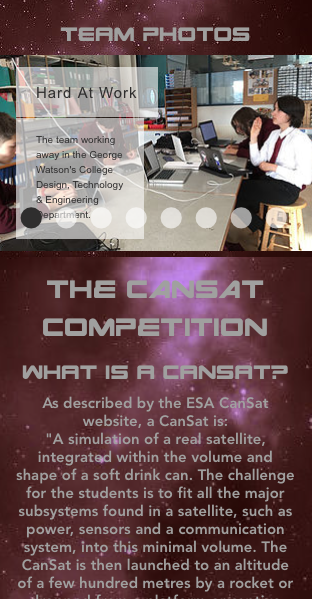
\includegraphics[width=.6\linewidth]{website.png}
	\end{subfigure}%
	\begin{subfigure}{.5\textwidth}
		\centering
		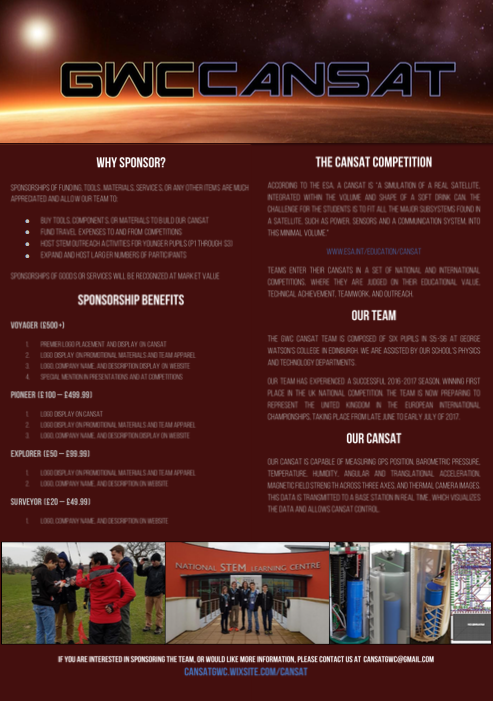
\includegraphics[width=0.8\linewidth, angle=0]{brochure.png}
	\end{subfigure}
	\caption{Various CanSat outreach materials}
	\label{smedia}
\end{figure}

The team has also created a sponsorship brochure for the upcoming season, which can be seen in figure \ref{smedia}.

Our CanSat and team have also received substantial press, including articles on and in 3dprint.com\footnote{https://3dprint.com/175578/esa-cansat-competition-3d-print/}, tctmagazine.com\footnote{http://www.tctmagazine.com/3D-printing-news/croft-additive-manufacturing-provide-slm-3d-printed-casting-/}, stem.org.uk\footnote{https://www.stem.org.uk/esero/students-soar-success-space-competition}, Edinburgh Evening News \footnote{March 20th 2017}, @STEMLearningUK Twitter\footnote{https://twitter.com/STEMLearningUK/status/842463014397829122}, gwc.org.uk\footnote{https://www.gwc.org.uk/news/satellite-simulation-win-takes-team-to-european-finals/}, and @GWC\_News Twitter\footnote{https://twitter.com/GWC\_News/status/841582764491190272}.
\subsection{In-Person Outreach}
The team has also performed several in-person outreach events. We have run presentations in technology and physics for school open days, and have run full-school presentations to expand on our team and on the competition. In one full school presentation, we presented our success at the UK competition in the context of the successes and failures we experienced as a team new to the CanSat competition, explaining the difficulties we've faced and the solutions we've implemented to solve these issues.

We have also initiated and ran educational outreach events for 9-10 year-old students. In the first session of the two-part workshop, students designed parachutes to meet certain descent velocity criteria: a reflection of the challenge we experienced in the UK CanSat competition. In the second section of the workshop, groups of students designed enclosure and padding to protect an egg dropped with their previously built parachute. To conclude the workshop, students tested their enclosure and parachute in a real-world egg drop. Some pictures of the event can be seen in figure \ref{eggdrop}.

\begin{figure}
	\centering
	\begin{subfigure}{.5\textwidth}
		\centering
		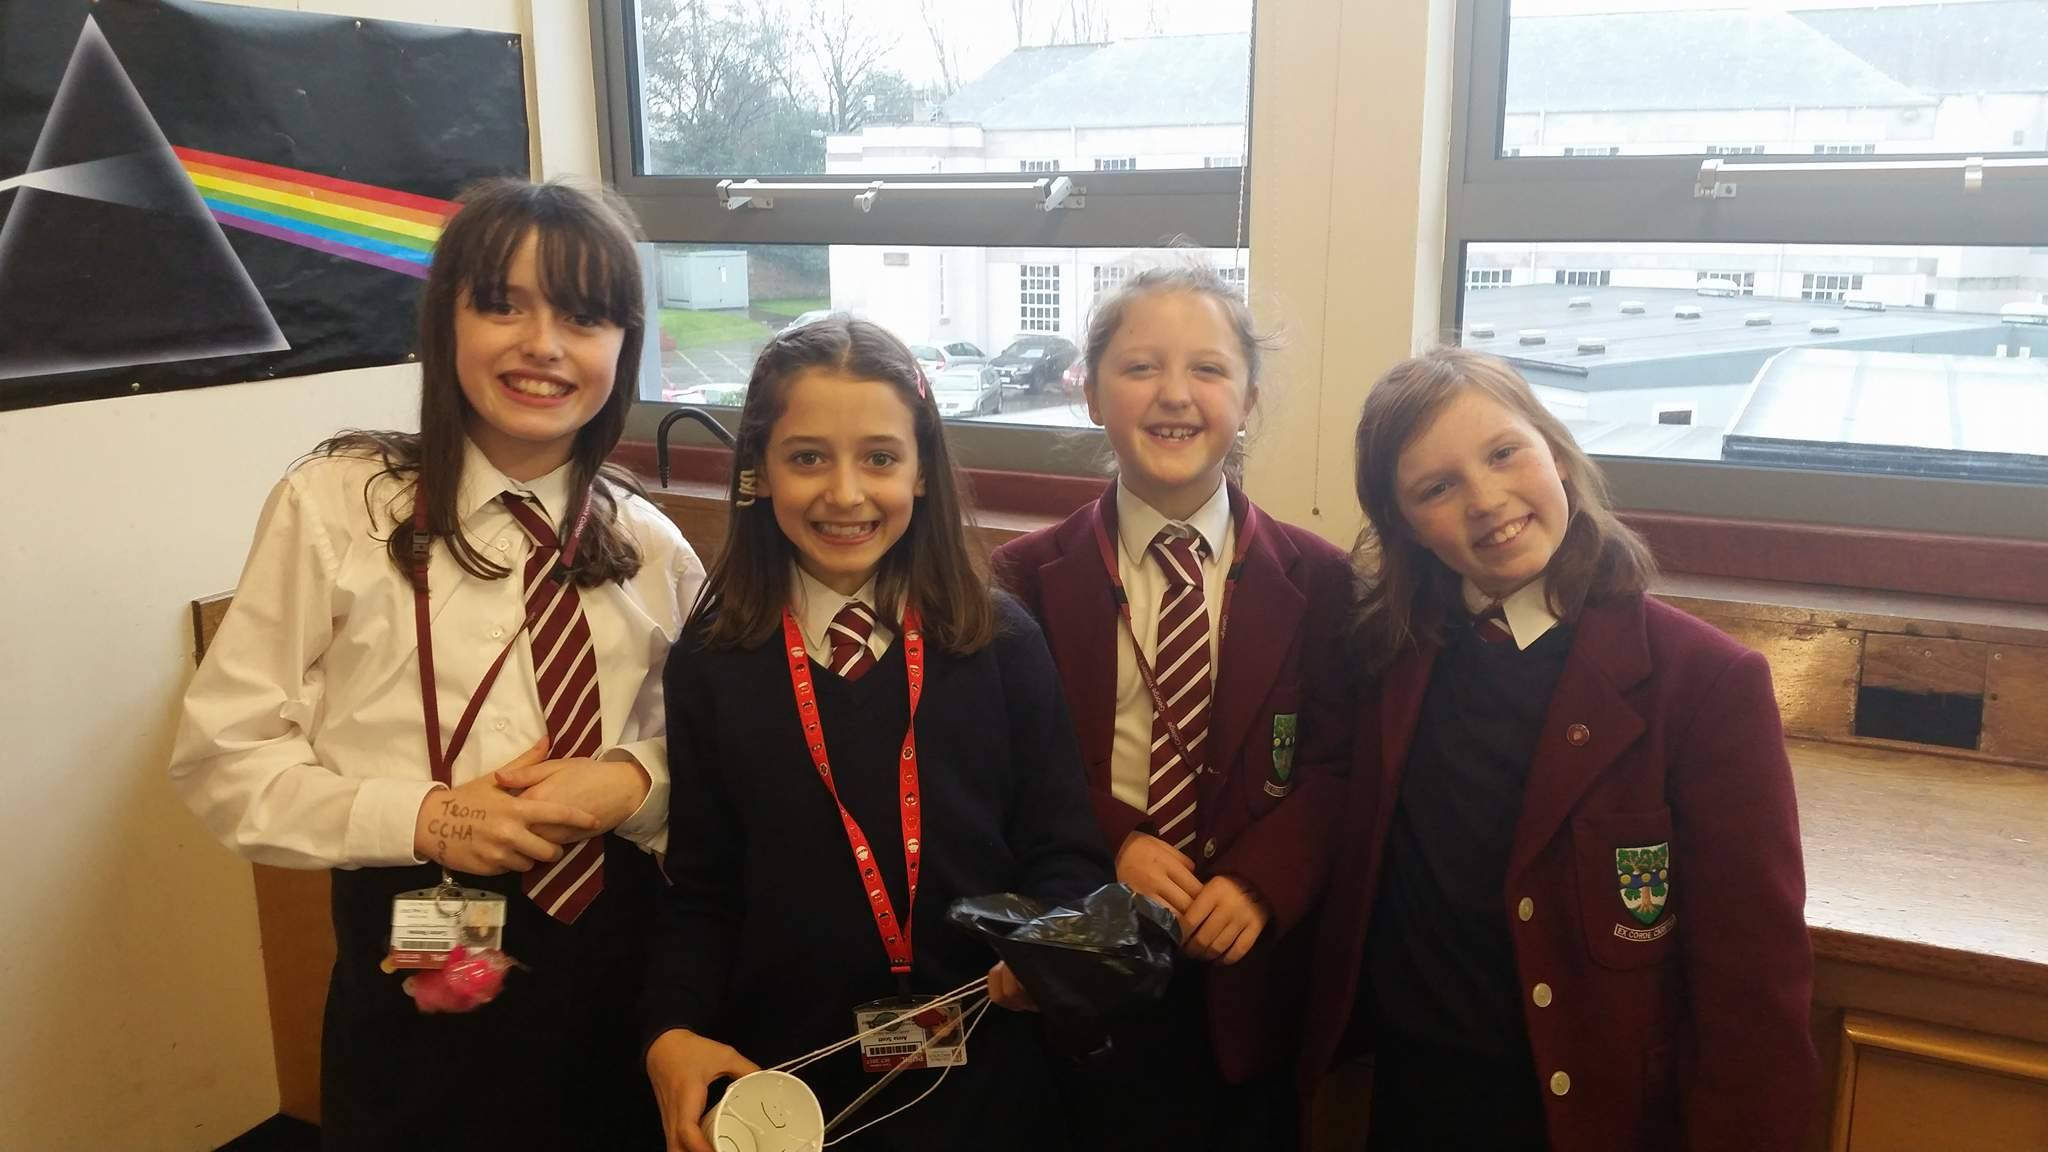
\includegraphics[width=.8\linewidth]{ed1.jpg}
	\end{subfigure}%
	\begin{subfigure}{.5\textwidth}
		\centering
		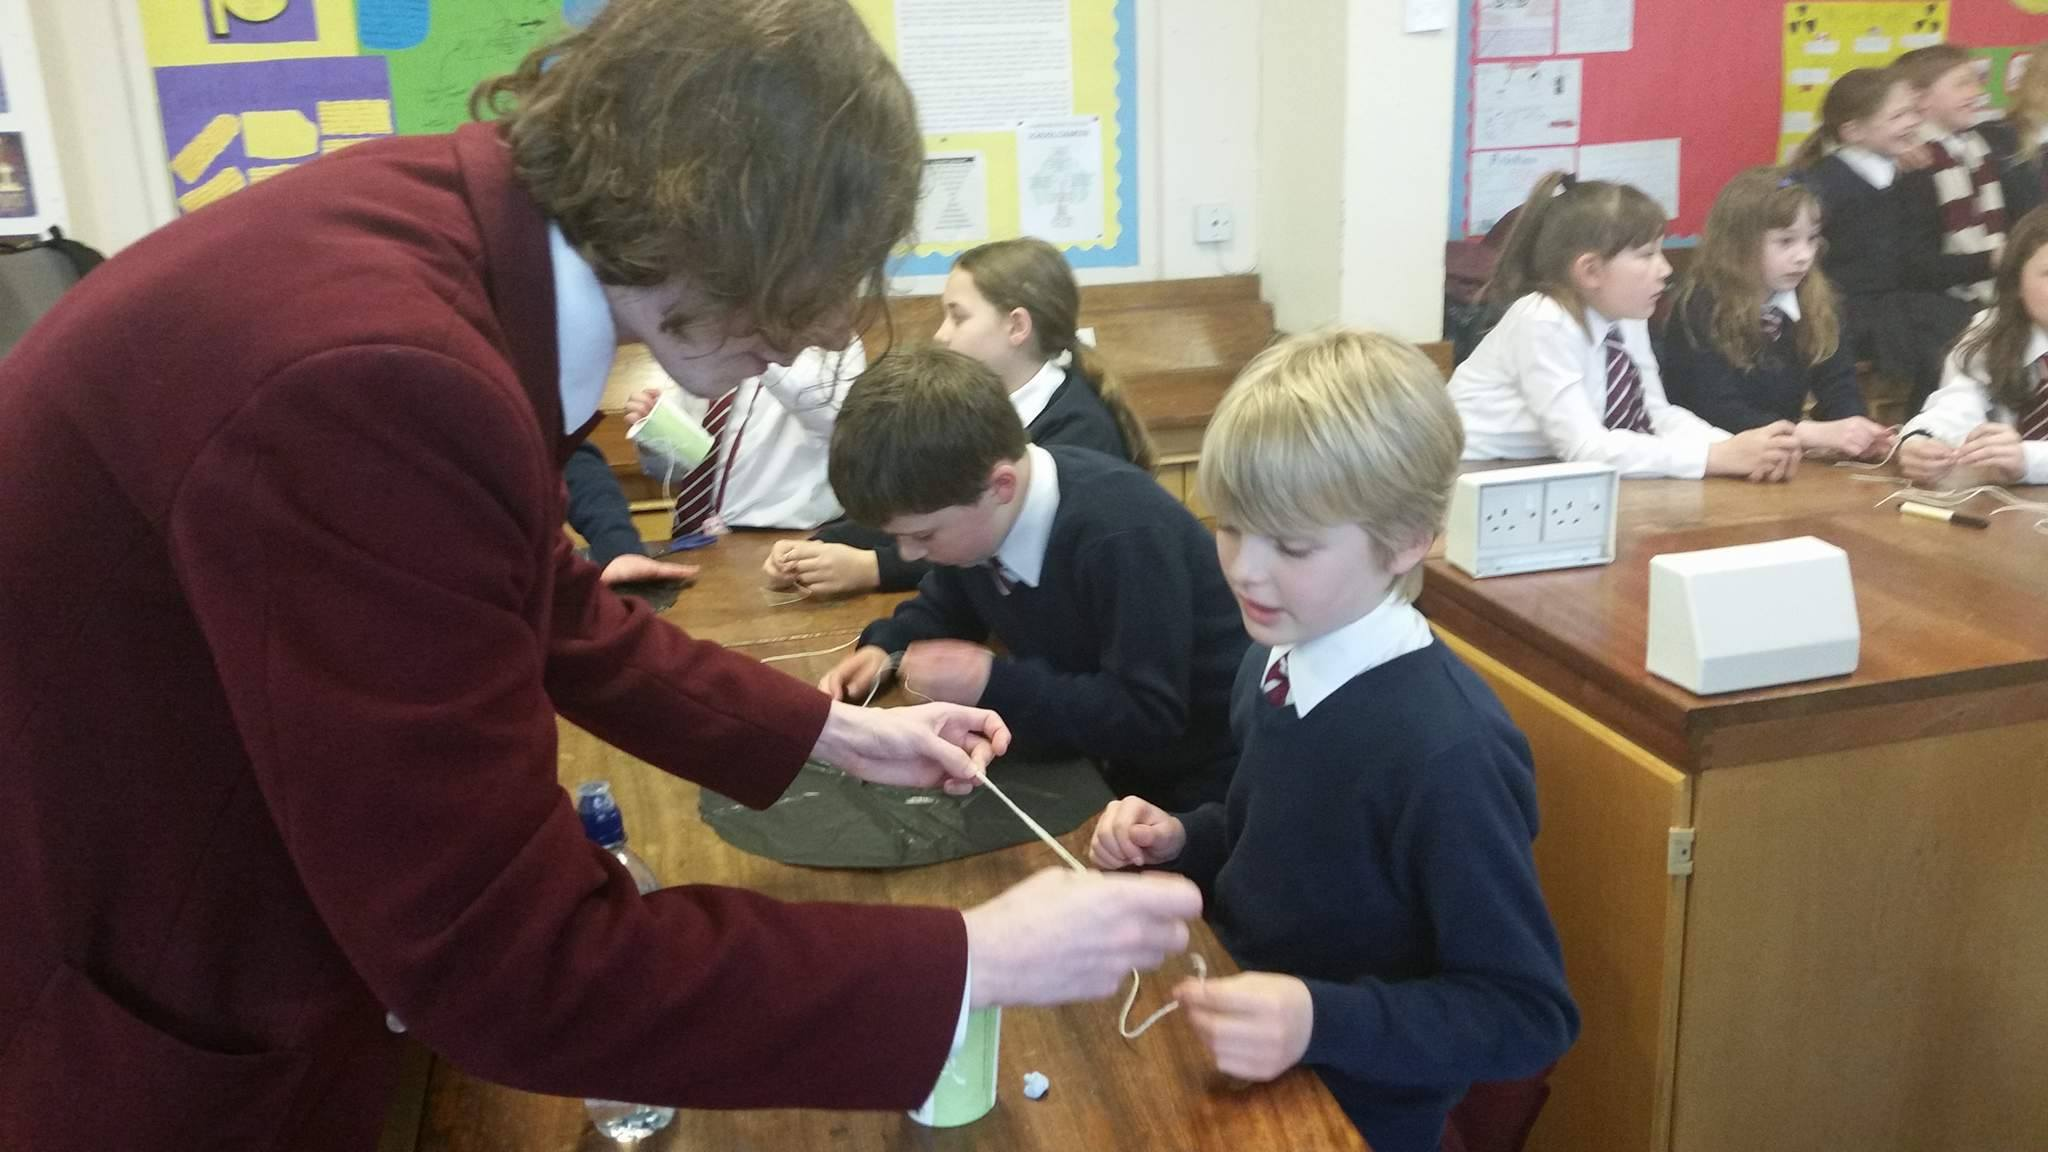
\includegraphics[width=0.8\linewidth, angle=0]{ed2.jpg}
	\end{subfigure}
	\caption{Participants in the egg drop workshop}
	\label{eggdrop}
\end{figure}

Finally, the team presented in the Edinburgh Mini Maker Fair during the Edinburgh Science Festival. This gave the team the opportunity to present our progress within the competition as well as speak to other people interested in what we have been doing. This included a slideshow of pictures of the CanSat and the team's trip to York for the UK National Competition as well having a demonstration of the working CanSat, plotting data on graphs on a display. The team was also open to questions from the general public during the entirety of the Maker Faire. Our booth can be seen in figure \ref{mfair}.

\begin{figure}[h]
	\hfill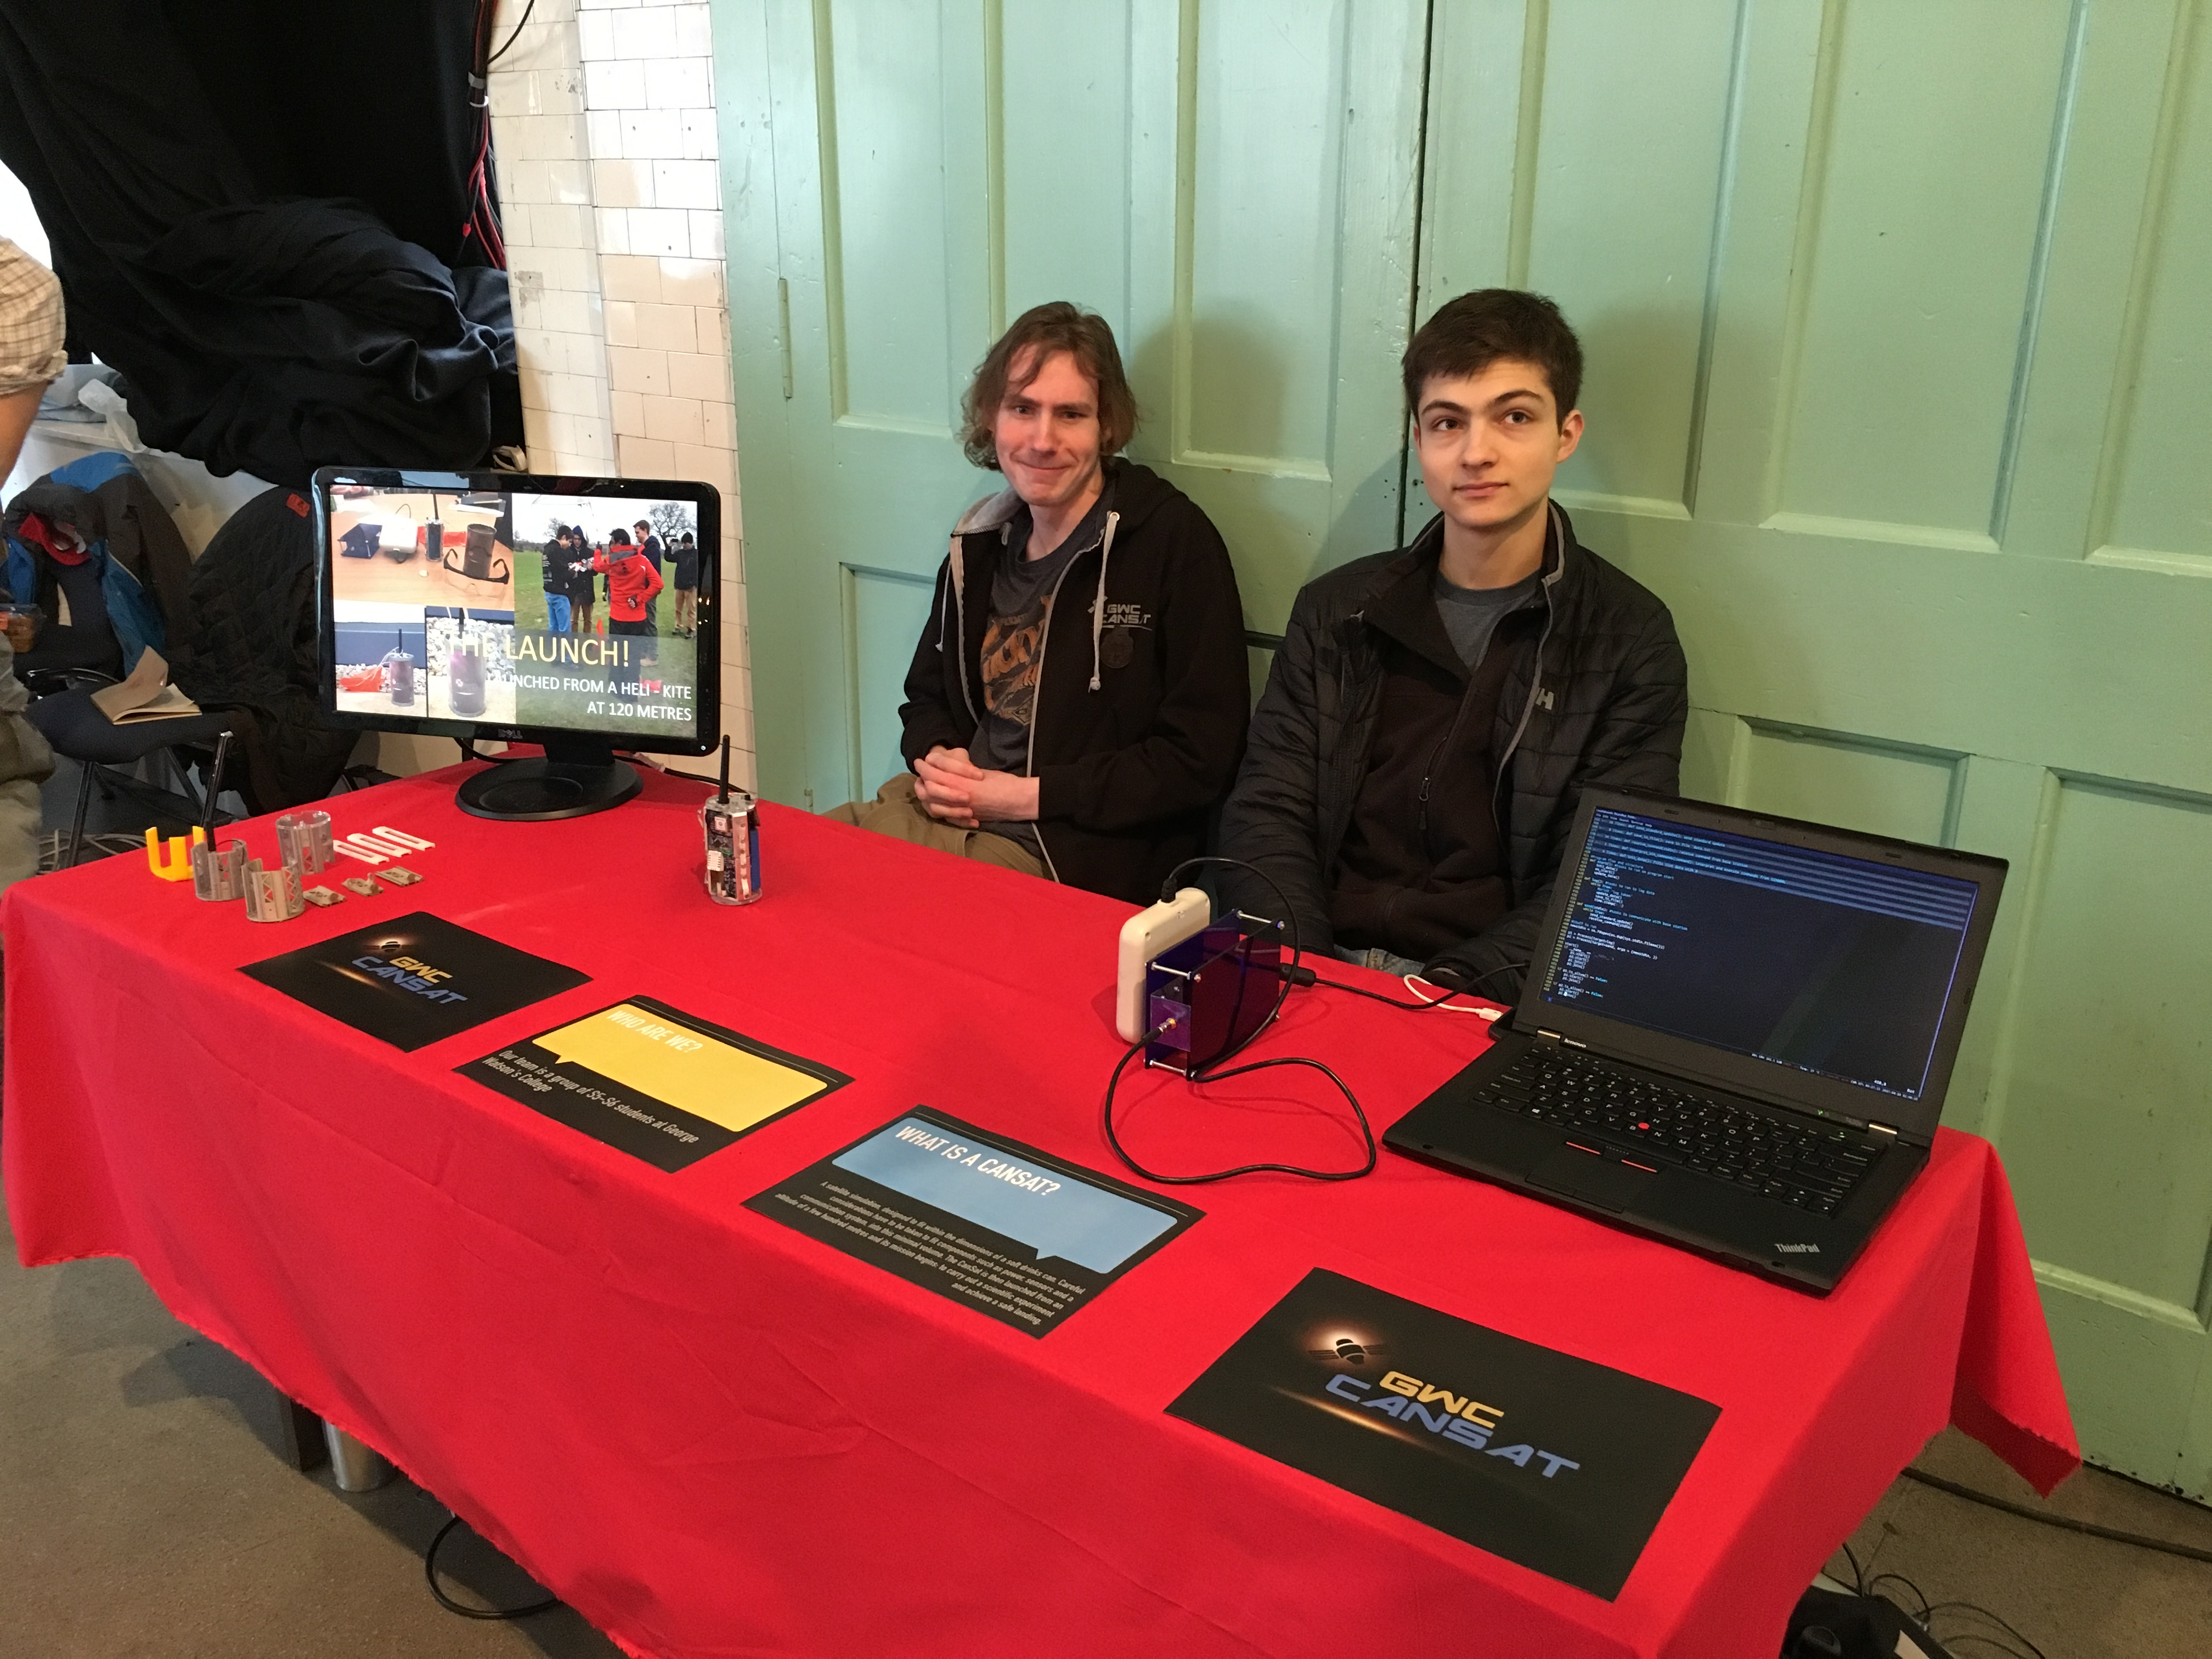
\includegraphics[scale=0.1]{mfaire.jpg}\hspace*{\fill}
	\caption{The team at Edinburgh Mini Maker Fair 2017}
	\label{mfair}
\end{figure}


\chapter{CanSat Requirement Specifications}

\begin{center}
\begin{tabular}{ll}
	Specification          & Value      \\ \hline
	CanSat Height           & 115mm      \\
	CanSat Mass             & 303g       \\
	CanSat Diameter         & 65mm       \\
	Recovery System Length  & 30mm       \\
	Scheduled Flight Time   & 95s        \\
	Calculated Descent Rate & 10.5ms-1   \\
	Radio Frequency Used    & 863-870MHz \\
	Power Consumption       & 403mA      \\
	Total Cost              & 313 EUR    \\
\end{tabular}
\end{center}

\end{document}          
